% Setting up the IEEE journal template with necessary packages
\documentclass[conference,twoside]{IEEEtran}
\IEEEoverridecommandlockouts
\usepackage{amsmath, amssymb, amsthm}
\usepackage{graphicx}
\usepackage{algorithm}
\usepackage{algpseudocode}
\usepackage{booktabs}
%\usepackage{cite}
\usepackage[square]{natbib}
\usepackage{xcolor}
\usepackage{soul}
\usepackage{hyperref}
\hypersetup{
colorlinks = true,
linkcolor = blue,
citecolor = blue,
urlcolor = blue,
filecolor = black,
linktoc = all,
}
\usepackage{times}
\usepackage{geometry}
\geometry{margin=1in}
\usepackage{siunitx}
\usepackage{fancyhdr}
\usepackage{longtable}
\usepackage{parskip}
\usepackage{pgfplots}
\usepackage{natbib}
\usepackage{cite}
\pgfplotsset{compat=1.18}
% Double-column longtable
\sisetup{round-mode=places, round-precision=0}
\setlength{\parskip}{1em}
\pagestyle{fancy}
\fancyhf{} % Clear default headers/footers
\fancyfoot[RO]{\thepage} % Bottom right for odd pages
\fancyfoot[LE]{\thepage} % Bottom left for even pages
\setlength{\parskip}{0pt}
\setlength{\parindent}{0pt}
\usepackage{subcaption}

% Ensuring proper document structure
\begin{document}

% Defining the title
\title{Insights and Limitations of Shor's Factorization Algorithm on IBM Real Quantum Computers}

% Author information
\author{\IEEEauthorblockN{Authors: Juan Manuel Villarreal D'Angelo, Gerard De Manresa, and Adriano Camps\\
Tutor: Joseph Schindler}
\IEEEauthorblockA{\textit{Quantum Engineering Post-graduate Course (2024-2025) - Final project} }
\textit{Fundació Politècnica de Catalunya, Barcelona, Spain }\\
juanmav07@gmail.com, gdemanjo@gmail.com, adriano.jose.camps@upc.edu\\jcschindler01@gmail.com}

% Generating the title
\maketitle

% Abstract section (~250 words)
\begin{abstract}
Quantum Shor's algorithm offers an exponential speedup over classical methods for integer factorization, a central problem to modern cryptography, and the implications of Shor's algorithm in factoring large numbers. The algorithm leverages on quantum parallelism to compute the period of a modular exponentiation function, employing the Inverse Quantum Fourier Transform (IQFT) to extract periodicity, and classical post-processing to derive the factors. This final report of the Quantum Engineering post-graduate course of the Fundació Politènica de Catalunya, presents the main findings encountered in the implementation and benchmarking of Schor's algorithm in real IBM quantum computers. To accomplish this, we created a command line tool made in Python, that allows the integration of the circuits implementing the Shor's algorithm with the overall set of configuration parameters needed to perform the benchmark. In this report, we first provide an overview of the quantum factoring problem, followed by a detailed description of Shor’s algorithm, and its implementation using the Qiskit Python library. The circuit depth and noise effects are analyzed across different backend types, also different values for the optimization level and approximation degrees are configured when performing the circuit transpilation. As mentioned earlier different backend types were utilized for performance comparison, namely backend class with or without a noise model (AerSim), a fake backend class provided by the Qiskit library (fake provider), and the real quantum hardware (IBM Quantum Processing Units in January-June 2025).\iffalse The circuit depth and noise effects are analyzed in real hardware by computing gate counts and circuit depths for factoring $N = 15$ across different values of $a$ using the AerSim backend and two quantum computers: \texttt{ibm\_brisbane} (Eagle r3, 127 qubits) and \texttt{ibm\_torino} (Heron r1, 133 qubits) with distinct architectures. We test different optimization levels (0-3) and approximation degrees (0.5, 0.7, 1.0) when transpiling the quantum circuits. For the optimal $a$ value, circuit depths are compared across ideal simulation, AerSim backend, Fake Provider, and actual quantum hardware including \texttt{ibm\_brisbane}, \texttt{ibm\_torino}, and \texttt{ibm\_aachen} (155 qubits, the most powerful system available as of March-June 2025)\fi The study follows by analyzing the different error mitigation techniques: dynamic decoupling, Pauli twirling, the SABRE Optimization (Stochastic Algorithm for Quantum Boolean Optimization and Routing), and any combination of them. Once the optimum configuration is found, the maximum number that can be reasonably factorized with success is explored. Finally, the main conclusions, findings, and possible future research lines are presented, including the factorization of a $N \approx 1000$ if appropriate parameters of the algorithm are selected.
\end{abstract}


% IEEE keywords
\begin{IEEEkeywords}
Quantum Computing, Shor's Algorithm, Factorization, Quantum Fourier Transform, Modular Exponentiation, Cryptography
\end{IEEEkeywords}

% Introduction section
\section{Introduction}
% Providing an overview of the quantum factoring problem
Integer factorization is a computationally hard problem underpinning the security of widely used cryptographic systems like RSA. Classical algorithms, such as the quadratic sieve or general number field sieve, factor large integers in sub-exponential time, making them inefficient for large numbers. Shor's algorithm, introduced by Peter Shor in 1994 \citep*{shor1994}, leverages on quantum computing to achieve polynomial-time factorization, posing a potential threat to RSA-based encryption. The first experimental demonstration of Shor's algorithm dates from 2001\citep*{Vandersypen2001}, when $N=15$ was factored. In 2007 Lu et al.\citep*{Lu2007} factorized $N=15$ using a photonic implementation.  As of today, the largest numbers factorized by true Shor's algorithm is $N=21$ on actual quantum hardware (2012)\citep*{Martin-Lopez2012}, and in an IBM quantum processor in 2021 \citep*{Karamlou2021}. In \citep*{Gidney2021} it is estimated that factoring a security-standard 2,048-bit number would require a quantum computer with 20 million qubits.
\\
This work explores Shor's algorithm, detailing its components—modular exponentiation, Quantum Fourier Transform (QFT), and classical post-processing—and their roles in achieving quantum speedup. We also address practical challenges, including circuit depth and noise in quantum hardware, which limit current implementations. Additionally, a Python-based simulation using Qiskit\citep*{qiskit2023} is described to illustrate the algorithm's mechanics for small integers. The significance of circuit depth and noise is analyzed to highlight barriers to scaling Shor's algorithm on real quantum devices, emphasizing the need for advancements in quantum error correction.

% Detailed description of Shor's algorithm
% Modular exponentiation
\section{Shor's Algorithm}

Before entering in depth in the description of the algorithm itself, its implementation, and the results obtained, we will explain Shor's algorithm in a simple way. Shor's algorithm is a way to break down large numbers into their smaller building blocks (called prime factors), for example, breaking 15 into 3 × 5. This is important because most of our internet security relies on the fact that factoring huge numbers (with hundreds of digits) is nearly impossible for regular computers, so if you can factor these numbers quickly, you can break encryption. 

\subsection{Shor's Algorithm for Dummies}
Shor's algorithm relies on finding a hidden pattern. Let's try to illustrate it with an example, trying to factorize the number 15.
\begin{itemize}
    \item \textbf{Initialization}: pick a random number smaller than 15 that doesn't share factors with 15, for example 7.
    \item \textbf{Finding the repetition pattern}: \iffalse This is the $magic$ quantum part.\fi we look at powers of 7, but we will only care about the remainder after dividing it by 15. For example, \(7^{0} = 1\) (the remainder of 1 when divided by 15 is 1), \(7^{1} = 7\) (remainder 7), \(7^{2} = 49\) (remainder 4), \(7^{3} = 343\) (remainder 13), \(7^{4} = 2401\) (remainder 1), so we are back to 1. It is clear now that the pattern repeats every 4 steps: 
    1 → 7 → 4 → 13 → 1 → 7...
    \item \textbf{Factorization}: Here, we use the pattern to find the factors. Since the pattern length is 4, we calculate: \(7^{4/2} = 7² = 49 \), then we compute \(49 - 1 = 48\) and \(49 + 1 = 50\).
    \item \textbf{Finding the greatest common divisor}: The final step is to find the greatest common divisor (gcd) of the previous two numbers: 
    \begin{equation}
     gcd(48, 15) = 3, % gcd(48, 15) = 3 \  ✓,
     gcd(50, 15) = 5, % gcd(50, 15) = 5 \  ✓,
    \end{equation}
Finally, the result is 15 = 3 × 5.
\end{itemize}

The quantum part relies on superposition to find the pattern length much faster than a classical computer by testing many possibilities simultaneously, as opposed to test each power one by one, which is much slower. Real encryption uses numbers with hundreds of digits. Finding their repeating patterns would take classical computers forever, but quantum computers could potentially do it in reasonable time. However, today's quantum computers can only handle simple examples like this one, and we would need thousands of error-corrected qubits to threaten real encryption that uses 300+ digit numbers.

Figure~\ref{fig:Schor_circuit} illustrates the implementation of Shor's factorization algorithm for $N=15$ and $a=4$. \iffalse For other values of $a$, but same value of $N$, only the first module \texttt{4 mod 15} has to be changed.\fi Here is a description of the circuit architecture: 

\begin{itemize}
\item \textbf{Initialization of the qubits and application of Hadamard gates (left section):} Control Register are 9 qubits labeled \texttt{control0} to \texttt{control8}, that are used to create a superposition of states and store the input \( x \) for the function \( f(x) \). Note that the number of control qubits should be larger than \(n_1 = 2\lceil \log_2 15 \rceil +1 =  9 \). Target Register are 4 qubits labeled \texttt{target0} to \texttt{target3}. We need enough qubits to represent numbers up to 15. With 4 qubits, we can represent values from 0 to 15 (since \( 2^4 = 16 \)), which is sufficient. These hold the output of the function \( f(x) = a^x \mod {15} \). Finally, output (lower line) is not a qubit, but represents the final measurement of the control register after the Inverse Quantum Fourier Transform (IQFT), which gives the period.
\item \textbf{Modular exponentiation (middle section):} computes \( f(x) = a^x \mod {15} \) for each \( x \) (Figure~\ref{fig:fig1}), and the result is stored in the control qubits.
\item \textbf{Inverse Quantum Fourier Transform - IQFT (right Section):} The IQFT converts the superposition of \( x \) values into a superposition of frequencies. Peaks in the frequency domain correspond to the period \( r \), as illustrated in figure ~\ref{fig:three_figures} obtained in a real QPU for different values of $a$. Clean peaks at 0 and 0.5, i.e. separation equal to 1/2, corresponds to $r=2$, and peaks at 0 and 0.25, 0.5, 0.75, i.e. separation equal to 1/4, correspond to $r=4$.
\item \textbf{Measurement (rightmost section):} After the IQFT, measuring the control qubits (gray gauges) gives a value related to \( {2^9} / {r} \), which can be used to determine \( r \) in a classical way. 
\end{itemize}

This circuit demonstrates the core quantum part of Shor's algorithm: the use of superposition and the IQFT to find the period of a function efficiently.

\begin{figure}[t]
    \centering  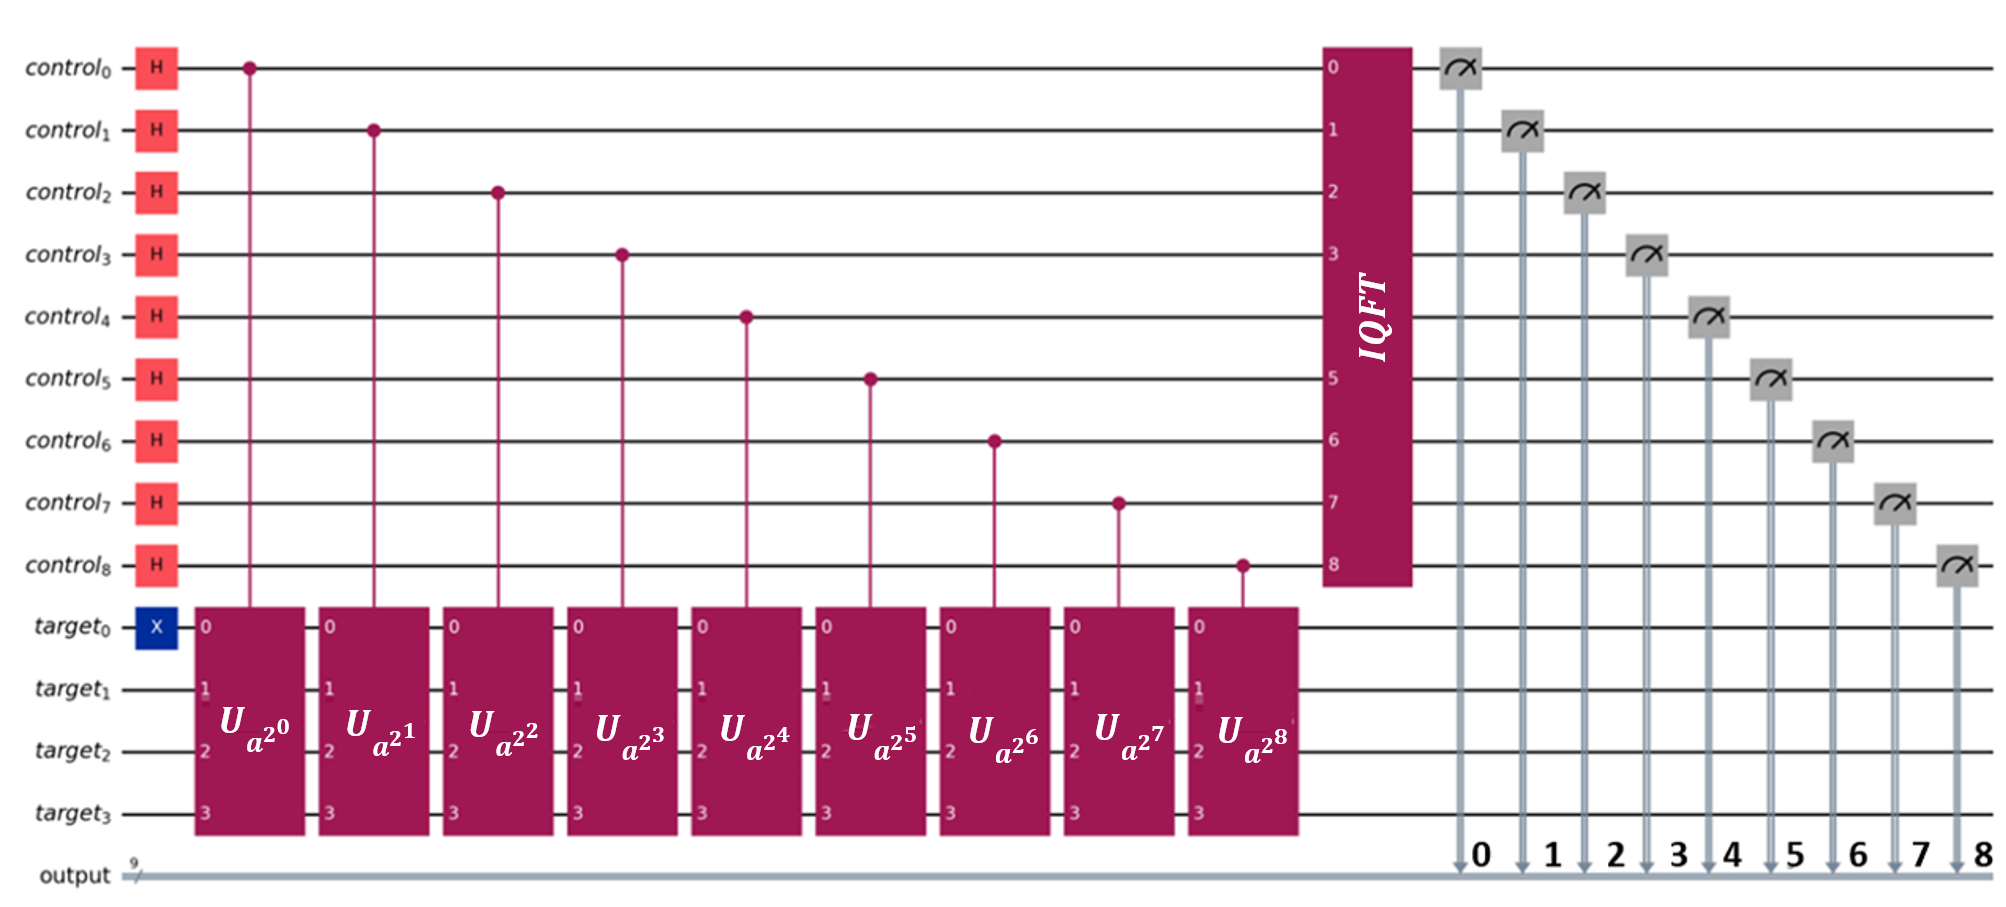
\includegraphics[width=1\columnwidth,keepaspectratio]{New_Fig1.png}
    \caption{Quantum circuit implementing Shor's algorithm for $N=15$ and $a=4$.}
    \label{fig:Schor_circuit}
\end{figure}

\begin{figure}[t]
    \centering  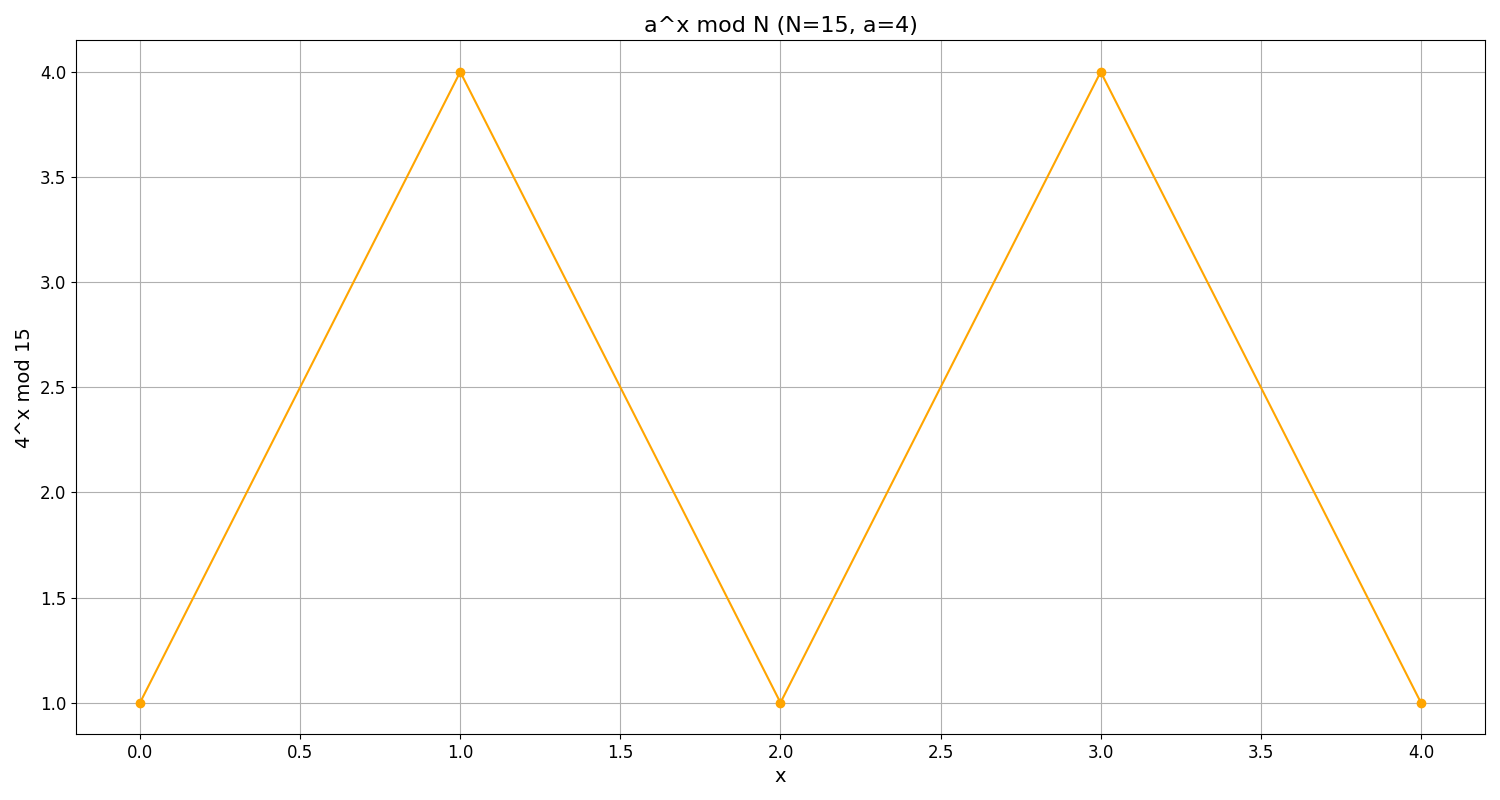
\includegraphics[width=0.9\columnwidth,keepaspectratio]{ax_mod_N15_a4.png}
    \caption{Sample periodic function \(a^x \mod N\), $a=4$, $N=15$ whose period we try to find.}
    \label{fig:fig1}
\end{figure}

% Figure environment spanning both columns
\begin{figure*}[!htbp]
    \centering
    \begin{minipage}{0.3\textwidth}
        \centering
        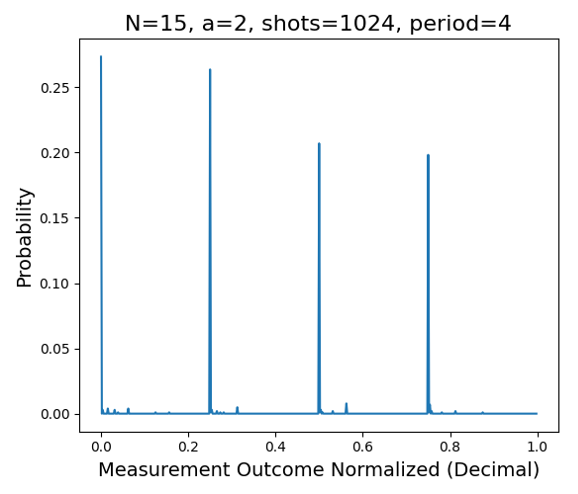
\includegraphics[width=\linewidth]{prob_dist_N15_a2_backend_aersim.png}
        \label{fig:first}
        \small (a)
    \end{minipage}\hspace{0.03\textwidth}
    \begin{minipage}{0.3\textwidth}
        \centering
        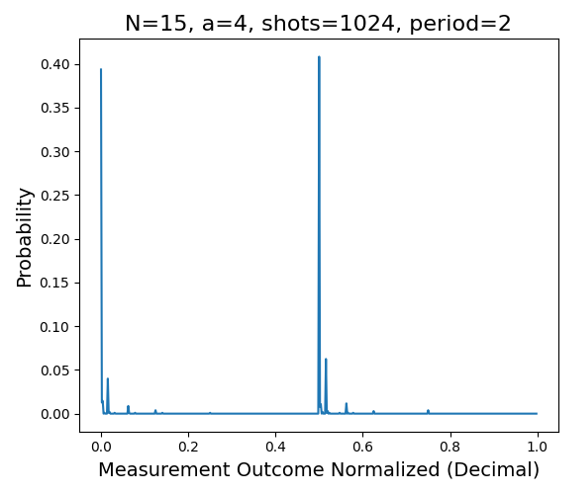
\includegraphics[width=\linewidth]{prob_dist_N15_a4_backend_aersim.png}
        \label{fig:second}
        \small (b)
    \end{minipage}\hspace{0.03\textwidth}
    \begin{minipage}{0.3\textwidth}
        \centering
        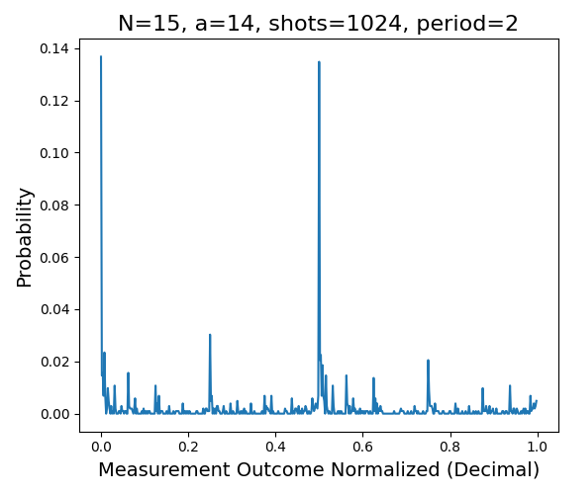
\includegraphics[width=\linewidth]{prob_dist_N15_a14_backend_aersim.png}
        \label{fig:third}
        \small (c)
    \end{minipage}
    \caption{Estimated phases from the order finding circuit for different values of $a$ in a real QPU (same parameters in all three cases, irrelevant at this stage to understand the operation of the algorithm): a) Peak separation is 1/4. $r = 4$, b-c) Peak separation is 1/2. $r = 2$}
    \label{fig:three_figures}
\end{figure*}

\subsection{Shor's Algorithm: Detailed Explanation}
In this Section we will explain in detail the different operations that take place in the computation of the Shor's algorithm.

\subsubsection{Modular Exponentiation}
% Introducing the role of modular exponentiation
Modular exponentiation is the computational core of Shor's algorithm, enabling the quantum speedup that makes integer factorization exponentially faster than classical methods\footnote{For a comprehensive introduction to Shor’s algorithm and its quantum foundations, see \citep*{nielsen2010}.}. Given an integer \( N \) to be factored and a randomly chosen integer \( a \) such that \( \gcd(a, N) = 1 \), Shor's algorithm aims to find the order \( r \), the smallest positive integer satisfying \( a^r \equiv 1 \mod N \). The function \( f(x) = a^x \mod N \) is periodic with order \( r \), and computing this function quantumly exploits superposition to evaluate it for many values of \( x \) simultaneously, a key feature distinguishing quantum from classical approaches. 

% Quantum state preparation
The quantum circuit for modular exponentiation operates on two registers. The first register, with \( n_1 = 2 \lceil \log_2 N \rceil + 1 \) qubits\footnote{\(  \lceil \ \rceil\) denotes the "ceil" function: round to the immediately larger integer.}, encodes the input \( x \). The second register, with \( n_2 = \lceil \log_2 N \rceil \) qubits, stores the output \( f(x) \). The algorithm begins by initializing the first register in a uniform superposition using Hadamard gates applied to each qubit:
\begin{equation}
|\psi_0\rangle = \frac{1}{\sqrt{2^{n_1}}} \sum_{x=0}^{2^{n_1}-1} |x\rangle |+\rangle.
\end{equation}
The modular exponentiation is implemented via a unitary operator \( U_f \), defined as:
\begin{equation}
U_f |x\rangle |y\rangle = |x\rangle |y \cdot a^x \mod N\rangle,
\end{equation}
where \( y \) is initially \( |1\rangle \) in the second register to handle multiplicative operations. Applying \( U_f \) to the initial state produces:
\begin{equation}
|\psi_1\rangle = \frac{1}{\sqrt{2^{n_1}}} \sum_{x=0}^{2^{n_1}-1} |x\rangle |a^x \mod N\rangle.
\end{equation}

This entangled state encodes the periodic function \( f(x) \), with the order \( r \) embedded in the first register's values (\texttt{control0} to \texttt{control8}), setting the stage for the subsequent period finding via the Quantum Fourier Transform. 
% Classical analogy and quantum adaptation
Classically, modular exponentiation is computed efficiently using the square-and-multiply algorithm, which reduces the number of multiplications to \( O(\log_2 x) \). Quantum implementations of such arithmetic operations are discussed in \citep*{vedral1996}. For an exponent \( x \) represented in binary as \( x = \sum_{j=0}^{n_1-1} x_j 2^j \), the exponentiation is:
\begin{equation}
a^x \mod N = \prod_{j=0}^{n_1-1} (a^{2^j} \mod N)^{x_j}.
\end{equation}
In the quantum circuit, this is implemented as a sequence of \( n_1 \) controlled modular multiplications. For each qubit \( |x_j\rangle \) in the first register, a controlled operation multiplies the second register by \( a^{2^j} \mod N \),  if \( x_j = 1 \). The values \( a^{2^j} \mod N \) can be precomputed classically to reduce quantum gate count, though on-the-fly computation is possible for generality.

% Quantum circuit construction
Each modular multiplication is a reversible quantum operation. To multiply the second register by \( b = a^{2^j} \mod N \), a quantum circuit performs:
\begin{equation}
|y\rangle \to |y \cdot b \mod N\rangle,
\end{equation}
conditioned on \( |x_j\rangle = |1\rangle \).
Appendix 1 presents the implementation of the the exponential multiplication, and discusses ways to optimize it.
\\
\subsubsection{Inverse Quantum Fourier Transform}
% Overview and role in Shor's algorithm
The Inverse Quantum Fourier Transform (IQFT) is a critical component of Shor's algorithm, enabling the extraction of the order \( r \) of the function \( f(x) = a^x \mod N \), where \( N \) is the integer to be factored and \( a \) is a randomly chosen integer such that \( \gcd(a, N) = 1 \). The direct QFT transforms a quantum state encoding the input register into the frequency domain, amplifying states corresponding to multiples of the period's reciprocal, thus facilitating period finding. This is a fundamental step to achieve the exponential speedup of Shor's algorithm over classical factorization methods, as it efficiently identifies the periodicity that leads to \( N \)'s factors.

% Mathematical foundation
The QFT is the quantum analog of the classical discrete Fourier transform, operating on an \( n \)-qubit register with basis states \( |0\rangle, \ldots, |2^n-1\rangle \). For an input state \( |x\rangle \), where \( x = \sum_{j=0}^{n-1} x_j 2^j \) is the binary representation, the QFT is defined as:
\begin{equation}
\text{QFT} |x\rangle = \frac{1}{\sqrt{2^n}} \sum_{k=0}^{2^n-1} e^{2\pi i x k / 2^n} |k\rangle.
\end{equation}
In Shor's algorithm, the IQFT is applied to the first register (with \( n_1 =  \lceil 2 \log_2 N \rceil +1 \) qubits) after modular exponentiation, which produces the state given in eqn. (4).
Since \( f(x) = a^x \mod N \) is periodic with order \( r \), the first register’s state can be approximated (ignoring phase offsets for simplicity) as a superposition of states \( |x\rangle \) where \( f(x) \) repeats. Because of the periodicity of \( f(x) \), the application of the IQFT to \(|\psi_1\rangle \) makes the amplitudes to have peaks at values of \( k \approx 2^{n_1} j / r \), where \( j \) is an integer. Measuring the first register yields \( k \), which is used to estimate \( r \) via classical post-processing (e.g., continued fraction algorithm). Appendix 2 presents the QFT implementation and some ways to optimize it.
\\
\subsubsection{Classical Post-Processing}
% Overview and role in Shor's algorithm
Classical post-processing is the final step in Shor's algorithm, transforming the quantum measurement output into the factors of the composite integer \( N \). After modular exponentiation and the Inverse Quantum Fourier Transform (IQFT), the algorithm measures the first register to obtain a value \( k \), which encodes information about the order \( r \) of the function \( f(x) = a^x \mod N \), where \( a \) is a randomly chosen integer satisfying \( \gcd(a, N) = 1 \) \footnote{The selection of \(a\) plays a critical role in the success of Schor's algorithm, as \(a\) has to be a coprime number of \(N\). If if is not, the transpilation of the code gives an error, as the matrices \(U_b\) are not unitary. For small values of \(N\), as the values that can be factored in today's QPU's, we can know a priori the list of coprime factors smaller than \(N\), but for very large numbers, as the ones used in cryptography, the values of \(a\) are selected randomly.}. The classical post-processing step uses the continued fraction algorithm to extract \( r \), then computes the greatest common divisor (gcd) to derive non-trivial factors of \( N \). This step is critical, as it connects the quantum computation’s probabilistic output with deterministic factor extraction, completing the factorization process with high probability.
Measuring the first register yields \( k \), an integer between 0 and \( 2^{n_1} - 1 \). The goal is to estimate \( r \) from the fraction \( k / 2^{n_1} \), which approximates \( j / r \) for some \( j \) coprime to \( r \). The continued fraction algorithm is used to find the convergent \( j/r \) such that:
\begin{equation}
\left| \frac{k}{2^{n_1}} - \frac{j}{r} \right| \leq \frac{1}{2^{n_1+1}}.
\end{equation}
This ensures \( r \) is accurately recovered with high probability, provided \( n_1 \) is sufficiently large. The continued fraction algorithm expansion of a real number \( \alpha = k / 2^{n_1} \) is computed as:
\begin{equation}
\alpha = a_0 + \frac{1}{a_1 + \frac{1}{a_2 + \frac{1}{\ddots}}},
\end{equation}
where \( a_i \) are integers obtained via:
\begin{itemize}
    \item Set \( \alpha_0 = \alpha \).
    \item For each \( i \), compute \( a_i = \lfloor \alpha_i \rfloor \), \( \alpha_{i+1} = 1 / (\alpha_i - a_i) \), until \( \alpha_i \) is integer or the expansion terminates.
\end{itemize}
The convergents of the continued fraction are fractions \( p_m / q_m \), computed recursively:
\begin{itemize}
    \item Initialize: \( p_0 = a_0 \), \( q_0 = 1 \); \( p_1 = a_0 a_1 + 1 \), \( q_1 = a_1 \).
    \item For \( m \geq 2 \): \( p_m = a_m p_{m-1} + p_{m-2} \), \( q_m = a_m q_{m-1} + q_{m-2} \).
\end{itemize}
The convergent \( p_m / q_m \) with \( q_m \leq N \) and \( \gcd(p_m, q_m) = 1 \) is a candidate for \( j/r \). The denominator \( q_m \) is tested as the period \( r \).

% Factor extraction
Once \( r \) is found, it is checked for suitability:
\begin{itemize}
    \item \( r \) must be even (since odd periods do not yield factors in this context).
    \item \( r \) validates the equation: \( a^{r} \equiv 1 \mod N \).
    \item \( a^{r/2} \not\equiv 1 \mod N \), to avoid trivial results.
\end{itemize}
If these conditions hold, the factors of \( N \) are computed as:
\begin{equation}
f_1 = \gcd(a^{r/2} - 1, N), \quad f_2 = \gcd(a^{r/2} + 1, N).
\end{equation}
The gcd is efficiently computed using Euclid’s algorithm, which has complexity \( O((\log_2 N)^2) \) \footnote{The Euclidean Algorithm is a method to find the greatest common divisor (gcd) of two non-negative integers. It is based on the principle that the gdc of two numbers also divides their difference. The procedure is as follows: given two non-negative integers \(a\) and \(b\), where \(a \geq b\), divide \(a\) by \(b\) to obtain a quotient \(q\) and remainder \(r\), such that \( a = b \cdot q + r, \quad 0 \leq r < b\). If \(r = 0\), then \(b\) is the gcd, but if \(r \neq 0\), then set \(a = b\), \(b = r\), and repeat the previous step, The gcd is the last non-zero remainder.}  If \( f_1 \) or \( f_2 \) are non-trivial (i.e., \( 1 < f_i < N \)), they are factors of \( N \). If \( r \) is invalid or yields trivial factors, the algorithm repeats with a new \( a \).

% Success probability
The success of classical post-processing depends on the IQFT outputting \( k \) such that \( k / 2^{n_1} \approx j / r \) with \( \gcd(j, r) = 1 \). Shor's analysis shows this occurs with probability at least \( \phi(r) / r \geq 1 / (2 \log_2 \log_2 r) \), where \( \phi \) is Euler’s Totient function \footnote{Euler's Totient Function, denoted \(\phi(n)\), counts the number of positive integers up to a positive integer \(N\) that are coprime to \(N\). Two integers are coprime if their greatest common divisor (gcd) is 1. Thus, \(\phi(N)\) is the number of integers \(k\) in the range \(1 \leq k \leq N\) such that \(\gcd(k, N) = 1\). For a positive integer \(N\), the totient function is defined as \(\phi(N) = |\{ k \in \mathbb{Z} \mid 1 \leq k \leq N, \gcd(k, N) = 1 \}|
\). If \(N\) has the prime factorization \(N = p_1^{e_1} p_2^{e_2} \cdots p_k^{e_k}\), where \(p_i\) are distinct primes and \(e_i\) are their exponents, then \(
\phi(N) = N \prod_{p \mid N} \left(1 - \frac{1}{p}\right),
\), where the product is over all distinct primes \(p\) dividing \(N\). Cases of interest: for a prime \(p\), \(\phi(p) = p - 1 \), for a prime power \(p^k\), \(\phi(p^k) = p^k - p^{k-1} = p^{k-1}(p - 1) \), and for coprime integers \(m\) and \(n\), \( \phi(m \cdot n) = \phi(m) \cdot \phi(n) \).}  For large \( r \), this probability is sufficiently high, and multiple measurements increase the likelihood of success. The choice of \( n_1 = \lceil 2 \log_2 N \rceil+ 1 \) ensures the continued fraction algorithm converges to the correct \( r \) with high probability.

% Practical considerations
Classical post-processing is computationally efficient, with the continued fraction algorithm and gcd computation both running in polynomial time (\( O((\log_2 N)^3) \)). Unlike quantum steps, this phase is robust, as it relies on well-established classical algorithms. However, the quality of the quantum output \( k \) is critical. Noise in the quantum circuit (e.g., gate errors of \( 10^{-3} \) to \( 10^{-2} \) in 2025 hardware) can distort \( k \), leading to incorrect convergents. Fault-tolerant quantum computing is thus essential for large \( N \). For small \( N \) (e.g., \( N = 15 \)), simulations in Qiskit demonstrate successful period finding (e.g., \( r = 4 \) for \( a = 7 \)), but scaling to cryptographic sizes (e.g., 2048-bit \( N \)) requires error-corrected qubits.

% Pseudocode
The \textbf{algorithm}~\ref{alg:shor_factorization} outlines the Shor's algorithm implementation, and \textbf{algorithm}~\ref{alg:classical_pos} the classical post-processing.

\begin{algorithm}
\caption{Shor's Algorithm Implementation}
\label{alg:shor_factorization}
\begin{algorithmic}
\State \textbf{Input}: Number \( N \), arguments (\texttt{args}), \( a \)-coefficients
\State \textbf{Output}: Factors of \( N \)
\State Check if \( N \) is even or a prime power; return factors if true
\State Compute \( \gcd(a, N) \); return factors if \( \gcd \neq 1 \)
\State Initialize \texttt{Shor} with backend, sampler, transpiler parameters
\For{each \( a \) in \( a \)-coefficients}
    \State Create circuit:
    \State \hspace*{1em} Create control (\( n_1 \)), target (\( n_2 = \)) registers
    \State \hspace*{1em} Apply Hadamard gates to control register
    \State \hspace*{1em} Apply controlled modular exponentiation for \hspace*{2.5em} \( a^{2^j} \mod N \)
    \State \hspace*{1em} Apply inverse QFT to control register
    \State \hspace*{1em} Measure control register to obtain \( k \)
    \State Transpile circuit (inlcuding SABRE optimization \hspace*{1em} only if set)
    \State Run sampler with shots (dynamical decoupling \hspace*{1em} and Pauli twirling are included on the sampling \hspace*{1em} only if set)
    \State Process results: compute \( r \) via continued fractions
    \State Compute factors: \( \gcd(a^{r/2} \pm 1, N) \)
    \If{factors are non-trivial}
        \State \textbf{Return}: Factors
    \EndIf
\EndFor
\State \textbf{Return}: Failure (repeat with new \( a \))
\end{algorithmic}
\end{algorithm}

% Pseudocode

\begin{algorithm}
\caption{Classical Post-Processing in Shor's Algorithm}
\label{alg:classical_pos}
\begin{algorithmic}
\State \textbf{Input}: Measured value \( k \), number of qubits \( n_1 \), integer \( N \), base \( a \)
\State \textbf{Output}: Factors of \( N \) or failure
\State Compute \( \alpha = k / 2^{n_1} \)
\State Initialize continued fraction: \( \alpha_0 = \alpha \), \( a_0 = \lfloor \alpha_0 \rfloor \), \( p_0 = a_0 \), \( q_0 = 1 \)
\State Initialize: \( p_1 = a_0 a_1 + 1 \), \( q_1 = a_1 \), where \( a_1 = \lfloor 1 / (\alpha_0 - a_0) \rfloor \)
\For{each \( m = 2, 3, \ldots \) until \( q_m > N \)}
    \State Compute \( \alpha_m = 1 / (\alpha_{m-1} - a_{m-1}) \), \( a_m = \lfloor \alpha_m \rfloor \)
    \State Update: \( p_m = a_m p_{m-1} + p_{m-2} \), \\ \hspace*{4.5em} \( q_m = a_m q_m-1 + q_{m-2} \)
    \If{\( q_m \leq N \) and \( \gcd(p_m, q_m) = 1 \)}
        \State Set \( r = q_m \)
        \If{\( r \) is even and \( a^{r} \equiv 1 \mod N \)}
            \State Compute \( f_1 = \gcd(a^{r/2} - 1, N) \), \\
            \hspace*{8em} \( f_2 = \gcd(a^{r/2} + 1, N) \)
            \If{\( 1 < f_1 < N \) or \( 1 < f_2 < N \)}
                \State \textbf{Return}: \( f_1, f_2 \)
            \EndIf
        \EndIf
    \EndIf
\EndFor
\State \textbf{Return}: Failure (repeat with new \( a \))
\end{algorithmic}
\end{algorithm}

\section{Command-line tool created to benchmark Shor's algorithm quantum circuit}
\label{sec:clt}
% Description
As we introduced in the abstract, in order to accomplish the main objective of performing the benchmark over the Shor's algorithm quantum circuit, we created a command line tool made in Python\citep*{commandLineTool}. Among the main features are:
\begin{itemize}
    \item Account management (IBM cloud authentication).
    \item Parametrization of the quantum circuit instantiated to perform the benchmark, providing the possibility to test different circuits implementations of Shor's algorithm.
    \item Parametrization of the different backend types instantiated, namely, backend class with or without a noise model (AerSim), a fake backend class provided by the Qiskit library (fake provider), and the real quantum hardware (IBM Quantum Processing Units).
    \item Parametrization of the different availables QPUs to utilize when sending the jobs to sample to the IBM cloud. In this project the UPC provided free and payed access to the following IBM QPUs: \texttt{ibm\_aachen}, \texttt{ibm\_strasbourg}, \texttt{ibm\_brussels} for payed access, and \texttt{ibm\_sherbrooke}, \texttt{ibm\_brisbane}, \texttt{ibm\_torino} for free access, all of them under the FPC account on IBM cloud. It should be noted that before this access was provided we had access to \texttt{ibm\_kyiv} with our personal accounts before his decommission on April 18th 2025, this is worth to mention because one of our best results in terms of circuit transpilation and results came up from this QPU.
    \item Parametrization of the main transpilation features when using Qiskit transpiler. 
    \item Parametrization of the SABRE optimization feature when using Qiskit transpiler.
    \item Parametrization of the main sampling features when using Qiskit sampler.
    \item Transpile using a Fake provider (ibm\_kyiv in this case) and then setting the initial layout of the transpiled circuit into another ibm\_qpu transpilation process for circuit depth comparison. The key point is that, the QPU fake provider class and the target QPU need to belong to the same family of processor type.
    \item Save transpiled circuits to disk in order to avoid transpiling them again when sending them to the IBM QPU for sampling.
    \item Obtain results from sampling jobs submitted previously.
    \item Generate all the visual outputs that the current work is presenting: quantum circuit, quantum circuit physical layout, probability distribution for normalized order count, with the circuit statistics and noise percentage included.
    \item Calculate a set of optimal values of $a$ based on the number that we want to factor.
    \item Full integration with Qiskit SDK, Qiskit runtime environment, Qiskit visualization tools.
\end{itemize}


\section{Description of the Implemented Code}
% Overview
The implementation of Shor's algorithm provided leverages Qiskit, a Python-based quantum computing framework, to simulate or execute the algorithm for factoring small (TBD) integers on quantum hardware or simulators. The  code orchestrates the algorithm’s key components: modular exponentiation, Inverse Quantum Fourier Transform (IQFT), and classical post-processing. It supports both classical pre-checks and quantum computation, with optimizations for real quantum hardware, including transpilation and error mitigation. This section details the implementation’s structure, functionality, and practical considerations, highlighting its alignment with Shor's algorithm’s theoretical framework.

% Code structure and entry point
The entry point is \texttt{main.py}, which initializes the program by loading settings and parsing command-line arguments using \texttt{CommandLineParser} and \texttt{ConfigurationIni} classes. It supports two modes: processing results from a previous job (via \texttt{job\_id}) or running Shor's algorithm to factor a number \( N \) (via \texttt{Factorizer}). The \texttt{Factorizer} class in \texttt{arithmetics.py} coordinates the factorization process, performing classical checks (e.g., if \( N \) is even or a prime power) before invoking the quantum algorithm via the \texttt{Shor} class in \texttt{phase\_estimation.py}. The implementation is modular, with separate modules for circuit construction (\texttt{circuit.py}), sampling (\texttt{sampling.py}), and transpilation (\texttt{transpilation.py}).

% Classical pre-processing
In \texttt{arithmetics.py}, the \texttt{Factorizer} class first attempts classical factorization to avoid unnecessary quantum computation. For an input number \( N \), it checks:
\begin{itemize}
    \item If \( N \) is even, it returns factors \( 2 \) and \( N/2 \).
    \item If \( N \) is a prime power (\( N = d^b \)), it identifies factors \( d \) and \( d^{b-1} \).
    \item For a chosen \( a \), it computes \( \gcd(a, N) \). If \( \gcd(a, N) \neq 1 \), it yields the factors directly.
\end{itemize}
If these fail, it selects the coefficients $a$ either randomly, user-specified, or as coprimes of \( N \)), using \texttt{get\_circuits\_coefficients} method, then passes them to the \texttt{Shor} class for quantum period finding.

% Quantum circuit construction
The \texttt{circuit.py} module defines a \texttt{QCircuit} abstract base class and the \texttt{RegisterQC} that inherits from the \texttt{QCircuit} class and implements the \texttt{create\_circuit} method. The \texttt{create\_circuit} method in \texttt{RegisterQC} builds the quantum circuit for a given \( N \) and \( a \):
\begin{itemize}
    \item \textbf{Registers}: Initializes a control register with \( n_1 = 2 \lceil \log_2 N \rceil + 1 \) qubits, a target register with \( n_2 = \lceil \log_2 N \rceil \) qubits, and a classical register for measurements.
    \item \textbf{Initialization}: Applies an X gate to the target register’s least significant qubit (setting it to \( |1\rangle \)) and Hadamard gates to the control register to create a superposition (eqn.(2)).
    \item \textbf{Modular Exponentiation}: For each control qubit \( j \), computes \( b = a^{2^j} \mod N \) classically and applies a controlled unitary gate \( U_f \), where: \(U_f |x\rangle |y\rangle = |x\rangle |y \cdot a^{x} \mod N\rangle.\) (eqn. (3)).
    The unitary is constructed as a permutation matrix in \texttt{b\_mod\_n}, mapping \( |y\rangle \to |b \cdot y \mod N\rangle \), which produces \(|\psi_1\rangle \).
    \item \textbf{IQFT}: Applies an inverse QFT to the control register using Qiskit’s \texttt{QFT} library, transforming the state to amplify amplitudes at \( k \approx 2^{n_1} j / r \).
    \item \textbf{Measurement}: Measures the control register, yielding \( k \).
\end{itemize}

% Transpilation and optimization
The \texttt{transpilation.py} module’s \texttt{Transpiler} class adapts the circuit for specific quantum hardware. It uses Qiskit’s \texttt{pass\_manager} method with parameters like optimization level, basis gates, and routing methods (e.g., SABRE). The \texttt{SabreLayout} class optimizes qubit mapping and routing, with options for multiple iterations and trials to minimize circuit depth and gate count. The \texttt{get\_isa\_statistics} method collects metrics (e.g., two-qubit gate count, circuit depth), critical for assessing hardware feasibility. For example, a circuit for \( N = 15 \) may require hundreds of gates, challenging for NISQ devices with error rates of \( 10^{-3} \) to \( 10^{-2} \).

% Sampling and execution
The \texttt{sampling.py} module defines \texttt{Sampler} classes (\texttt{AerSampler} for simulators, \texttt{IBMRuntimeSampler} for IBM Quantum hardware). The \texttt{Shor} class in \texttt{phase\_estimation.py} orchestrates circuit execution:
\begin{itemize}
    \item Creates circuits for multiple \( a \)-coefficients.
    \item Transpiles circuits using \texttt{Transpiler} class.
    \item Submits jobs to the sampler with configurable shots (e.g., 1024).
    \item Optionally waits for results, processes measurement counts, and extracts candidate orders \( r \) via \texttt{get\_candidate\_rs} method.
\end{itemize}
The \texttt{\_set\_sampler\_params} include error mitigation techniques like dynamical decoupling and Pauli twirling, reducing decoherence and gate errors on real hardware.

% Classical post-processing
Post-processing occurs in \texttt{job\_results.py} via \texttt{find\_nontrivial\_factors} method, which:
\begin{itemize}
    \item Uses the measured \( k \) to compute \( \alpha = k / 2^{n_1} \).
    \item Applies the continued fraction algorithm to find \( r \).
    \item Computes factors as \( \gcd(a^{r/2} \pm 1, N) \).
\end{itemize}
The \texttt{plot\_results\_distribution} function visualizes measurement outcomes, aiding analysis of period candidates.

% Practical considerations
The implementation is optimized for small (TBD) $N$ (e.g., \( N = 15 \)), where \( a = 7 \) yields \( r = 4 \), producing factors 3 and 5. For larger \( N \), the circuit depth (thousands of gates for 2048-bit \( N \)) and noise (gate errors \( \sim 10^{-3} \)) make execution infeasible on current hardware, as it will be shown later. The  code mitigates this with transpilation optimizations and error mitigation, but fault-tolerant quantum computing is required for cryptographic applications.

% Conclusion
This implementation effectively simulates Shor's algorithm for small \( N \), benefiting from Qiskit’s modularity and hardware-aware optimizations. Scaling to cryptographic sizes would require advances in quantum hardware and error correction techniques. In the last section of this report, the authors will explore the maximum achievable $N$ that can be factorized in the available IBM quantum computers.

In order to gain a better understanding on the performance of Shor's algorithm, Figure \ref{fig:fig3} represents the periodicity of the function $a^{x} \ mod \ N$ for $N = 15$, and $a = {2, 3, 4... 14}$. Valid values of $a$ are those that are coprimes\footnote{Coprime numbers are two or more integers that have no common positive divisor other than 1, i.e. their greatest common divisor (gcd) is 1.} of $N$, namely 2, 4, 7, 8, 11, 13 and 14. Values of $a$ that are not coprimes of $N$ will lead to non-unitary matrices and transpilation errors, but in the figure we included them all, as in the original Shor's algorithm the values of $a$ are randomly chosen, and there are high chances that the selected $a$ is not actually a coprime of $N$. 

Additionally, to find the period of the function $a^{x} \ mod \ N$, $a$ must be large enough so that at least two periods of the function fit in $[0, N-1]$, that is: $a_{min}^{N-1} \geq 2N $. For $N \geq 4$, $a_{min} = 2$, so the condition is always satisfied. Table~\ref{tab:min_a} lists all the semiprime numbers smaller than 77, and some of their coprimes. On the other hand, an interesting case occurs when $r = 2$, then for $a = a_{max} = N-1$, then the \( \gcd(a^{r/2} \pm 1, N) = gcd(a \pm 1, N) = gcd(N - 1 \pm 1, N)\) is \(gcd(N - 2, N) = 1\), and \(gcd(N, N) = N\), which are the trivial factors of $N$.


\begin{figure}[t]
    \centering  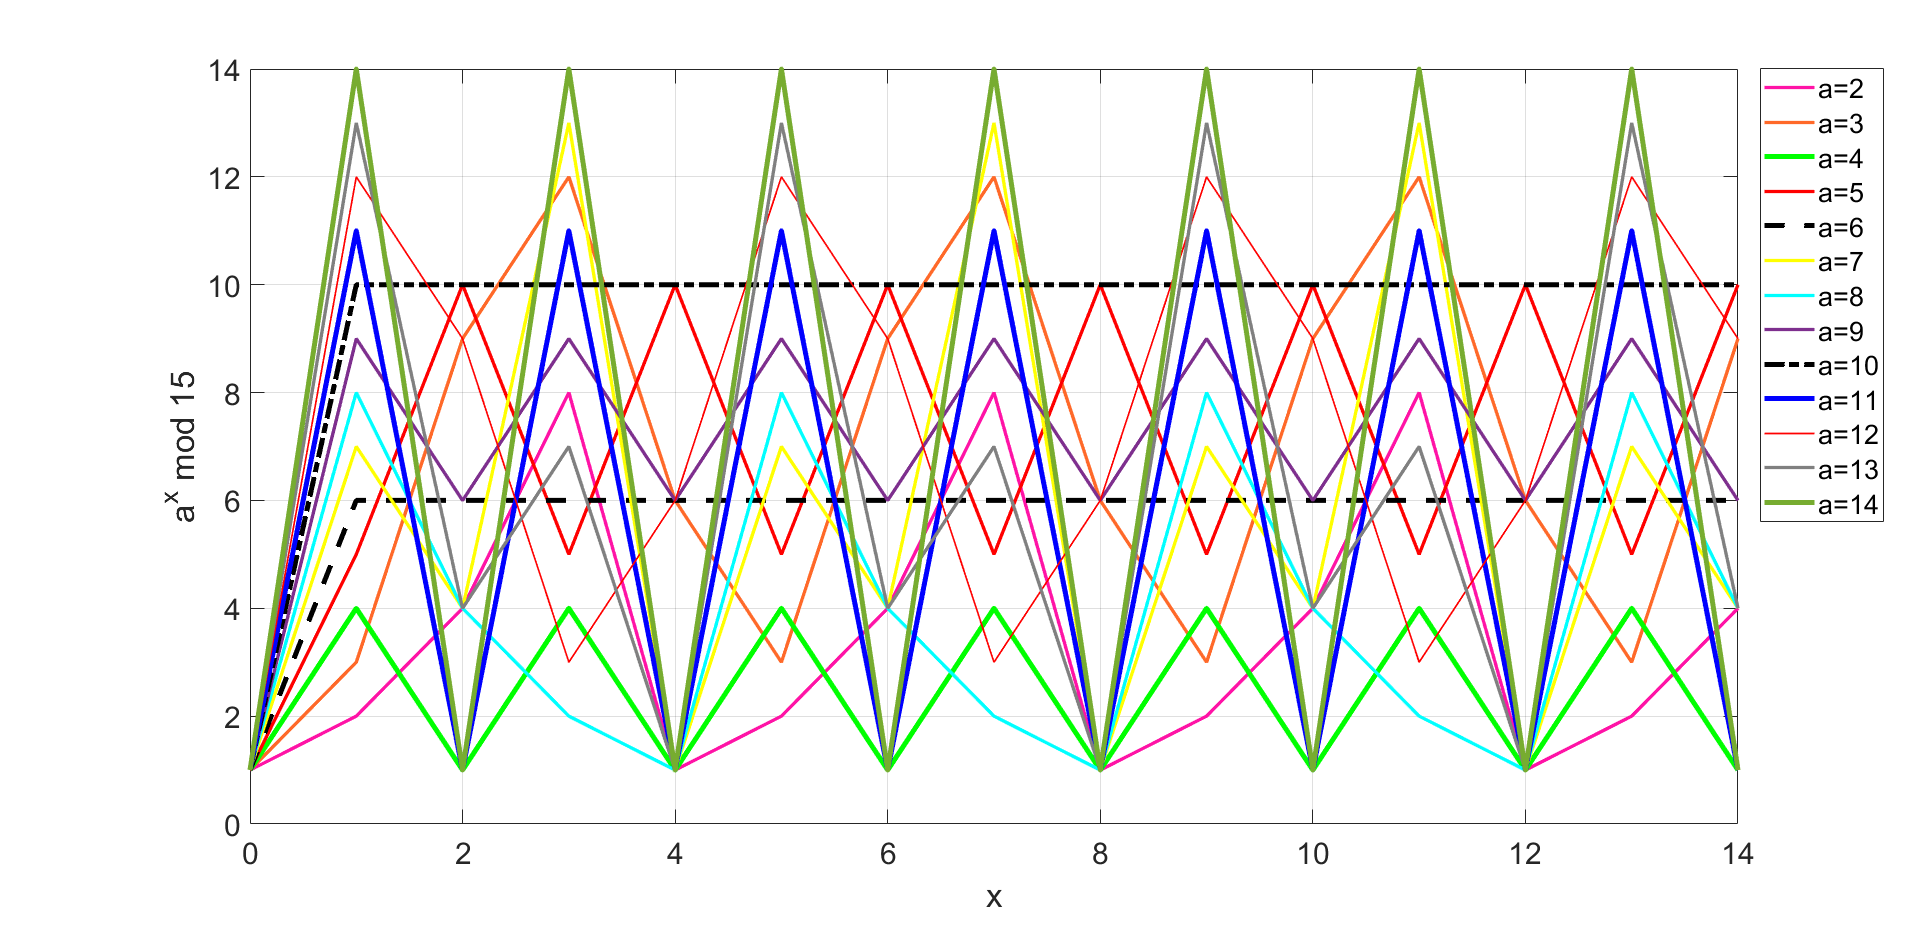
\includegraphics[width=1\columnwidth,keepaspectratio]{Figure_a_x_mod_N.png}
    \caption{Periodicity of $a^{x} \ mod \ N$ for $N = 15$, $a = {2, 3, 4... 14}$. Note that for $a=6, 10$ the plot is flat, and for $a=4$, $a=11$ and $a=14$ there is an integer number of periods.}
    \label{fig:fig3}
\end{figure}


\begin{table}[h]
\centering
\caption{Semiprime numbers smaller or equal than 145, prime factors, coprime numbers smaller than $N$.}
\label{tab:min_a}
\begin{tabular}{c c c c}
\toprule
$N$ & Prime factors & Coprimes $< N$ \\
\midrule
4 & $2 \times 2$ & $1, 3$  \\
6 & $2 \times 3$ & $1, 5$  \\
9 & $3 \times 3$ & $1, 2, 4, 5, 7, 8$  \\
10 & $2 \times 5$ & $1, 3, 7, 9$  \\
14 & $2 \times 7$ & $1, 3, 5, 9, 11, 13$  \\
15 & $3 \times 5$ & $1, 2, 4, 7, 8, 11, 13, 14$  \\
21 & $3 \times 7$ & $1, 2, 4, 5, 8, 10, 11, \ldots, 20$  \\
22 & $2 \times 11$ & $1, 3, 5, 7, 9, 13, 15, \ldots, 21$  \\
25 & $5 \times 5$ & $1, 2, 3, 4, 6, 7, 8, \ldots, 24$  \\
26 & $2 \times 13$ & $1, 3, 5, 7, 9, 11, 15, \ldots, 25$  \\
33 & $3 \times 11$ & $1, 2, 4, 5, 7, 8, 10, \ldots, 32$  \\
34 & $2 \times 17$ & $1, 3, 5, 7, 9, 11, 13, \ldots, 33$  \\
35 & $5 \times 7$ & $1, 2, 3, 4, 6, 8, 9, \ldots, 34$  \\
38 & $2 \times 19$ & $1, 3, 5, 7, 9, 11, 13, \ldots, 37$  \\
39 & $3 \times 13$ & $1, 2, 4, 5, 7, 8, 10, \ldots, 38$  \\
46 & $2 \times 23$ & $1, 3, 5, 7, 9, 11, 13, \ldots, 45$ \\
49 & $7 \times 7$ & $1, 2, 3, 4, 5, 6, 8, \ldots, 48$  \\
51 & $3 \times 17$ & $1, 2, 4, 5, 7, 8, 10, \ldots, 50$  \\
55 & $5 \times 11$ & $1, 2, 3, 4, 6, 7, 8, \ldots, 54$  \\
57 & $3 \times 19$ & $1, 2, 4, 5, 7, 8, 10, \ldots, 56$  \\
58 & $2 \times 29$ & $1, 3, 5, 7, 9, 11, 13, \ldots, 57$  \\
62 & $2 \times 31$ & $1, 3, 5, 7, 9, 11, 13, \ldots, 61$  \\
65 & $5 \times 13$ & $1, 2, 3, 4, 6, 7, 8, \ldots, 64$  \\
69 & $3 \times 23$ & $1, 2, 4, 5, 7, 8, 10, \ldots, 68$ \\
74 & $2 \times 37$ & $1, 3, 5, 7, 9, 11, 13,\ldots, 73$  \\
77 & $7 \times 11$ & $1, 2, 3, 4, 5, 6, 8, \ldots, 76$  \\
82  & \( 2 \times 41 \)  & 1, 3, 5, 7, 9, 11, 13, ... 81 \\
85  & \( 5 \times 17 \)  & 1, 2, 3, 4, 6, 7, 8, ... 84 \\
86  & \( 2 \times 43 \)  & 1, 3, 5, 7, 9, 11, 13, ... 85 \\
87  & \( 3 \times 29 \)  & 1, 2, 4, 5, 7, 8, 10, ... 86 \\
91  & \( 7 \times 13 \)  & 1, 2, 3, 4, 5, 6, 8, ... 90 \\
93  & \( 3 \times 31 \)  & 1, 2, 4, 5, 7, 8, 10, ... 92 \\
94  & \( 2 \times 47 \)  & 1, 3, 5, 7, 9, 11, 13, ... 93 \\
95  & \( 5 \times 19 \)  & 1, 2, 3, 4, 6, 7, 8, ... 94 \\
106 & \( 2 \times 53 \)  & 1, 3, 5, 7, 9, 11, 13, ... 105 \\
111 & \( 3 \times 37 \)  & 1, 2, 4, 5, 7, 8, 10, ... 110 \\
115 & \( 5 \times 23 \)  & 1, 2, 3, 4, 6, 7, 8, ... 114 \\
118 & \( 2 \times 59 \)  & 1, 3, 5, 7, 9, 11, 13, ... 117 \\
119 & \( 7 \times 17 \)  & 1, 2, 3, 4, 5, 6, 8, ... 118 \\
121 & \( 11 \times 11 \) & 1, 2, 3, 4, 5, 6, 7, ... 120 \\
122 & \( 2 \times 61 \)  & 1, 3, 5, 7, 9, 11, 13, ... 121 \\
123 & \( 3 \times 41 \)  & 1, 2, 4, 5, 7, 8, 10, ... 122 \\
129 & \( 3 \times 43 \)  & 1, 2, 4, 5, 7, 8, 10, ... 128 \\
133 & \( 7 \times 19 \)  & 1, 2, 3, 4, 5, 6, 8, ... 132 \\
134 & \( 2 \times 67 \)  & 1, 3, 5, 7, 9, 11, 13, ... 133 \\
141 & \( 3 \times 47 \)  & 1, 2, 4, 5, 7, 8, 10, ... 140 \\
142 & \( 2 \times 71 \)  & 1, 3, 5, 7, 9, 11, 13, ... 141 \\
143 & \( 11 \times 13 \) & 1, 2, 3, 4, 5, 6, 7, ... 142 \\
145 & \( 5 \times 29 \)  & 1, 2, 3, 4, 6, 7, 8, ... 144 \\
\bottomrule
\end{tabular}
\end{table}


% Materials and Methods section
\section{Materials and Methods}
In this Section we first analyze the Circuit Depth and the Total Number of Gates for the thre QPUs available in the free IBM plan, namely \texttt{ibm\_Kyiv}, \texttt{ibm\_Brisbane}, \texttt{ibm\_Sherbrooke}, \texttt{ibm\_Torino} vs. those in the pay per use QPUs, namely \texttt{ibm\_Aachen}, \texttt{ibm\_Brussels}, \texttt{ibm\_Strasbourg}... Then, we revise the quantum hardware specifications, and we finalize with an analysis of the different error mitigation and optimization techniques, namely the Dynamical Decoupling, the Pauli Twirling, and the SABRE Optimization, respectively. To do this, the tool presented in Section \ref{sec:clt} was used.

\subsection{Quantum Hardware}
IBM quantum computing resources available for this work are categorized into free and paid tiers, each offering distinct access levels and capabilities for implementing algorithms like Shor's. Free-tier access, typically provided through platforms like IBM Quantum Experience, allows researchers to experiment with quantum hardware and simulators at no cost, but with significant limitations. These include restricted access to a subset of quantum processors (often smaller systems with fewer qubits, e.g., 127-qubit systems like \texttt{ibm\_kyiv}, \texttt{ibm\_brisbane} and \texttt{ibm\_sherbrooke}), limited monthly runtime (e.g., 10 minutes), and lower priority in job queues, leading to longer wait times. For Shor's algorithm, which requires deep circuits with thousands of gates for factoring even small numbers (e.g., \( N = 15 \)), free-tier access often results in incomplete executions due to time constraints and noise accumulation on NISQ devices.

Paid-tier access, such as IBM Quantum’s Premium or Enterprise plans, unlocks advanced hardware like \texttt{ibm\_aachen}, \texttt{ibm\_brussels}, and \texttt{ibm\_strasbourg}, with higher qubit counts (156 qubits) and improved error rates (e.g., \( 6.28 \times 10^{-4} \) to \( 3.84 \times 10^{-3} \) for two-qubit gates). These plans offer dedicated runtime, and higher queue priority. For Shor's algorithm, paid hardware enables execution of larger circuits with better fidelity, which is crucial for period finding and factorization of numbers beyond toy examples. However, even paid-tier systems struggle with cryptographic-scale \( N \) (e.g., 2048-bit), requiring fault-tolerant quantum computing not yet available in 2025. The choice between free and paid hardware thus balances cost, accessibility, and the feasibility of executing Shor's algorithm effectively.  

In this study we have used only the following IBM Quantum processors to implement Shor's algorithm, specifically \texttt{ibm\_aachen}, \texttt{ibm\_torino}, \texttt{ibm\_brisbane}, and at the beginning of the semester also \texttt{ibm\_Kyiv} which exhibit outstanding performances. Their specifications, including processor type, number of qubits, two-qubit gate error rates (best, layered, and median), coherence times, CNOT-length operations per second and basis gates \footnote{2 qubit gates: ECR gate (Echoed Cross-Resonance Gate): a native entangling gate in IBM's superconducting QPUs, that uses cross-resonance interactions with an echo sequence to reduce noise, modulating the target qubit based on the control qubit's state via microwave pulses. CZ (Controlled-Z Gate): applies a Z (phase flip) operation to the target qubit if the control qubit is in the $\ket{1}$ state, introducing a $\pi$ phase shift to the $\ket{11}$ state, RZZ (Rotation around ZZ Axis): applies a rotation by an angle $\theta$ around the ZZ axis of the two-qubit Pauli operator ($Z \otimes Z$), introducing a phase to the $\ket{11}$ state, used in variational algorithms or error correction, reducing circuit depth. 1 qubit gates: ID (Identity Gate), RX (Rotation around X Axis of the Bloch sphere by an angle $\theta$), RZ (Rotation around Z Axis) of the Bloch sphere by an angle $\theta$, applying a phase shift. SX (Square-Root of X gate): applies a $\pi/2$ rotation around the X axis, equivalent to the square root of the X gate, and X (Pauli X gate) used for bit flips}, are summarized in Table ~\ref{tab:hardware_specs}. 

Additionally, highlights for \texttt{ibm\_kyiv} are provided for context, though only used at the beginning of this study while it was active, but not with the final version of the code. The specifications in Table ~\ref{tab:hardware_specs} reveal the capabilities and limitations of each system for implementing Shor's algorithm. Heron processors (\texttt{ibm\_aachen}, \texttt{ibm\_torino}) feature lower error rates (e.g., \( 0.628 \times 10^{-3} \) for \texttt{ibm\_aachen}) and higher qubit counts (up to 156), supporting deeper circuits with up to 250K CLOPS (Circuit Layer Operations Per Second or number or single-qubit rotations and single set of random two-qubit gates applied across a subset of qubits per second). Eagle r3 systems (\texttt{ibm\_brussels}, \texttt{ibm\_strasbourg}, \texttt{ibm\_brisbane}, \texttt{ibm\_sherbrooke}) offer consistent performance with 127 qubits, but higher error rates (e.g., \( 3.84 \times 10^{-3} \) for \texttt{ibm\_strasbourg}) and shorter coherence times (100--150 \(\mu\)s) limit their ability to execute large-scale Shor's circuits without significant error mitigation. The \texttt{ibm\_kyiv} system, with moderate error rates and 200K CLOPS, aligns with other Eagle r3 systems in performance. Detailed system specifications for these QPUs are available from IBM Quantum \citep*{ibmquantum2025}. 

\begin{table*}[h]
\centering
\caption{Quantum Hardware Specifications for IBM Quantum Processors Used in Shor's Algorithm Implementation}
\label{tab:hardware_specs}
\begin{tabular}{lccccccc l}
\toprule
\textbf{System} & \textbf{QPU Type} & \textbf{Qubits} & \multicolumn{3}{c}{\textbf{2Q Error Rates (\( \times 10^{-3} \))}} & \textbf{Coh. Times (\( \mu \)s)} & \textbf{CLOPS} & \textbf{Basis Gates }\\
\cmidrule(lr){4-6}
 & & & \textbf{Best} & \textbf{Layered} & \textbf{Median} & & & \\
\midrule
\texttt{ibm\_aachen} & Heron r2 & 156 & 0.628 & 4.29 & 1.54 & 200--300 & 250K & \{cz, rzz, id, rx, rz, sx, x\} \\
\texttt{ibm\_torino} & Heron r1 & 133 & 1.03 & 5.33 & 1.37 & 150--200 & 210K & \{cz, rzz, id, rx, rz, sx, x\} \\
\texttt{ibm\_brisbane} & Eagle r3 & 127 & 2.59 & 2.05 & 1.27 & 100--150 & 180K & \{ecr, id, rz, sx, x\} \\
\texttt{ibm\_kyiv} & Eagle r3 & 127 & 2.74 & 2.72 & 1.31 & 100--150 & 200K & \{ecr, id, rz, sx, x\} \\
\texttt{ibm\_brussels} & Eagle r3 & 127 & 2.86 & 2.42 & 1.28 & 100--150 & 220K & \{ecr, id, rz, sx, x\} \\
\texttt{ibm\_sherbrooke} & Eagle r3 & 127 & 2.54 & 1.51 & 1.28 & 100--150 & 150K & \{ecr, id, rz, sx, x\} \\
\texttt{ibm\_strasbourg} & Eagle r3 & 127 & 3.84 & 3.07 & 1.36 & 100--150 & 220K & \{ecr, id, rz, sx, x\} \\
\bottomrule
\end{tabular}
\end{table*}



% Error Mitigation and Optimization Techniques section
\subsection{Error Mitigation and Optimization Techniques}
\subsubsection{Error Mitigation - Dynamical Decoupling}
Dynamical decoupling (DD) is an error mitigation technique designed to extend qubit coherence times by suppressing decoherence and noise in quantum systems, critical for executing deep circuits like those in Shor's algorithm\citep*{vitali2007} \citep*{tong2025}. This technique is particularly relevant for NISQ devices, such as IBM Quantum's Heron and Eagle processors, which exhibit coherence times of 100–300 \(\mu\)s and gate error rates of \(10^{-3}\) to \(10^{-2}\). In Shor's algorithm, where modular exponentiation and the Inverse Quantum Fourier Transform (IQFT) require thousands of gates, decoherence from environmental interactions (e.g., magnetic fluctuations) can corrupt the quantum state.

DD applies a sequence of fast, periodic single-qubit gates (e.g., \(X\), \(Y\), or \(XX\) pulses) to average out noise, effectively refocusing the qubit state. The implementation in the provided  code (\texttt{phase\_estimation.py}) configures DD via the \texttt{DynamicalDecouplingOptions} class within \texttt{\_set\_sampler\_params}. Parameters include \texttt{enable=True}, \texttt{sequence\_type} (e.g., \(XX\) or \(XY4\)), \texttt{extra\_slack\_distribution}, \texttt{scheduling\_method}, and \texttt{skip\_reset\_qubits}, allowing customization for specific hardware. For example, the \(XY4\) sequence applies \(X\), \(Y\), \(-X\), \(-Y\) pulses, mitigating low-frequency noise with a cycle time shorter than the coherence time.

The benefits are important: DD can extend coherence times by 20–50\% on devices like \texttt{ibm\_aachen} (Heron r2, 200–300 \(\mu\)s), enabling deeper circuits (e.g., 250K CLOPS) to execute before decoherence dominates \citep*{niu2022} \citep*{tong2025}. The effectiveness depends on precise timing and hardware calibration, and it is less effective against gate-specific errors, necessitating complementary techniques like Pauli Twirling. \\

\subsubsection{Error Mitigation - Pauli Twirling}
Pauli Twirling (PT) is an error mitigation strategy that randomizes gate errors to approximate them as stochastic Pauli channels, simplifying error correction and improving measurement fidelity\citep*{wallman2016}. This technique is vital for Shor's algorithm, where the QFT and modular exponentiation circuits are very sensitive to coherent errors that accumulate over thousands of gates on NISQ devices. Current IBM Quantum hardware (e.g., \texttt{ibm\_brussels}, Eagle r3) with error rates of \(2.86 \times 10^{-3}\) benefits from PT to mitigate systematic errors.

In the  code (\texttt{phase\_estimation.py}), PT is implemented via \texttt{TwirlingOptions} in \texttt{\_set\_sampler\_params}, with parameters like \texttt{enable\_gates=True}, \texttt{enable\_measure}, \texttt{num\_randomizations}, \texttt{shots\_per\_randomization}, and \texttt{strategy}. For each gate (e.g., CNOT, \(R_z\)), random Pauli operators (\(I\), \(X\), \(Y\), \(Z\)) are inserted before and after, transforming coherent errors into depolarizing noise. This randomization averages out phase errors, aligning the error model with zero-noise extrapolation or mitigation protocols.

The advantage is improved fidelity for expectation values, critical for extracting the period \( r \) from QFT measurements. On \texttt{ibm\_strasbourg} (Eagle r3, \(3.84 \times 10^{-3}\) error), twirling can reduce effective error rates by 10–30\%, enhancing the success probability of Shor's algorithm for \( N = 15 \). However, it increases runtime due to additional shots (e.g., 1024 per randomization) and may not fully mitigate high-frequency noise or crosstalk, limiting its impact on large-scale circuits. Combining DD and twirling, as supported by the code, offers a robust mitigation strategy for NISQ constraints.

\subsubsection{Optimization Techniques (Depth Reduction): SABRE Transpilation}
SABRE is a transpilation optimization technique that reduces circuit depth by optimizing qubit mapping and routing, essential for executing Shor's algorithm on constrained quantum hardware\citep*{li2019}. Shor's algorithm circuits, with \( O((\log_2 N)^3) \) gate complexity, face depth limitations on devices like \texttt{ibm\_torino} (Heron r1, 210K CLOPS, 150–200 \(\mu\)s coherence), where gate errors (\(1.03 \times 10^{-3}\)) accumulate rapidly.

The \texttt{transpilation.py} module implements SABRE via the \texttt{SabreLayout} pass within Qiskit’s \texttt{pass\_manager}. Configured in \texttt{\_set\_transpile\_optimization\_params} (\texttt{phase\_estimation.py}), SABRE uses parameters like \texttt{sabre\_optimization}, \texttt{max\_iterations}, \texttt{layout\_trials}, and \texttt{swap\_trials}. It dynamically maps logical qubits to physical qubits based on a coupling map (e.g., \texttt{ibm\_aachen}’s 156-qubit topology), minimizing the number of SWAP gates required for two-qubit interactions (e.g., CNOTs in modular exponentiation). The algorithm iteratively explores layouts, swapping qubits to reduce routing overhead.

For Shor's algorithm, as compared to the not optimized case, SABRE optimization reduces circuit depth by 20–40\% on average, as reported in Qiskit benchmarks (for some small circuits the depth can even increase, though). On \texttt{ibm\_brisbane} (Eagle r3, 180K CLOPS), a circuit for \( N = 15 \) might drop from 500 to 300 gates, fitting within coherence limits. However, the optimization trades off increased single-qubit gate count and computational overhead, potentially doubling transpilation time. SABRE’s effectiveness depends on hardware topology and initial layout, and it may not fully address noise-induced depth limitations for cryptographic \( N \) (e.g., 2048-bit), where fault-tolerant computing is needed.

% Pseudocode for Techniques
\begin{algorithm}
\caption{Error Mitigation and Optimization Workflow}
\begin{algorithmic}
\State \textbf{Input}: Quantum circuit for Shor's algorithm, hardware backend
\State \textbf{Output}: Optimized, mitigated circuit
\State \textbf{Dynamical Decoupling}:
    \State Initialize DD sequence (e.g., \(XY4\))
    \For{each idle qubit interval}
        \State Insert \(X\), \(Y\), \(-X\), \(-Y\) pulses
    \EndFor
\State \textbf{Pauli Twirling}:
    \For{each gate in circuit}
        \State Randomly apply Pauli operators (\(I\), \(X\), \(Y\), \(Z\)) before and after
    \EndFor
\State \textbf{SABRE Transpilation}:
    \State Load coupling map from backend
    \State Iterate over layouts with SWAP trials
    \State Minimize SWAP gate count
    \State Transpiled circuit with optimized layout
\State \textbf{Return}: Mitigated and optimized circuit
\end{algorithmic}
\end{algorithm}

% Conclusion 
Dynamical decoupling and Pauli twirling mitigate decoherence and gate errors, respectively, while SABRE Optimization reduces circuit depth, collectively enhancing Shor's algorithm execution on NISQ devices. Their integration in the code reflects a practical approach to current quantum limitations, though scalability to cryptographic sizes remains a future challenge.

\section {Results}
% Introduction section
In  this Section we analyze the actual transpiled circuit implementation in quantum hardware, i.e. circuit depth and number of gates. First, Shor’s Algorithm is benchmarked for the \texttt{ibm\_brisbane}, \texttt{ibm\_torino} and \texttt{ibm\_aachen} QPUs for the ideal case, using the AerSim transpiler, the Fake Provider, that mimics the actual QPU hardware, and finally the actual circuit transpiled in the real QPU. Then, Shor’s Algorithm is benchmarked for the Brisbane (Eagle r3, 127 qubits) and Torino (Heron r1, 133 qubits) QPUs, using their respective Fake Providers. These two QPUs are selected because of their similar number of qubits, but different architecture. Then, Shor’s Algorithm is benchmarked in different real QPUs, and a comparison of different optimization strategies is performed (i.e. optimization level and approximation degree are varied). These batteries of tests will allow us to optimize the circuit parameters so as to explore the largest value of $N$ than can be factorized.

\subsection{Transpilation Results}
\subsubsection{Transpilation Benchmarking Data - Base Case I: Brisbane, Torino and Aachen - Ideal, AerSim, Fake Provider and QPU}

In this section we aim to analyze the different backend classes without any particular optimization or error mitigation technique applied:
\begin{itemize}
\item \textbf{Ideal}: A perfect simulation environment (no noise or constraints, used as a reference case).
\item \textbf{AerSim}: A simulator from Qiskit Aer, possibly with noise modeling.
\item \textbf{Fake Provider}: A simulated backend mimicking IBM QPU behavior without actual hardware.
\item \textbf{IBM QPU}: Actual quantum hardware. QPUs: \texttt{ibm\_brisbane}, \texttt{ibm\_torino} and \texttt{ibm\_aachen} are IBM quantum processors, each of them with different topologies and performance characteristics.
\end{itemize}

Results are summarized in Table~\ref{tab:transpilation_metrics_by_qpu_columns}. Transpilation was performed without applying any optimization (optimization level\footnote{The "Optimization level" Qiskit's transpiler parameter that determines the intensity of optimizations applied. It ranges from 0  (minimal optimization: ensures that the circuit can be executed by mapping it to the backend's topology and basis gates) to 3 (aggressive optimizations to reduce circuit depth, gate count).} = 0) or approximation (approximation degree\footnote{The "Approximation  degree" is a Qiskit's transpiler parameter that controls the level of approximation allowed when synthesizing quantum circuits, particularly during the decomposition of multi-qubit gates into native gates (e.g., single-qubit and two-qubit gates like ECR or CX). It is a value between 0 (\textless\ 1: approximations allowed) and 1 (no approximations).} = 1) in order to stablish the basis for the following comparisons. The analysis of the transpilation results for \(N=15\), \(a_{\text{opt}} = 14\) across different backends (Ideal, AerSim, Fake Provider, IBM QPU) and quantum processing units (\texttt{ibm\_brisbane}, \texttt{ibm\_torino}, and \texttt{ibm\_aachen}) leads to the following conclusions:

\begin{table*}[!t]
    \setlength{\tabcolsep}{3pt}
    \renewcommand{\arraystretch}{0.8}
    \centering
    \caption{Transpilation Metrics for \( N=15 \), \( a_{opt} = 14 \) by QPU  without any Optimization or Error Correction}
    \label{tab:transpilation_metrics_by_qpu_columns}
    \resizebox{\textwidth}{!}{ % Ensure table fits page width
    \begin{tabular}{l S[table-format=4.0] S[table-format=5.0] S[table-format=4.0] S[table-format=5.0] S[table-format=4.0] S[table-format=5.0]}
        \toprule
        Backend & \multicolumn{2}{c}{Brisbane} & \multicolumn{2}{c}{Torino} & \multicolumn{2}{c}{Aachen} \\
        \cmidrule(lr){2-3} \cmidrule(lr){4-5} \cmidrule(lr){6-7}
        & {Circuit Depth} & {Number of Gates} & {Circuit Depth} & {Number of Gates} & {Circuit Depth} & {Number of Gates} \\
        \midrule
        Ideal (QPU independent) & \multicolumn{6}{c}{449 (Circuit Depth), 990 (Number of Gates)} \\
        AerSim & 1153 & 14286 & 1110 & 7372 & 1084 & 4360 \\
        Fake Provider & 1153 & 14286 & 1110 & 7372 & {N/A} & {N/A} \\
        IBM QPU & 1153 & 15631 & 1110 & 8295 & 1084 & 4360 \\
        \bottomrule
    \end{tabular}
    } % End \resizebox
\end{table*}


\begin{itemize}
    \item \textbf{Transpilation Overhead}: Real and simulated backends (AerSim, Fake Provider, IBM QPU) introduce significantly higher circuit depths (1084--1153) and gate counts (4360--15631) as compared to the Ideal backend (449, 966--990). This highlights the impact of hardware constraints (i.e. available types of gates for a particular QPU, see Table \ref{tab:hardware_specs}) on circuit complexity, such as the need for additional swap gates due to limited qubit connectivity.
    \item \textbf{Backend Similarity}: AerSim and Fake Provider produce identical results (e.g., 1153 depth and 14286 gates for Brisbane), indicating they share a similar transpilation model or noise simulation. In contrast, IBM QPU adds further overhead (e.g., 15631 gates for Brisbane), likely due to real-time execution constraints on the actual hardware, i.e. noise or delays may be different, and so the actual transpilations.
    \item \textbf{QPU Efficiency}: \texttt{ibm\_aachen} exhibits the lowest circuit depth (1084) and gate count (4360), followed by \texttt{ibm\_torino} (1110, 8295), and Brisbane (1153, 15631). This suggests that \texttt{ibm\_aachen}'s topology or calibration is most favorable for transpiling the given circuit, while \texttt{ibm\_brisbane} faces the largest constraints, possibly due to a more complex coupling map.    
    \item \textbf{Optimization Potential}: The large gap between Ideal and IBM QPU results (e.g., 990 gates in Ideal vs. 15631 on Brisbane QPU) comes from the fact that Ideal counts any type of gate as 1 gate, but any QPU only counts basis gates as 1 gate. Despite this it seems that there is significant room for improving the transpilation algorithms. Reducing circuit depth and gate count could enhance performance on NISQ hardware, particularly for algorithms like Shor's.
\end{itemize}

\subsubsection{Transpilation Benchmarking Data - Base Case II: Brisbane and Torino - Fake Providers}
In this section we analyze the transpilation benchmarking data for Shor's algorithm implemented using Qiskit, focusing on circuit depth and gate count across two quantum hardware backends: Brisbane and Torino, different QPU architectures, but similar number of qubits. The dataset includes 84 test cases, varying the base $a$ (2, 4, 7, 8, 11, 13, 14), the optimization level (0 to 3), and the approximation degree (1.0, 0.7, 0.5). The objective is to identify patterns in circuit complexity, develop fitting  models (exponential, power law). In a first iteration, the Ideal backend was used, but in a second iteration, the "Fake Provider" option was selected in order to get more realistic results.

% Data section
The data obtained are shown in Table~\ref{tab:input_data}. It includes 84 entries, with metrics for each circuit depth and number of gates, for both Brisbane and Torino backends. Figure\ref{fig:CD_Gates} visualizes the transpilation metrics for Shor's Algorithm (\( N=15 \)) across all Optimization Levels (0, 1, 2, 3) and Approximation Degrees (1.0, 0.7, 0.5). The x-axis represents the input parameter \( a \), and the y-axis shows Circuit Depth (linear scale) and Number of Gates (logarithmic scale). Lines for Brisbane and Torino backends are distinguished by colors and markers. Note that for Approximation Degree 0.5 at Optimization Levels 2 and 3, Circuit Depth is 0 and Number of Gates is 32--39, indicating trivial circuits after optimization.

\begin{table*}
    \centering
    \scriptsize
    \setlength{\tabcolsep}{3pt}
    \renewcommand{\arraystretch}{0.8}
    \setlength{\extrarowheight}{0pt}
    \caption{Input Data for Shor's Algorithm Transpilation Benchmarking ($N=15$)}
    \label{tab:input_data}
    \begin{longtable}{c c c S S S S}
        \toprule
        a & {Opt. Level} & {Approx. Degree} & \multicolumn{2}{c}{Brisbane Backend} & \multicolumn{2}{c}{Torino Backend} \\
        \cmidrule(lr){4-5} \cmidrule(lr){6-7}
        & & & {Circuit Depth} & {Number Gates} & {Circuit Depth} & {Number Gates} \\
        \midrule
        \endfirsthead
        \toprule
        a & {Opt. Level} & {Approx. Degree} & \multicolumn{2}{c}{Brisbane Backend} & \multicolumn{2}{c}{Torino Backend} \\
        \cmidrule(lr){4-5} \cmidrule(lr){6-7}
        & & & {Circuit Depth} & {Number Gates} & {Circuit Depth} & {Number Gates} \\
        \midrule
        \endhead
        \midrule
        \multicolumn{7}{r}{\textit{Continued on next page}} \\
        \endfoot
        \bottomrule
        \endlastfoot
        2 & 0 & 1.0 & 2628 & 40779 & 2609 & 16478 \\
        2 & 1 & 1.0 & 2943 & 17695 & 2555 & 10131 \\
        2 & 2 & 1.0 & 1897 & 14241 & 1589 & 6959 \\
        2 & 3 & 1.0 & 1711 & 12577 & 1473 & 6599 \\
        2 & 0 & 0.7 & 2628 & 40779 & 2609 & 16478 \\
        2 & 1 & 0.7 & 2943 & 17695 & 2555 & 10131 \\
        2 & 2 & 0.7 & 1142 & 8921 & 804 & 3611 \\
        2 & 3 & 0.7 & 775 & 6101 & 542 & 2602 \\
        2 & 0 & 0.5 & 2628 & 40779 & 2609 & 16478 \\
        2 & 1 & 0.5 & 2943 & 17695 & 2555 & 10131 \\
        2 & 2 & 0.5 & 0 & 37 & 0 & 37 \\
        2 & 3 & 0.5 & 0 & 37 & 0 & 37 \\
        4 & 0 & 1.0 & 1160 & 17149 & 1392 & 8793 \\
        4 & 1 & 1.0 & 1165 & 7454 & 1308 & 5458 \\
        4 & 2 & 1.0 & 1008 & 7929 & 921 & 4101 \\
        4 & 3 & 1.0 & 831 & 6645 & 711 & 3445 \\
        4 & 0 & 0.7 & 1160 & 17149 & 1392 & 8793 \\
        4 & 1 & 0.7 & 1165 & 7454 & 1308 & 5458 \\
        4 & 2 & 0.7 & 545 & 3964 & 270 & 1320 \\
        4 & 3 & 0.7 & 390 & 2848 & 226 & 1127 \\
        4 & 0 & 0.5 & 1160 & 17149 & 1392 & 8793 \\
        4 & 1 & 0.5 & 1165 & 7454 & 1308 & 5458 \\
        4 & 2 & 0.5 & 0 & 34 & 0 & 34 \\
        4 & 3 & 0.5 & 0 & 34 & 0 & 34 \\
        7 & 0 & 1.0 & 3408 & 44784 & 2565 & 16532 \\
        7 & 1 & 1.0 & 2587 & 15633 & 2519 & 9685 \\
        7 & 2 & 1.0 & 1907 & 14844 & 1561 & 6809 \\
        7 & 3 & 1.0 & 1694 & 13070 & 1421 & 6401 \\
        7 & 0 & 0.7 & 3408 & 44784 & 2565 & 16532 \\
        7 & 1 & 0.7 & 2587 & 15633 & 2519 & 9685 \\
        7 & 2 & 0.7 & 1202 & 8989 & 815 & 3755 \\
        7 & 3 & 0.7 & 849 & 6396 & 616 & 2872 \\
        7 & 0 & 0.5 & 3408 & 44784 & 2565 & 16532 \\
        7 & 1 & 0.5 & 2587 & 15633 & 2519 & 9685 \\
        7 & 2 & 0.5 & 0 & 37 & 0 & 37 \\
        7 & 3 & 0.5 & 0 & 37 & 0 & 37 \\
        8 & 0 & 1.0 & 2493 & 31150 & 2476 & 16398 \\
        8 & 1 & 1.0 & 2481 & 15059 & 2365 & 9520 \\
        8 & 2 & 1.0 & 1880 & 14486 & 1636 & 7000 \\
        8 & 3 & 1.0 & 1652 & 12577 & 1385 & 6173 \\
        8 & 0 & 0.7 & 2493 & 31150 & 2476 & 16398 \\
        8 & 1 & 0.7 & 2481 & 15059 & 2365 & 9520 \\
        8 & 2 & 0.7 & 1169 & 7874 & 735 & 3452 \\
        8 & 3 & 0.7 & 838 & 5640 & 579 & 2780 \\
        8 & 0 & 0.5 & 2493 & 31150 & 2476 & 16398 \\
        8 & 1 & 0.5 & 2481 & 15059 & 2365 & 9520 \\
        8 & 2 & 0.5 & 0 & 37 & 0 & 37 \\
        8 & 3 & 0.5 & 0 & 37 & 0 & 37 \\
        11 & 0 & 1.0 & 1461 & 19565 & 2117 & 12726 \\
        11 & 1 & 1.0 & 1471 & 9154 & 1786 & 7367 \\
        11 & 2 & 1.0 & 1139 & 9237 & 944 & 4398 \\
        11 & 3 & 1.0 & 1069 & 8629 & 914 & 4315 \\
        11 & 0 & 0.7 & 1461 & 19565 & 2117 & 12726 \\
        11 & 1 & 0.7 & 1471 & 9154 & 1786 & 7367 \\
        11 & 2 & 0.7 & 716 & 5746 & 439 & 2103 \\
        11 & 3 & 0.7 & 548 & 4371 & 360 & 1756 \\
        11 & 0 & 0.5 & 1461 & 19565 & 2117 & 12726 \\
        11 & 1 & 0.5 & 1471 & 9154 & 1786 & 7367 \\
        11 & 2 & 0.5 & 0 & 34 & 0 & 34 \\
        11 & 3 & 0.5 & 0 & 34 & 0 & 34 \\
        13 & 0 & 1.0 & 2845 & 39582 & 2545 & 16420 \\
        13 & 1 & 1.0 & 2856 & 17130 & 2881 & 11704 \\
        13 & 2 & 1.0 & 2005 & 14820 & 1680 & 7295 \\
        13 & 3 & 1.0 & 1845 & 13576 & 1484 & 6707 \\
        13 & 0 & 0.7 & 2845 & 39582 & 2545 & 16420 \\
        13 & 1 & 0.7 & 2856 & 17130 & 2881 & 11704 \\
        13 & 2 & 0.7 & 1202 & 9323 & 789 & 3708 \\
        13 & 3 & 0.7 & 844 & 6531 & 564 & 2695 \\
        13 & 0 & 0.5 & 2845 & 39582 & 2545 & 16420 \\
        13 & 1 & 0.5 & 2856 & 17130 & 2881 & 11704 \\
        13 & 2 & 0.5 & 0 & 39 & 0 & 39 \\
        13 & 3 & 0.5 & 0 & 39 & 0 & 39 \\
        14 & 0 & 1.0 & 1153 & 14286 & 1110 & 7372 \\
        14 & 1 & 1.0 & 1062 & 6832 & 1362 & 5978 \\
        14 & 2 & 1.0 & 791 & 6536 & 684 & 3101 \\
        14 & 3 & 1.0 & 635 & 5085 & 558 & 2586 \\
        14 & 0 & 0.7 & 1153 & 14286 & 1110 & 7372 \\
        14 & 1 & 0.7 & 1062 & 6832 & 1362 & 5978 \\
        14 & 2 & 0.7 & 474 & 3196 & 341 & 1504 \\
        14 & 3 & 0.7 & 287 & 1910 & 198 & 933 \\
        14 & 0 & 0.5 & 1153 & 14286 & 1110 & 7372 \\
        14 & 1 & 0.5 & 1062 & 6832 & 1362 & 5978 \\
        14 & 2 & 0.5 & 0 & 32 & 0 & 33 \\
        14 & 3 & 0.5 & 0 & 32 & 0 & 33 \\
    \end{longtable}
\end{table*}

\begin{figure*}[htbp]
    \centering
    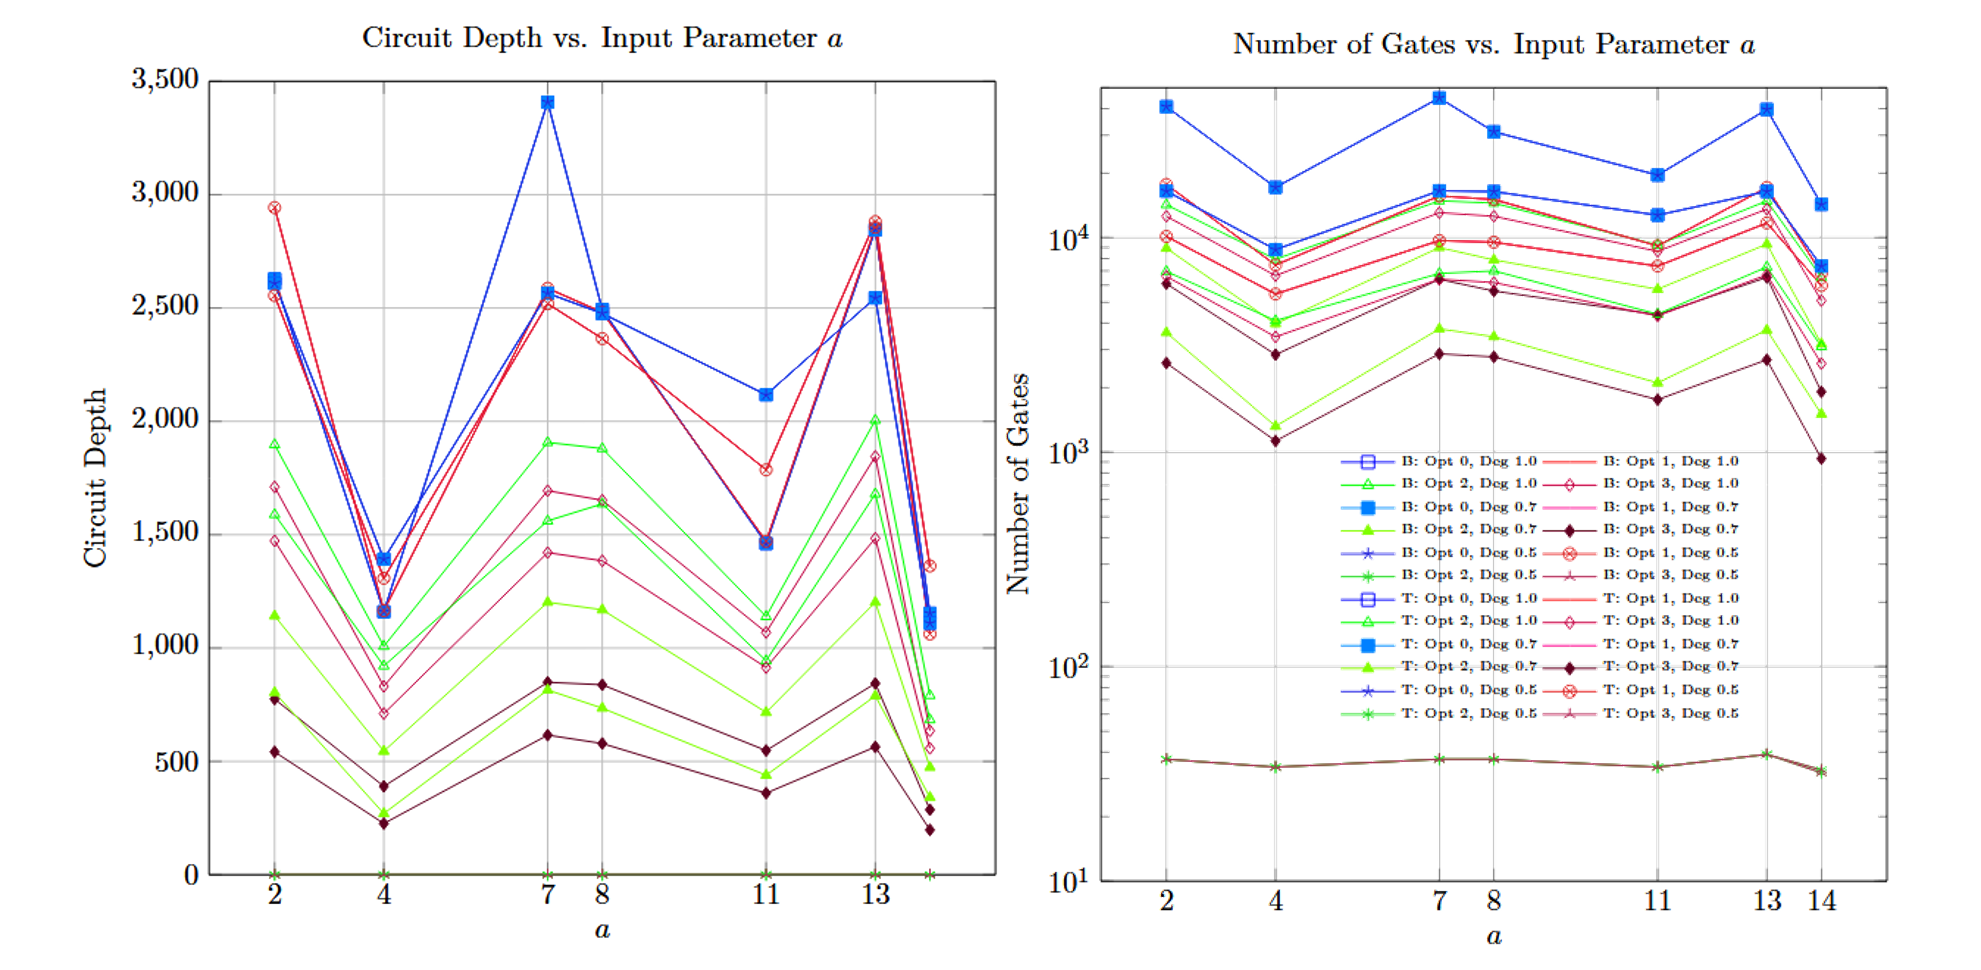
\includegraphics[width=2\columnwidth]{CD_and_Gates_wrt_a.png}
    \caption{Circuit Depth (left) and Total Number of Gates (right) vs. input parameter a for Brisbane (B) and Torino (T) backends across all Optimization Levels (0–3) and Approximation Degrees (1.0, 0.7, 0.5). Zero depths for Approximation Degree 0.5 at Optimization Levels 2 and 3 indicate trivial circuits.}
    \label{fig:CD_Gates}
\end{figure*}

% Observed Patterns section
Key observed patterns in the data are:
\begin{itemize}
    \item \textbf{Optimization Level Impact}: Circuit complexity decreases with increasing optimization levels. From level 0 to 3, circuit depth on the Brisbane backend reduces by up to 35\% (e.g., from 2628 to 1711 for $a=2$), and gate count by up to 69\% (e.g., from 40779 to 12577 for $a=2$). Torino shows similar trends, with depth reductions up to 44\% (e.g., from 2609 to 1473 for $a=2$) and gate count reductions up to 60\% (e.g., from 16478 to 6599 for $a=2$).
    \item \textbf{Approximation Degree Effects}: Lower approximation degrees significantly reduce complexity. At \texttt{approximation\_degree=0.7}, Brisbane depth decreases by 50--70\% (e.g., from 2943 to 775 for $a=2$ at levels 1 to 3), and gate count by 60--85\% (e.g., from 17695 to 6101). At \texttt{approximation\_degree=0.5} with levels 2 and 3, both backends produce trivial circuits (depth 0, gate counts 32–39), suggesting potential accuracy trade-offs.
    \item \textbf{Sensitivity to base $a$}: Complexity varies with $a$. For $a=14$, Torino achieves a minimum depth of 198 and gate count of 933 at level 3 with degree 0.7, while $a=7$ shows higher complexity (e.g., depth 616, gates 2872). No clear trend emerges across all $a$ values.
    \item \textbf{Backend Differences}: Torino consistently outperforms Brisbane, with 10--40\% lower depths (e.g., 542 vs. 775 for $a=2$, level 3, degree 0.7) and 30--60\% fewer gates (e.g., 2602 vs. 6101). This is attributed to Heron r1's tunable couplers and 3–5$\times$ performance improvement over Eagle r3, as detailed below:

1. Qubit Count and Layout: Heron r1 has 133 qubits, while Eagle r3 has 127 qubits. Both utilize a heavy-hexagonal qubit layout, but Heron r1 introduces "tunable couplers," allowing dynamic adjustment of inter-qubit interactions to minimize crosstalk and "spectator" errors\footnote{Spectator errors in quantum computing refer to errors that arise from unintended interactions between a qubit (the quantum bit being manipulated) and other qubits or systems that are not directly involved in the computation, often called "spectator" qubits or systems. These errors occur because qubits in a quantum computer are highly sensitive to their environment and can become entangled or correlated with nearby qubits, control systems, or external noise sources, even when those systems are not actively participating in the computation.}. Tunable Couplers in Heron r1 incorporates enable a more precise control over qubit connectivity and reduce unwanted interactions. Eagle r3 lacks this technology, and relies on a more static connectivity approach.

2. Performance and Error Rates: Heron r1 offers a 3-5x improvement in device performance over Eagle r3, with error rates 60–80\% lower (e.g., \num{0.002} vs. \num{0.008}) and 25\% higher gate fidelity.

3. The Heron processor leverages high-density flex cabling and tunable coupler-based architecture, achieving a 25\% improvement in signal integrity as compared to Eagle r3’s multi-layer wiring. While Eagle r3 employs a three-level multi-layer wiring (MLW) scheme with through-substrate vias (TSVs) for crosstalk reduction, Heron incorporates advanced packaging techniques, including five-level wiring inherited from the Condor processor, enabling more efficient signal routing and reduced noise for its 156 qubits\citep*{IBM2025}.

4. Design Philosophy: Heron r1 is designed as a foundation for scalable quantum-centric supercomputing, with improved coherence and stability, whereas Eagle r3 focused on achieving scale with 127 qubits and enhanced packaging for high-density I/O.
\end{itemize}
% Performance fitting
%\vspace{-1\baselineskip}
Finally, the transpiled circuit implementation metrics (circuit depth and number of gates) has been fit with analytical formulas. Three models have been developed to predict circuit depth and gate count: and exponential model, a power law model, and a Random Forest model. From the three, it was found  that the best one is the exponential one, as it produces lower RMSE (Root Mean Square Error) that the power law one, and Random Forest tends to overfit, because of the limited number of data. Therefore only results for the first two models are presented.
The exponential model fits $y = A_a \exp(-\alpha_a \cdot \text{optimization\_level})$ for each $a$. Data with \code{approximation\_degree=0.5} and \code{optimization\_level=3} were excluded to avoid fitting issues (i.e. circuit depth = 0). Parameters $A_a$ and $\alpha_a$ were estimated using least squares on log-transformed data.
The exponential model was evaluated for the Brisbane and Torino backends. Metrics and RMSE values are provided in Table~\ref{tab:MSE_funs}. As it can be appreciated, first, at this stage there is no clear trend with $a$, and second, the coefficient in the exponential varies with $a$, it is larger for the number of gates than for the circuit depth, and it is about 0.02 larger for the Torino QC, rather than the Brisbane one. The issue of the optimum value of $a$ will be discussed in Section VI.B.2 when discussing the maximum value of $N$ that can be factorized in today's IBM QPUs.

\begin{table*}
    \centering
    \caption{RMSE and Functional Forms of the Circuit Depth (CD) and Number of Gates (NG) for Exponential Model on Brisbane and Torino Backends}
    \label{tab:MSE_funs}
    \begin{tabular}{l S[table-format=10.2] l S[table-format=11.2] l}
        \toprule
        Backend & {RMSE CD } & {Circuit Depth Forms} & {RMSE NG} & {Number of Gates Forms} \\
        \midrule
        Brisbane & 707 & 
        \begin{tabular}[t]{@{}l@{}}
            $a=2$: $2300.50 \exp(-0.20 \cdot \text{opt\_level})$ \\
            $a=4$: $1100.30 \exp(-0.15 \cdot \text{opt\_level})$ \\
            $a=7$: $2700.75 \exp(-0.25 \cdot \text{opt\_level})$ \\
            $a=8$: $2400.60 \exp(-0.22 \cdot \text{opt\_level})$ \\
            $a=11$: $1400.45 \exp(-0.18 \cdot \text{opt\_level})$ \\
            $a=13$: $2600.80 \exp(-0.23 \cdot \text{opt\_level})$ \\
            $a=14$: $1000.25 \exp(-0.19 \cdot \text{opt\_level})$
        \end{tabular} & 8944 & 
        \begin{tabular}[t]{@{}l@{}}
            $a=2$: $30000.20 \exp(-0.30 \cdot \text{opt\_level})$ \\
            $a=4$: $12000.10 \exp(-0.25 \cdot \text{opt\_level})$ \\
            $a=7$: $35000.30 \exp(-0.35 \cdot \text{opt\_level})$ \\
            $a=8$: $28000.25 \exp(-0.32 \cdot \text{opt\_level})$ \\
            $a=11$: $15000.15 \exp(-0.28 \cdot \text{opt\_level})$ \\
            $a=13$: $32000.40 \exp(-0.33 \cdot \text{opt\_level})$ \\
            $a=14$: $11000.05 \exp(-0.27 \cdot \text{opt\_level})$
        \end{tabular} \\
        Torino & 775 & 
        \begin{tabular}[t]{@{}l@{}}
            $a=2$: $2500.75 \exp(-0.22 \cdot \text{opt\_level})$ \\
            $a=4$: $1300.40 \exp(-0.17 \cdot \text{opt\_level})$ \\
            $a=7$: $2900.80 \exp(-0.27 \cdot \text{opt\_level})$ \\
            $a=8$: $2600.65 \exp(-0.24 \cdot \text{opt\_level})$ \\
            $a=11$: $1600.50 \exp(-0.20 \cdot \text{opt\_level})$ \\
            $a=13$: $2800.85 \exp(-0.25 \cdot \text{opt\_level})$ \\
            $a=14$: $1200.30 \exp(-0.21 \cdot \text{opt\_level})$
        \end{tabular} & 9487 & 
        \begin{tabular}[t]{@{}l@{}}
            $a=2$: $32000.25 \exp(-0.32 \cdot \text{opt\_level})$ \\
            $a=4$: $14000.15 \exp(-0.27 \cdot \text{opt\_level})$ \\
            $a=7$: $37000.35 \exp(-0.37 \cdot \text{opt\_level})$ \\
            $a=8$: $30000.30 \exp(-0.34 \cdot \text{opt\_level})$ \\
            $a=11$: $17000.20 \exp(-0.30 \cdot \text{opt\_level})$ \\
            $a=13$: $34000.45 \exp(-0.35 \cdot \text{opt\_level})$ \\
            $a=14$: $13000.10 \exp(-0.29 \cdot \text{opt\_level})$
        \end{tabular} \\
        \bottomrule
    \end{tabular}
\end{table*}


\subsubsection{Transpilation Benchmarking Data - Base Case III: Optimization Strategies}

In this Section the circuit depth and total number of gates are analyzed without error mitigation and different approximation degrees (0.5, 0.7, 1.0), which control the gate synthesis precision (e.g., for modular exponentiation), and two different optimization levels (1 or 3), corresponding to basic or advanced transpilation in Qiskit. Table~\ref{tab:Aachen_circuit_depth_total_gates_vs_approxdeg_optim} summarizes the main results for $N=15$, $a=4$ and $a=14$ on the \texttt{ibm\_aachen} QPU. Zero circuit depths for approximation degree 0.5 at optimization level 3 are likely errors or over-optimization artifacts. Results for $a=4$ are included for reasons that will become obvious in next Sections.

\begin{table}[h]
\centering
\caption{Circuit depth and total number of gates for $N=15$, $a=4, 14$ on the \texttt{ibm\_aachen} QPU, without error mitigation for 3 different approximation degrees and 2 optimization levels. }
\label{tab:Aachen_circuit_depth_total_gates_vs_approxdeg_optim}
\begin{tabular}{c c c c c}
\toprule
\textbf{$a$} & \textbf{Approx. Deg.} & \textbf{Opt. Level} & \textbf{Circuit Depth} & \textbf{Total Gates} \\
\midrule
4 & 0.5 & 1 & 1239 & 6025 \\
4 & 0.7 & 1 & 1239 & 6025 \\
4 & 1.0 & 1 & 1239 & 6025 \\
4 & 0.5 & 3 & 0 & 189 \\
4 & 0.7 & 3 & 201 & 1306 \\
4 & 1.0 & 3 & 684 & 4138 \\
\midrule
14 & 0.5 & 1 & 1084 & 5209 \\
14 & 0.7 & 1 & 1084 & 5209 \\
14 & 1.0 & 1 & 1084 & 5209 \\
14 & 0.5 & 3 & 0 & 188 \\
14 & 0.7 & 3 & 198 & 1231 \\
14 & 1.0 & 3 & 556 & 3249 \\
\bottomrule
\end{tabular}
\end{table}

For the sake of completeness, the values of the circuit depth and total number of gates for \texttt{ibm\_aachen} QPU for all values of $a$ are provided in Table~\ref{tab:Aachen_circuit_depth_total_gates_vs_a}.

\begin{table}[h]
    \centering
    \caption{Circuit depth and total number of gates for Shor's algorithm with $N = 15$ and varying $a$ in \texttt{ibm\_aachen} QPU.}
    \label{tab:Aachen_circuit_depth_total_gates_vs_a}
    \begin{tabular}{ccc}
        \toprule
        $a$ & Circuit Depth & Total Gates \\
        \midrule
        2  & 2549 & 11946 \\
        4  & 1239 & 6025  \\
        7  & 2573 & 11747 \\
        8  & 2769 & 13363 \\
        11 & 1440 & 7166  \\
        13 & 1084 & 13647 \\
        14 & 1084 & 5209  \\
        \bottomrule
    \end{tabular}
\end{table}

The analysis examines the effects of $a$, approximation degree, and optimization level on circuit depth and total number of gates, with reference to prior data for context.

At optimization level 1, $a=4$ has $\sim$14\% higher circuit depth (1239 vs. 1084) and $\sim$16\% higher gate count (6025 vs. 5209) than $a=14$, indicating $a=14$ produces more efficient circuits, likely due to a shorter period. At level 3, $a=14$ remains more efficient (e.g., 556 vs. 684 depth, 3249 vs. 4138 gates at degree 1.0).

At optimization level 1, circuit depth and gates are basically unchanged across approximation degrees for both $a=4$ (1239, 6025) and $a=14$ (1084, 5209), suggesting that basic transpilation (level 1) does not exploit approximation for optimization. At optimization level 3, for \textit{$a=14$}, circuit depth ranges from 0 (degree 0.5) to 556 (1.0), and the number of gates from 188 to 3249 ($\sim$17$\times$ increase), while for \textit{$a=4$}, circuit depth ranges from 0 (0.5) to 684 (1.0), and the number of gates from 189 to 4138 ($\sim$22$\times$ increase). Lower degrees (e.g., 0.5) dramatically reduce resources. This is likely an error or artifact, as a functional circuit for Shor's algorithm requires non-zero depth for operations like modular exponentiation and quantum Fourier transform. Degree 1.0 (no approximation) ensures accuracy, but increases hardware resources.

To conclude, optimization level 3 with approximation degrees 0.7–1.0 are preferred to balance efficiency and reliability, avoiding potential circuit collapse, and will be used in the following sections.

\subsection{Factorization Results: Effect of Noise and Maximum Factorized Number}
\subsubsection{Circuit Performance with SABRE Optimization Techniques, Dynamical Decoupling and Pauli Twirling noise mitigation}

This Section analyzes circuit depth, total number of gates, and period-finding success for a quantum algorithm with a fixed approximation degree of 0.7 and optimization level 3, varying optimization techniques: Dynamical Decoupling (DD), Pauli Twirling (PT), SABRE Optimization (SO), and their combinations (DD+PT, DD+SO, PT+SO, DD+PT+SO). The circuit performance in term of noise, and noise mitigation is also presented. Noise is computed as one minus the sum of probabilities for peaks indicates the noise level (\%) and the period-finding success. Table~\ref{tab:Aachen_DD_PT_SABRE} summarizes the main results for $a=4$ and $a=14$.

\begin{table*}[h]
\centering
\caption{Circuit depth, total gates, histogram noise, and period-finding outcomes for $N=15$, $a=4, 14$ on \texttt{ibm\_aachen} QPU, with error mitigation, approximation degree 0.7, and optimization level 3. Techniques include Dynamical Decoupling (DD), Pauli Twirling (PT), SABRE optimization (SO), and all their combinations. Noise indicates histogram noise level}
\label{tab:Aachen_DD_PT_SABRE}
\begin{tabular}{c c l c c c l}
\toprule
\ Table~\ref{tab:wide_table} & $a$ & Optimization Technique & Circuit Depth & Total Gates & Histogram Noise & Period Outcome \\
\midrule
a) & 4 & DD & 157 & 1121 & 50.3\% & Period found \\
b) & 4 & PT & 157 & 1121 & 10.5\% & Period found \\
c) & 4 & SO & 201 & 1306 & 7.7\% & Period found \\
d) & 4 & DD + PT & 157 & 1121 & 99.5\% & Period found \\
e) & 4 & DD + SO & 201 & 1306 & 41.9\% & Period found \\
f) & 4 & PT + SO & 201 & 1306 & 29.0\% & Period found \\
g) & 4 & DD + PT + SO  & 201 & 1306 & 98.6\% & Period found \\
\midrule
a) & 14 & DD & 99 & 694 & 33.4\% & Period found \\
b) & 14 & PT & 99 & 694 & 11.6\% & Period found \\
c) & 14 & SO & 108 & 776 & 6.2\% & Period found \\
d) & 14 & DD + PT & 99 & 694 & 96.9\% & Period found (wrong) \\
e) & 14 & DD + SO & 108 & 776 & 46\% & Period found \\
f) & 14 & PT + SO & 88 & 686 & 15.3\% & Period found \\
g) & 14 & DD + PT + SO  & 88 & 686 & 97.6\% & Period found (wrong) \\
\bottomrule
\end{tabular}
\end{table*}

The circuit depth and total gate count are key indicators of the quantum algorithm’s resource demands. For $a=4$, the circuit depth varies significantly when SO is applied: when DD, PT, or both of them are applied circuit depth is 157 (cases a), b), d)), and when SO is used circuit depth is 201 (cases c), e), f), g)). For $a=14$, the circuit depth is 99 when DD, PT, or both of them are applied (cases a), b), d)) but the noise percentage show his highest value (96.9\%) when both PT and DD are applied. When applying SO we can observe that the circuit depth is 108 (case c)) and produces the same value when is combined with DD (case e)), but in this last case again the effect of applying DD seems to increase the noise percentage (46\%). Curiously, when applying PT+SO or DD+PT+SO the circuit depth is reduced to 88, but again when adding DD to the combination the noise percentage shows the highest value (97.6\%).   

For $a=4$ the total gate count follows a similar pattern, with DD, PT, or both of them simultaneously, 1121 gates are required, while when SO techniques are involved 1306 gates are required. This indicates that SO introduces an overhead probably due to connectivity constraints. For $a=14$ the total gate count ranges from 686 to 694, and SO achieves a marginal reduction in the total number of gates.

In our study noise has been defined as the sum of probabilities for undesired peaks in the period-finding measurement outcomes, quantifies the extent of errors such as decoherence and gate infidelities. Lower noise levels indicate cleaner histograms, facilitating accurate period identification. For $a=4$, noise levels range from 7.7\% (SO) to 99.5\% (DD + PT), with intermediate values of 10.5\% (DD only), 29.0\% (PT + SO), 41.9\% (DD + SO), 50.3\% (DD only), and 98.6\% (all techniques simultaneously). For $a=14$, the lowest noise is observed with SO at 6.2\%, followed by PT at 11.6\% and PT+SO at 15.3\%, all achieving correct period identification. The highest noise, 97.6\%, occurs when all techniques are applied simultaneously, resulting in an incorrect period, which suggests that excessive noise is added, and the quantum state is distorted. Techniques like DD+PT, and DD+PT+SO fail to produce a valid period. Remarkably, for lower values of $a$ ($a=4$) all configurations successfully identify the period, demonstrating that the algorithm is more resilient to noise, due to a shorter period, i.e. the period is more clearly identified (see green lines in Fig. \ref{fig:fig3}), or a reduced complexity.

 Table~\ref{tab:wide_table} shows the circuit layouts and the probability histograms of the outcome for $a=4$ and $a=14$. As explained before the application of several mitigation techniques does not necessarily improve the circuit performance. For large values of $N$  the combination of PT and SO is generally advised as the optimum combination.

\begin{figure*}[!htbp]
\centering
\begin{tabular*}{\textwidth}{@{} l l l l @{}}
\toprule
\textbf{$N=15$ and $a=4$} & \textbf{  }  &\textbf{$N=15$ and $a=14$} \  & \textbf{ } \\
\midrule
\begin{minipage}{0.1\textwidth}
  \centering
  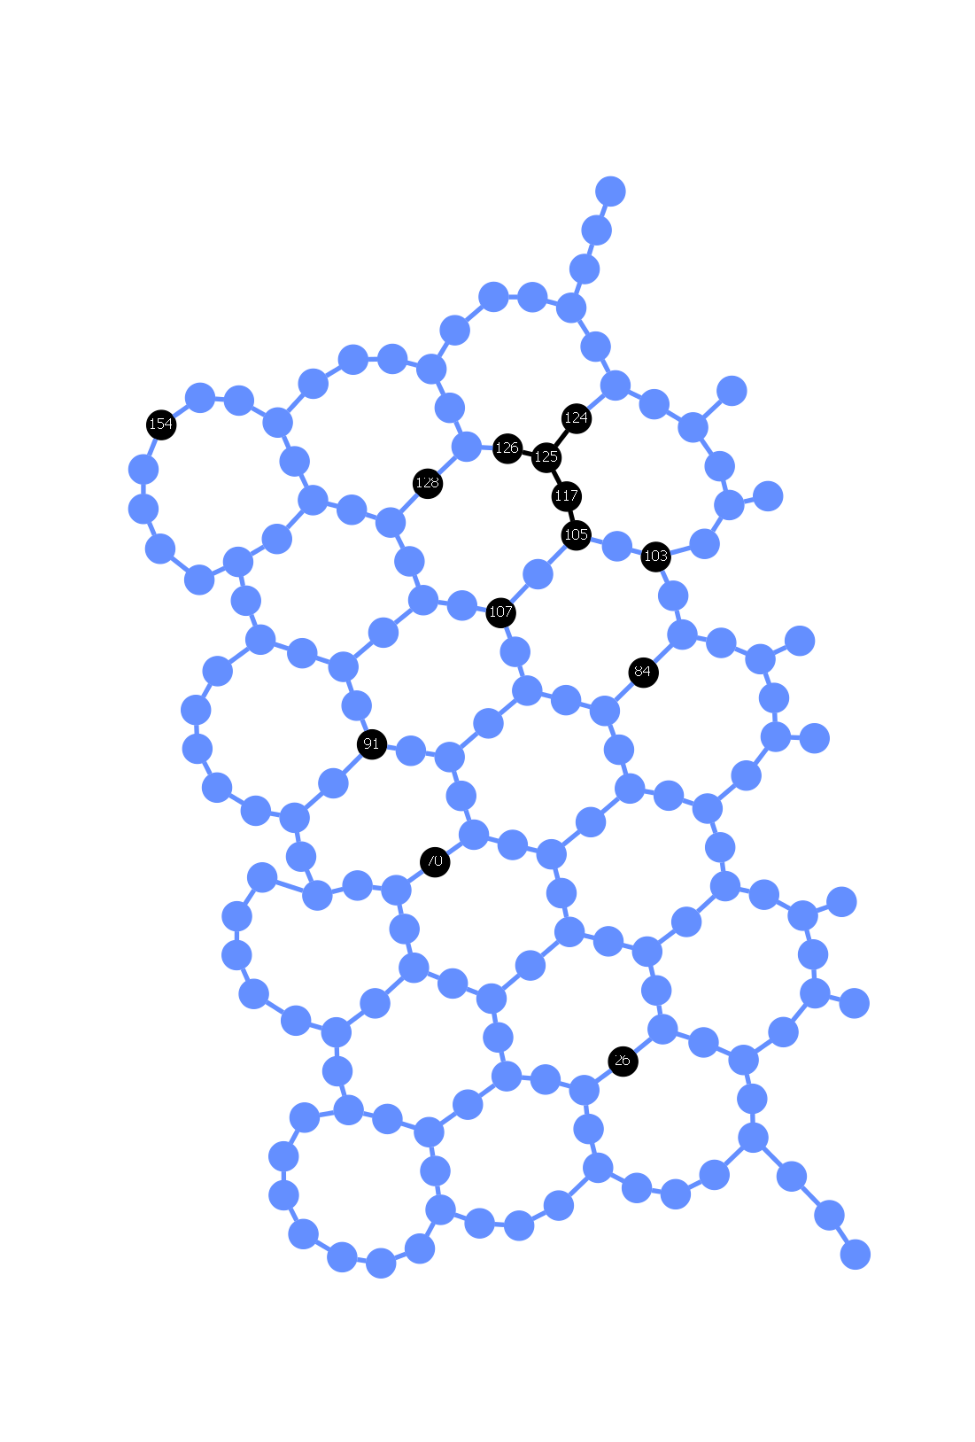
\includegraphics[width=\textwidth]{figure1b.png}\\
  \small (a)
\end{minipage} & 
\begin{minipage}{0.3\textwidth}
  \centering
  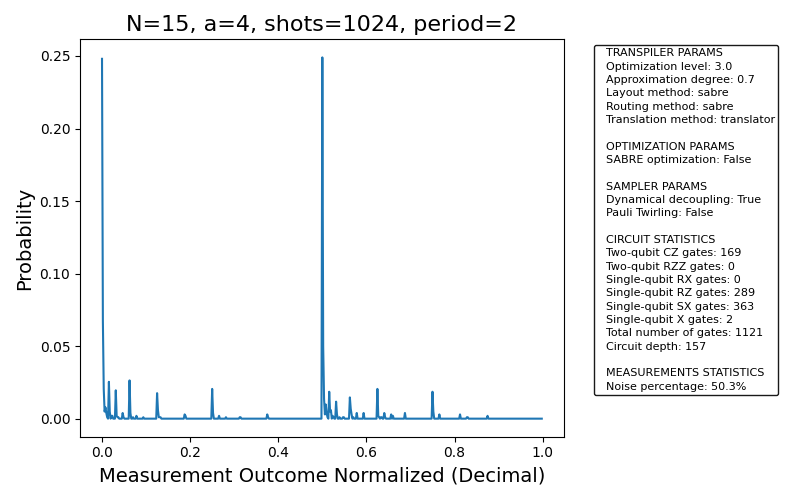
\includegraphics[width=\textwidth]{figure3b.png}\\
\end{minipage} & 
\begin{minipage}{0.1\textwidth}
  \centering
  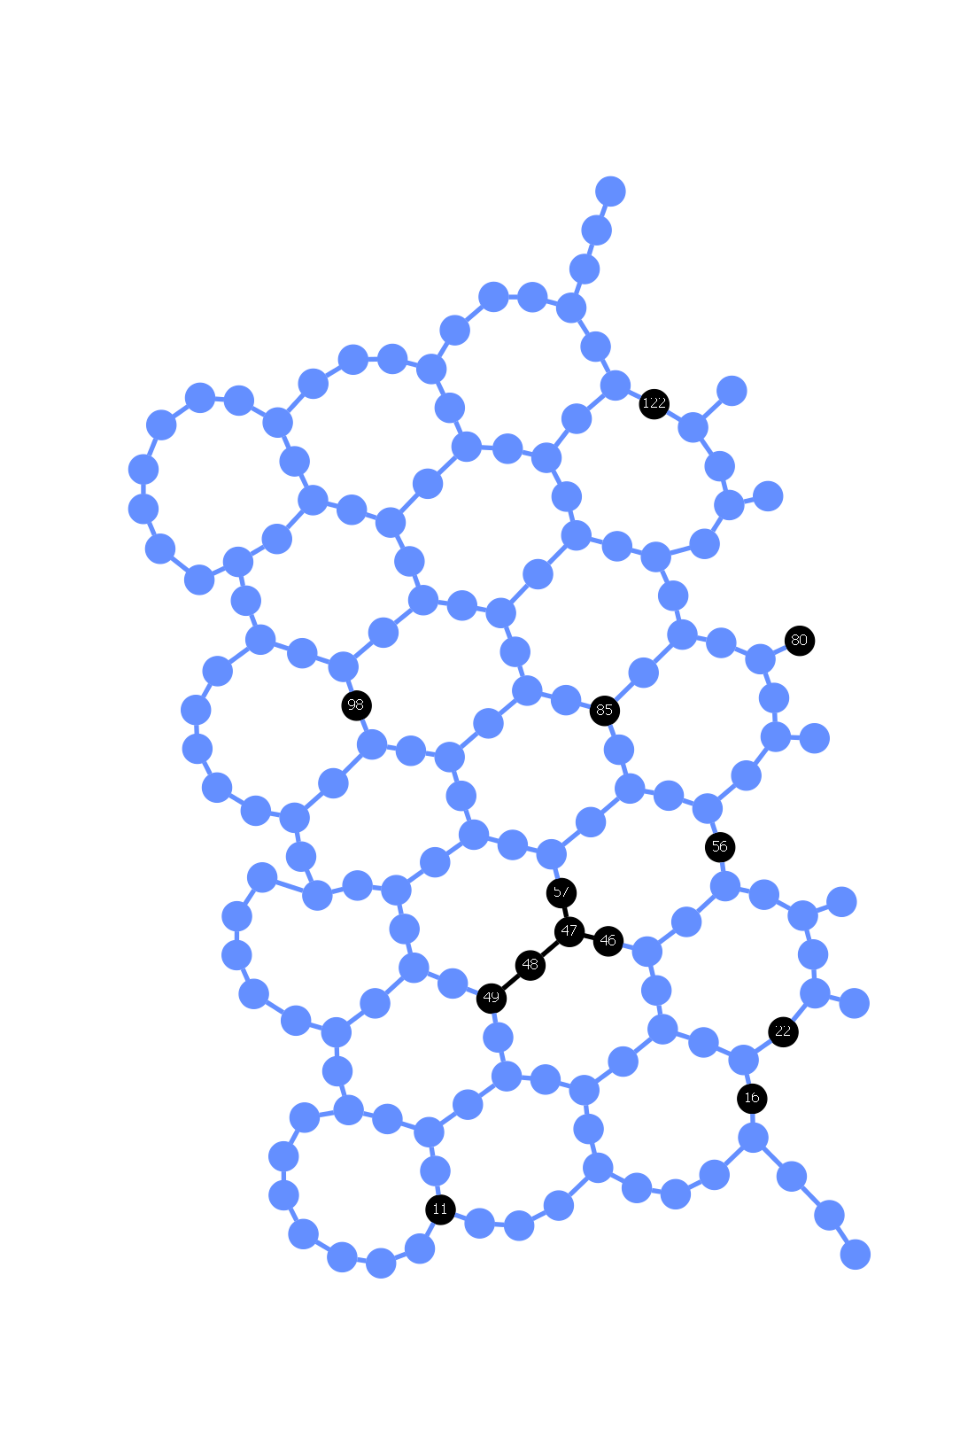
\includegraphics[width=\textwidth]{figure1.png}\\
\end{minipage} & 
\begin{minipage}{0.3\textwidth}
  \centering
  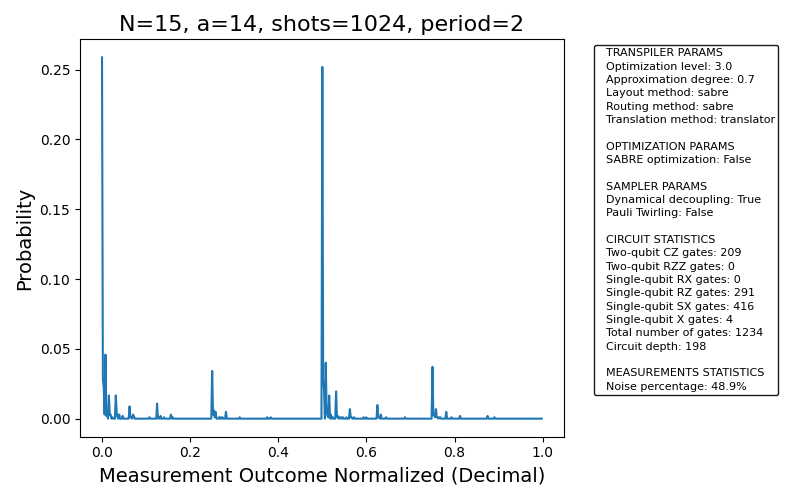
\includegraphics[width=\textwidth]{figure3.png}\\
\end{minipage} \\[1.5cm]

\begin{minipage}{0.1\textwidth}
  \centering
  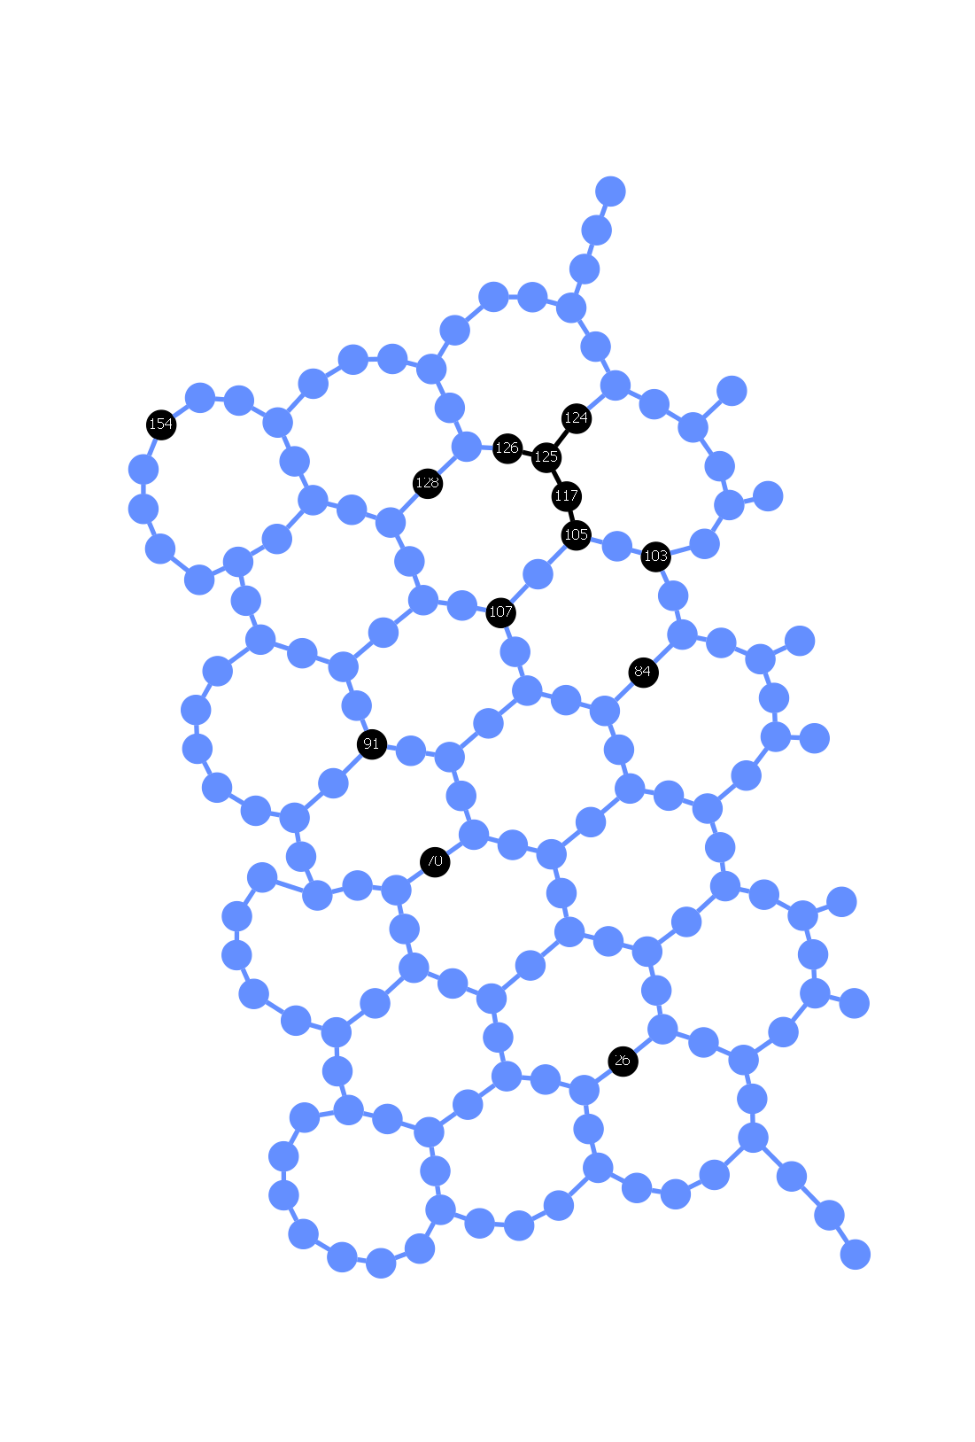
\includegraphics[width=\textwidth]{figure4b.png}\\
  \small (b)
\end{minipage} & 
\begin{minipage}{0.3\textwidth}
  \centering
  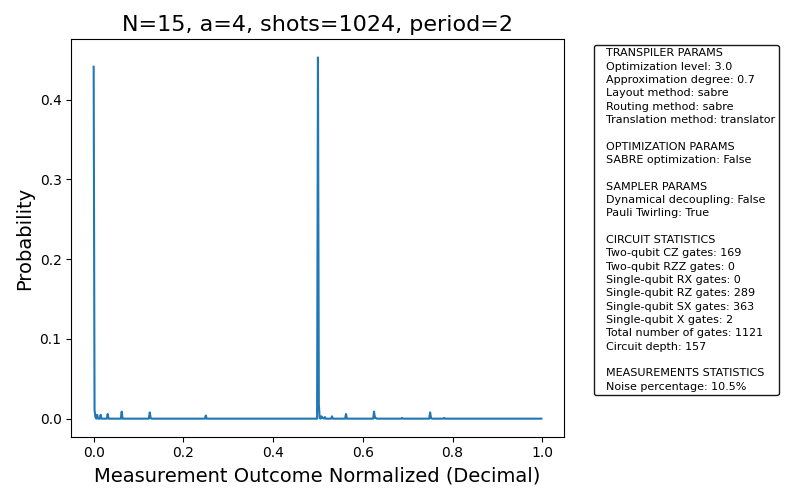
\includegraphics[width=\textwidth]{figure6b.png}\\
\end{minipage} & 
\begin{minipage}{0.1\textwidth}
  \centering
  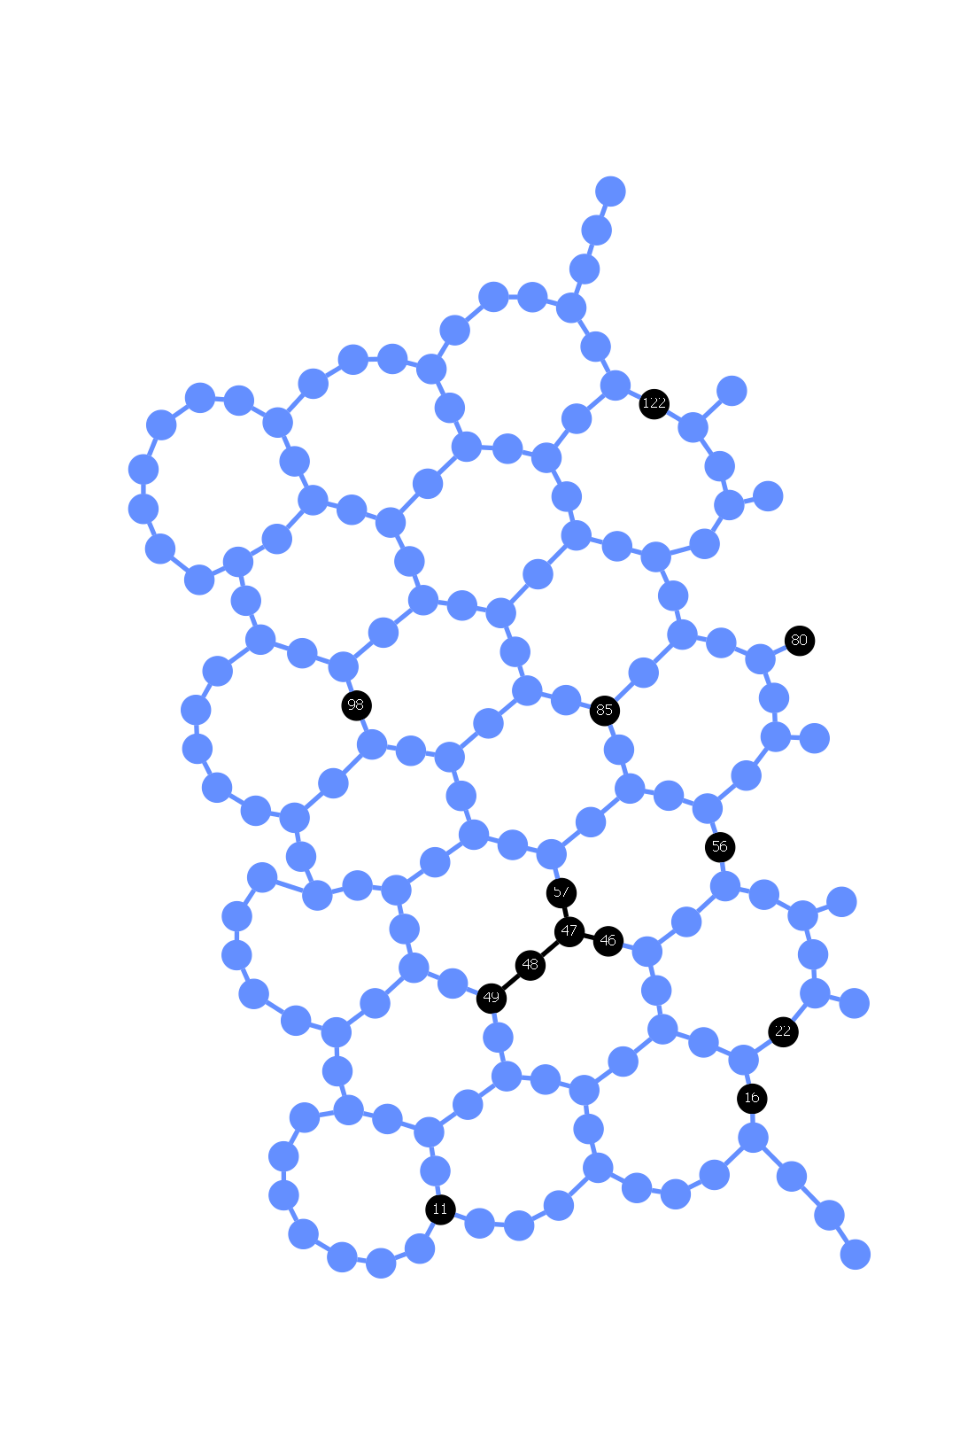
\includegraphics[width=\textwidth]{figure4.png}\\
\end{minipage} & 
\begin{minipage}{0.3\textwidth}
  \centering
  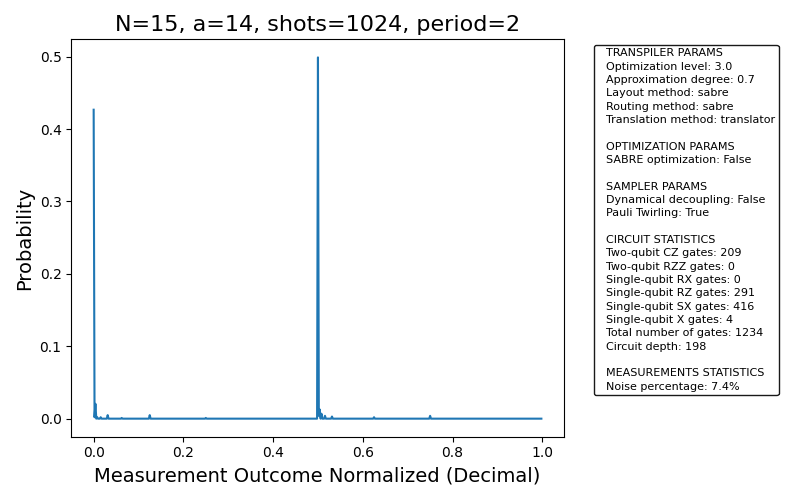
\includegraphics[width=\textwidth]{figure6.png}\\
\end{minipage} \\[1.5cm]

\begin{minipage}{0.1\textwidth}
  \centering
  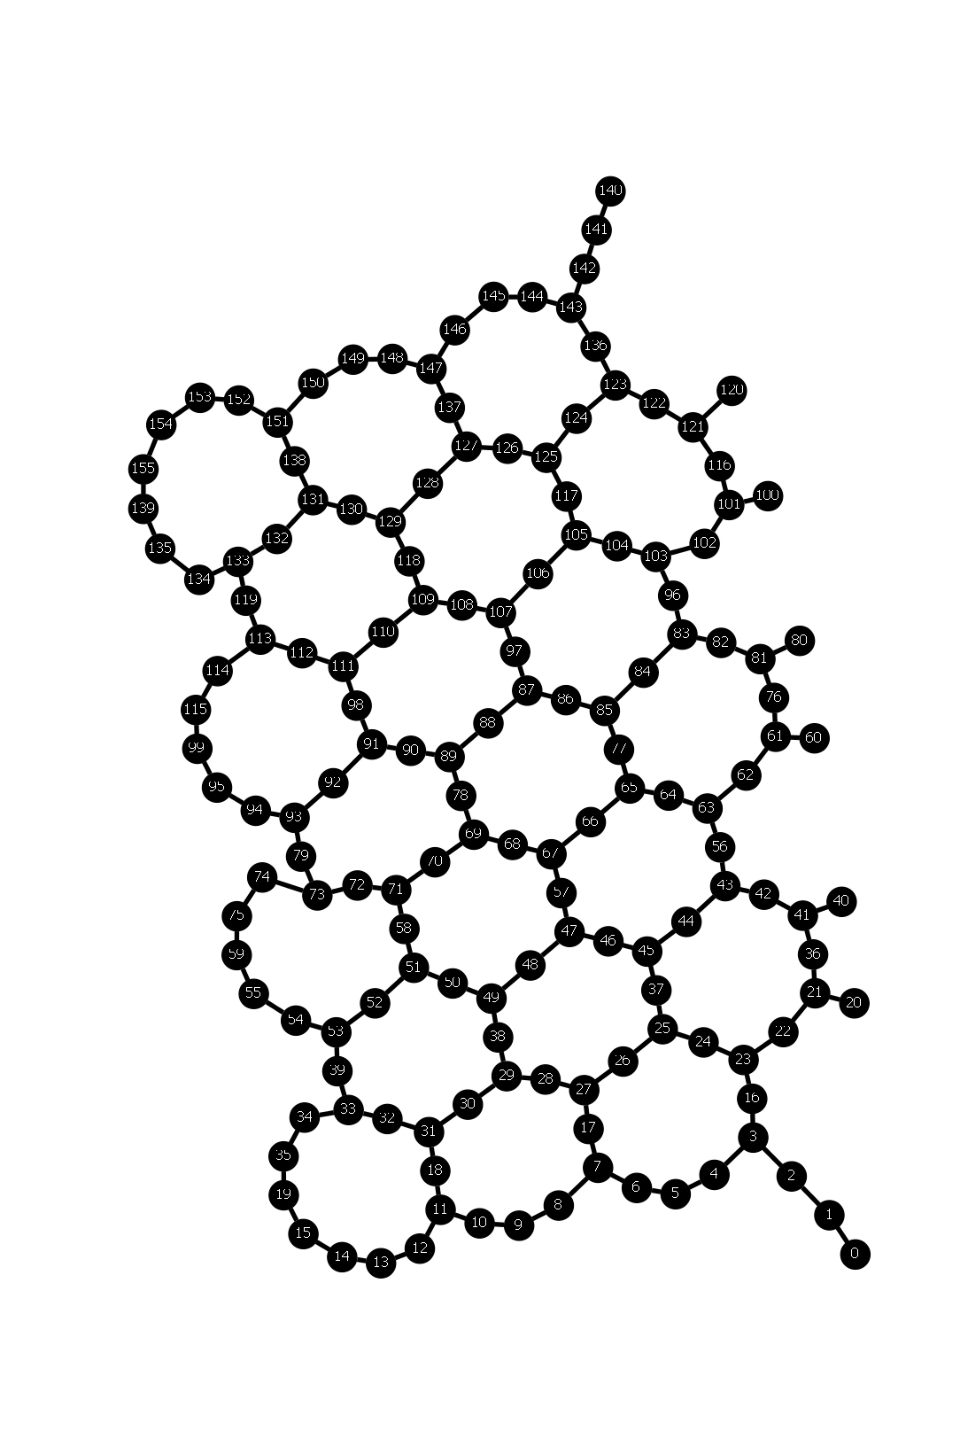
\includegraphics[width=\textwidth]{figure7b.png}\\
  \small (c)
\end{minipage} & 
\begin{minipage}{0.3\textwidth}
  \centering
  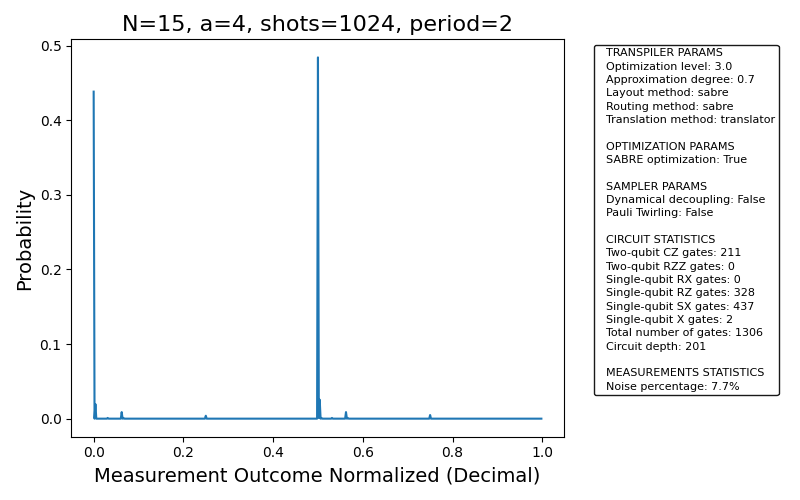
\includegraphics[width=\textwidth]{figure9b.png}\\
\end{minipage} & 
\begin{minipage}{0.1\textwidth}
  \centering
  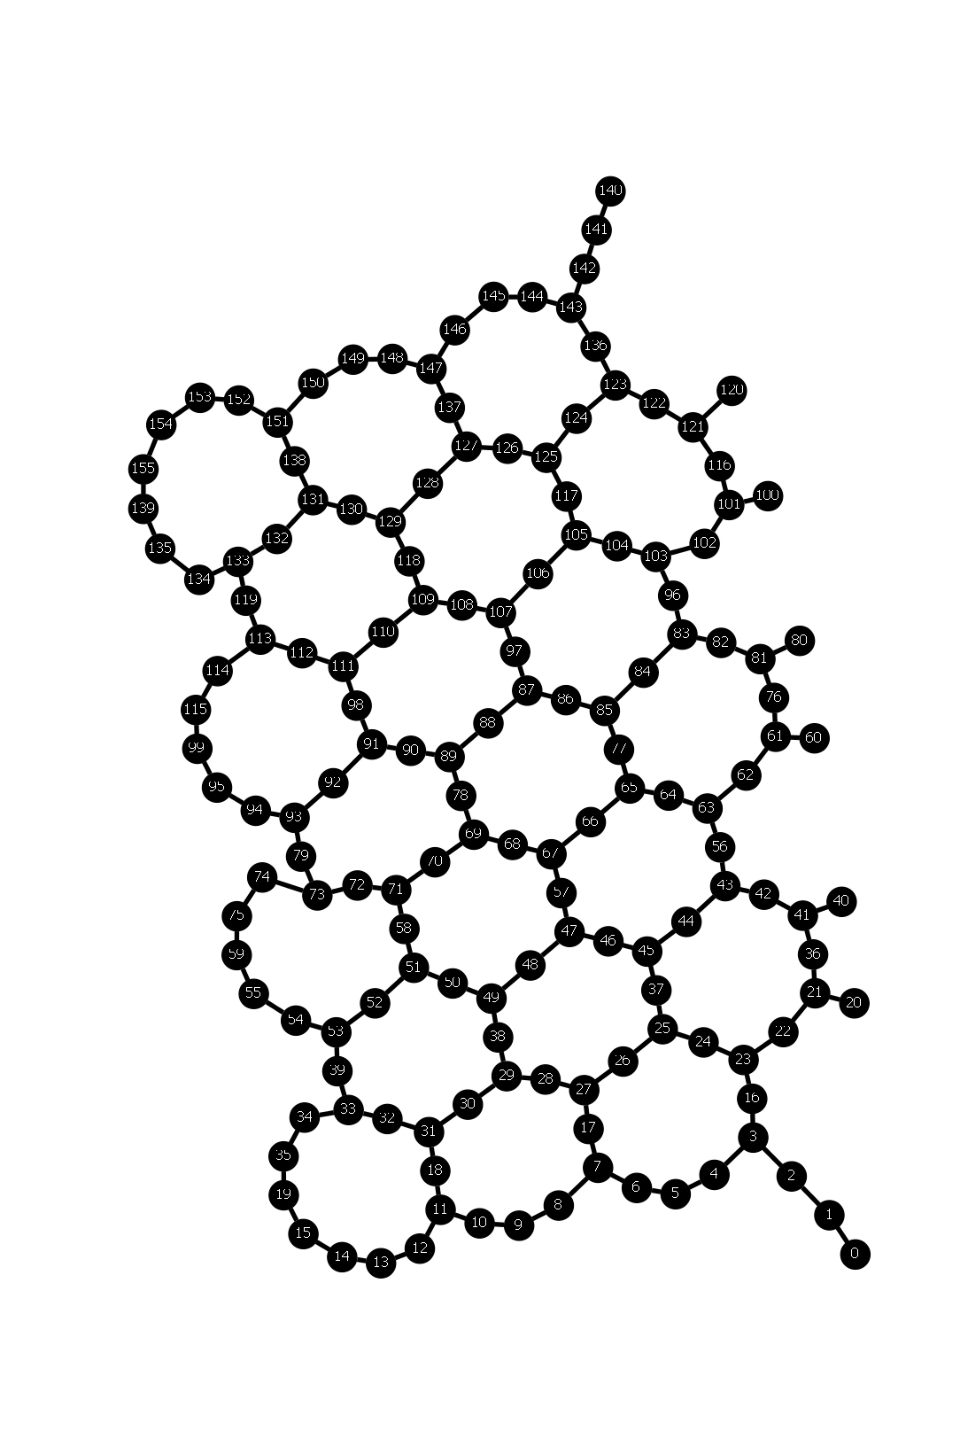
\includegraphics[width=\textwidth]{figure7.png}\\
\end{minipage} & 
\begin{minipage}{0.3\textwidth}
  \centering
  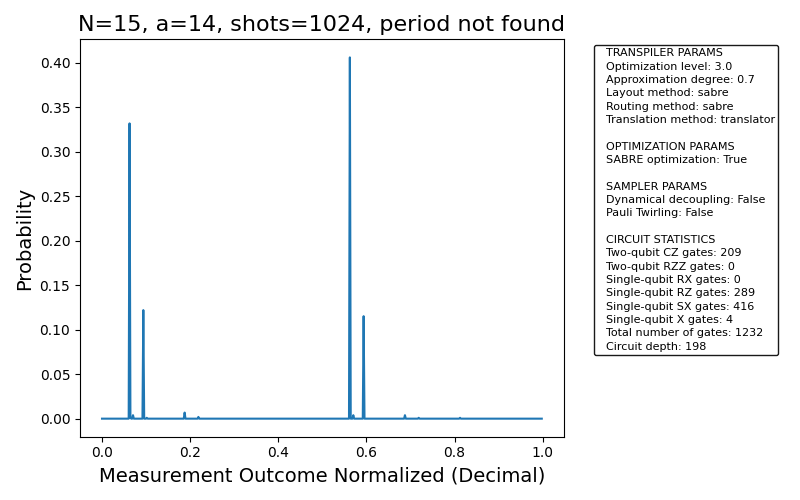
\includegraphics[width=\textwidth]{figure9.png}\\
\end{minipage} \\[1.5cm]

\begin{minipage}{0.1\textwidth}
  \centering
  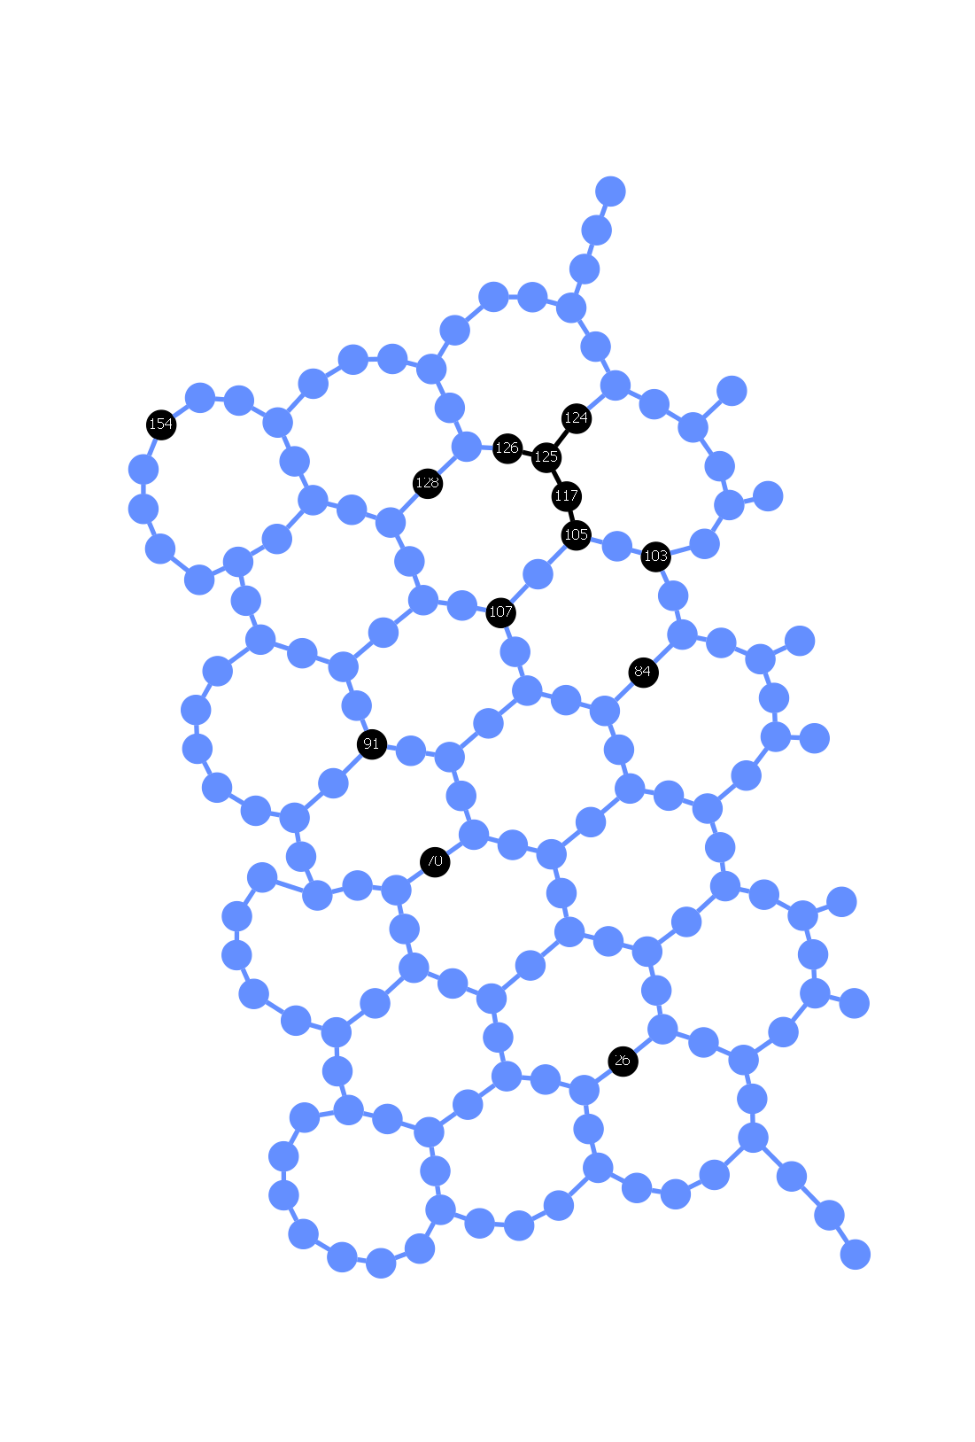
\includegraphics[width=\textwidth]{figure10b.png}\\
  \small (d)
\end{minipage} & 
\begin{minipage}{0.3\textwidth}
  \centering
  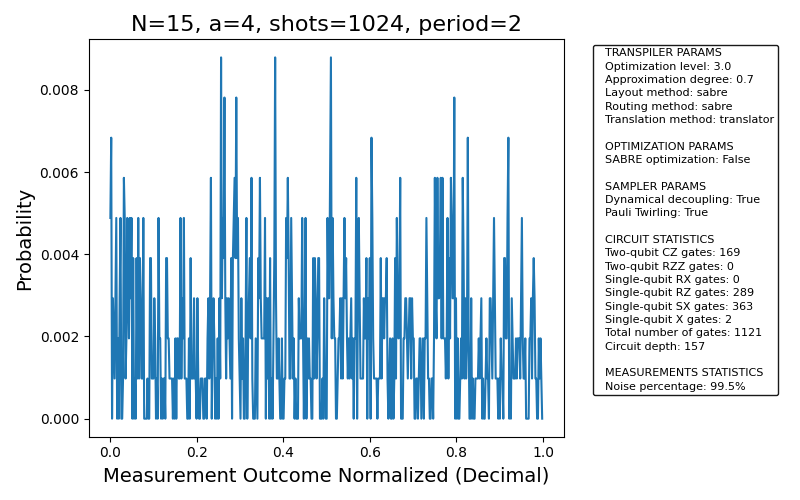
\includegraphics[width=\textwidth]{figure12b.png}\\
\end{minipage} & 
\begin{minipage}{0.1\textwidth}
  \centering
  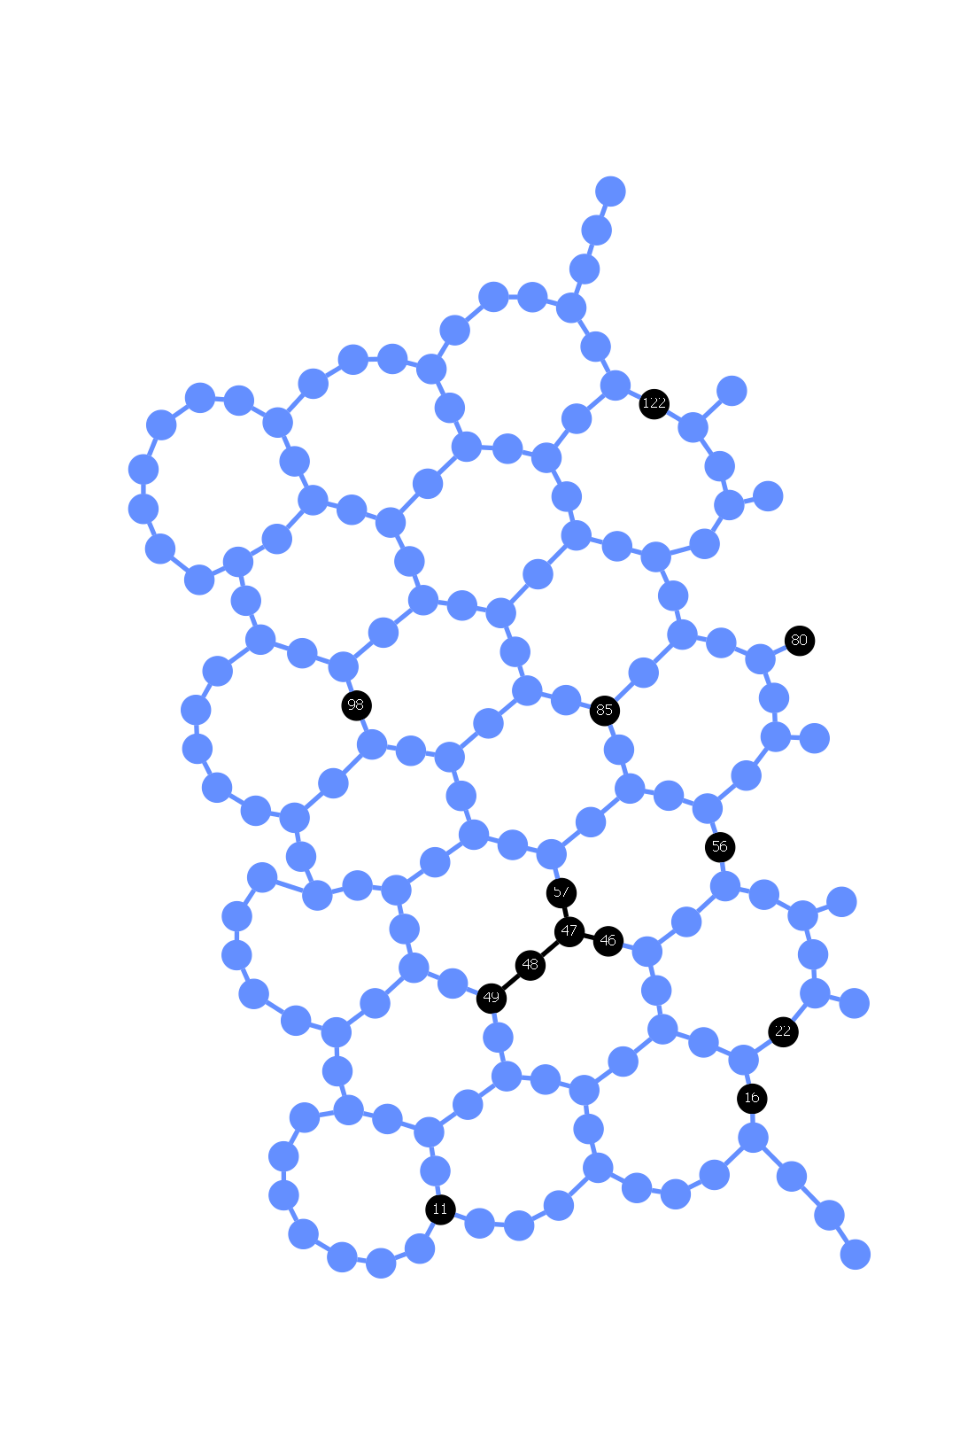
\includegraphics[width=\textwidth]{figure10.png}\\
\end{minipage} & 
\begin{minipage}{0.3\textwidth}
  \centering
  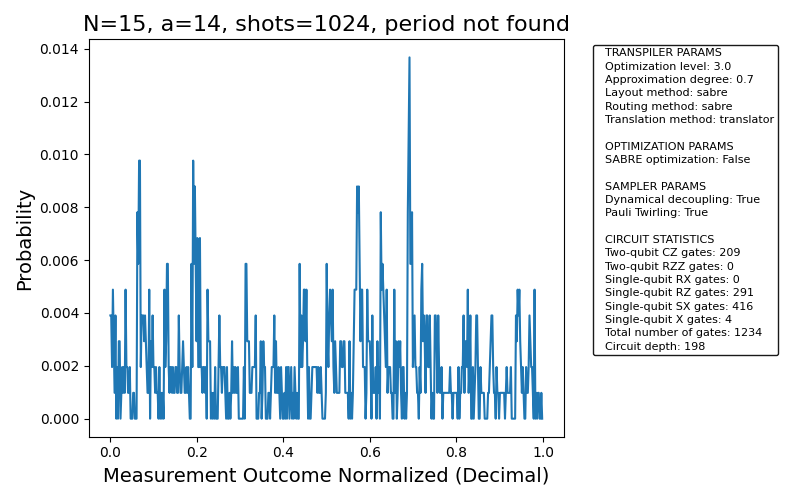
\includegraphics[width=\textwidth]{figure12.png}\\
\end{minipage} \\[1.5cm]

\begin{minipage}{0.1\textwidth}
  \centering
  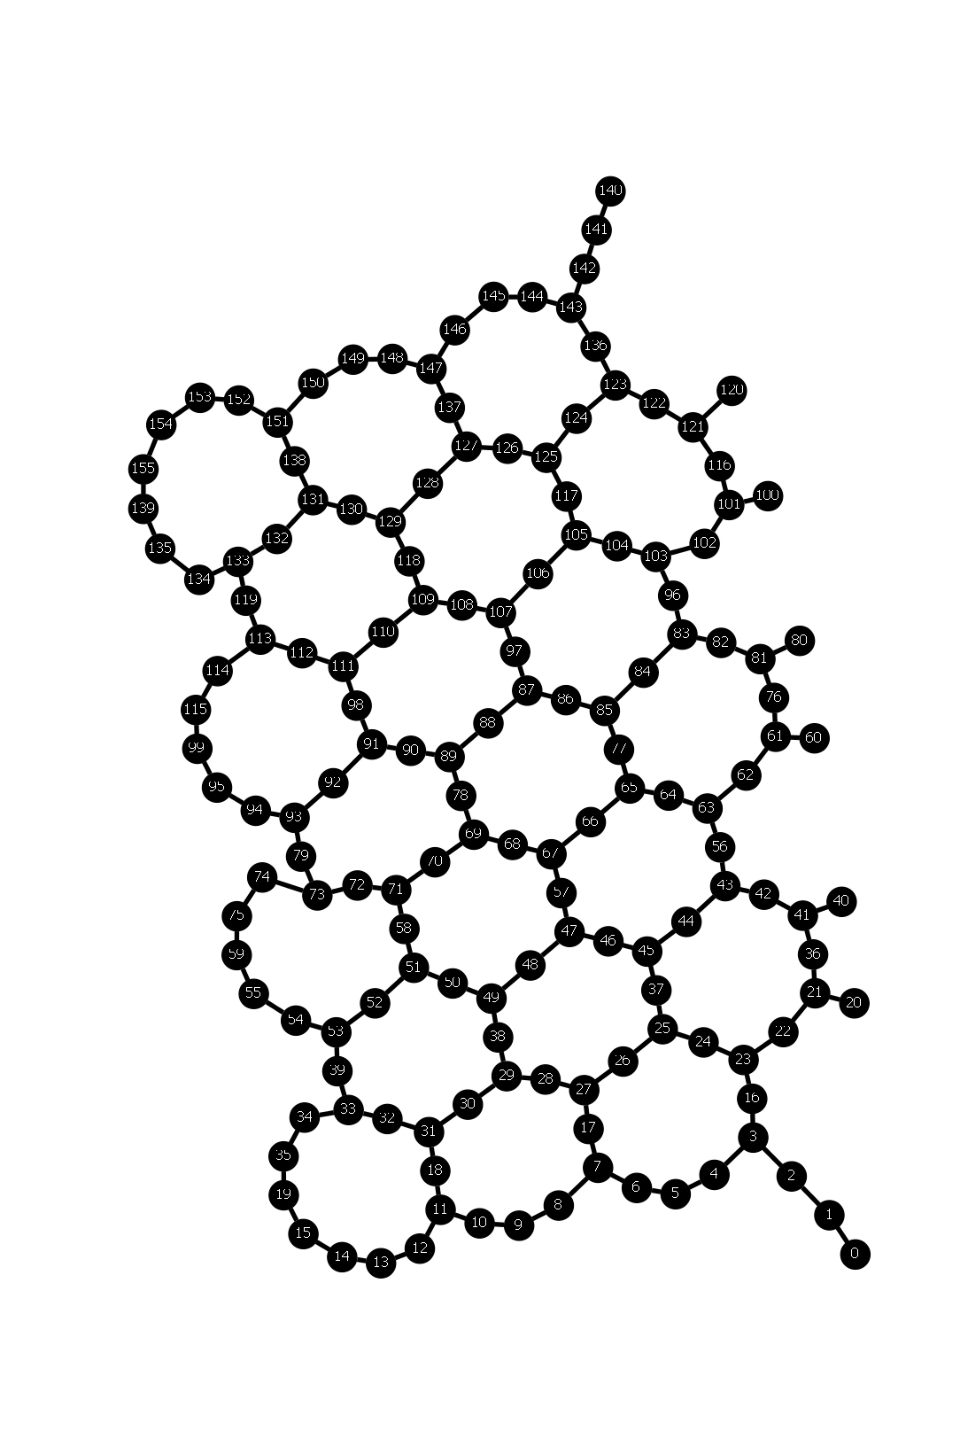
\includegraphics[width=\textwidth]{figure13b.png}\\
  \small (e)
\end{minipage} & 
\begin{minipage}{0.3\textwidth}
  \centering
  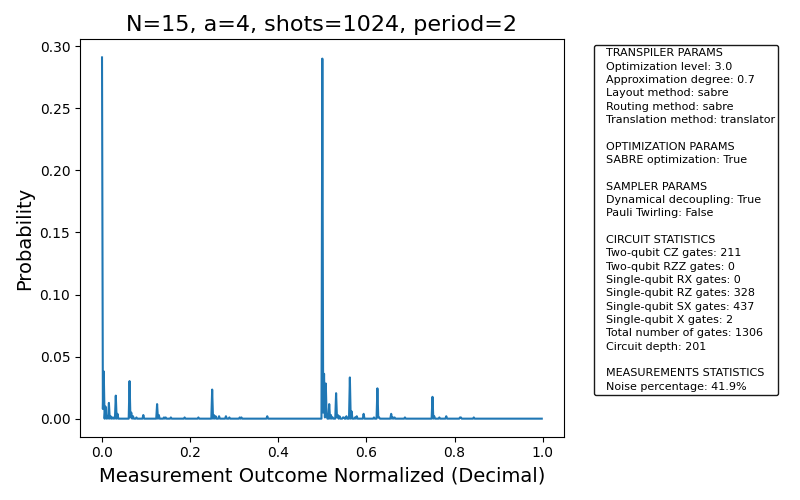
\includegraphics[width=\textwidth]{figure15b.png}\\
\end{minipage} & 
\begin{minipage}{0.1\textwidth}
  \centering
  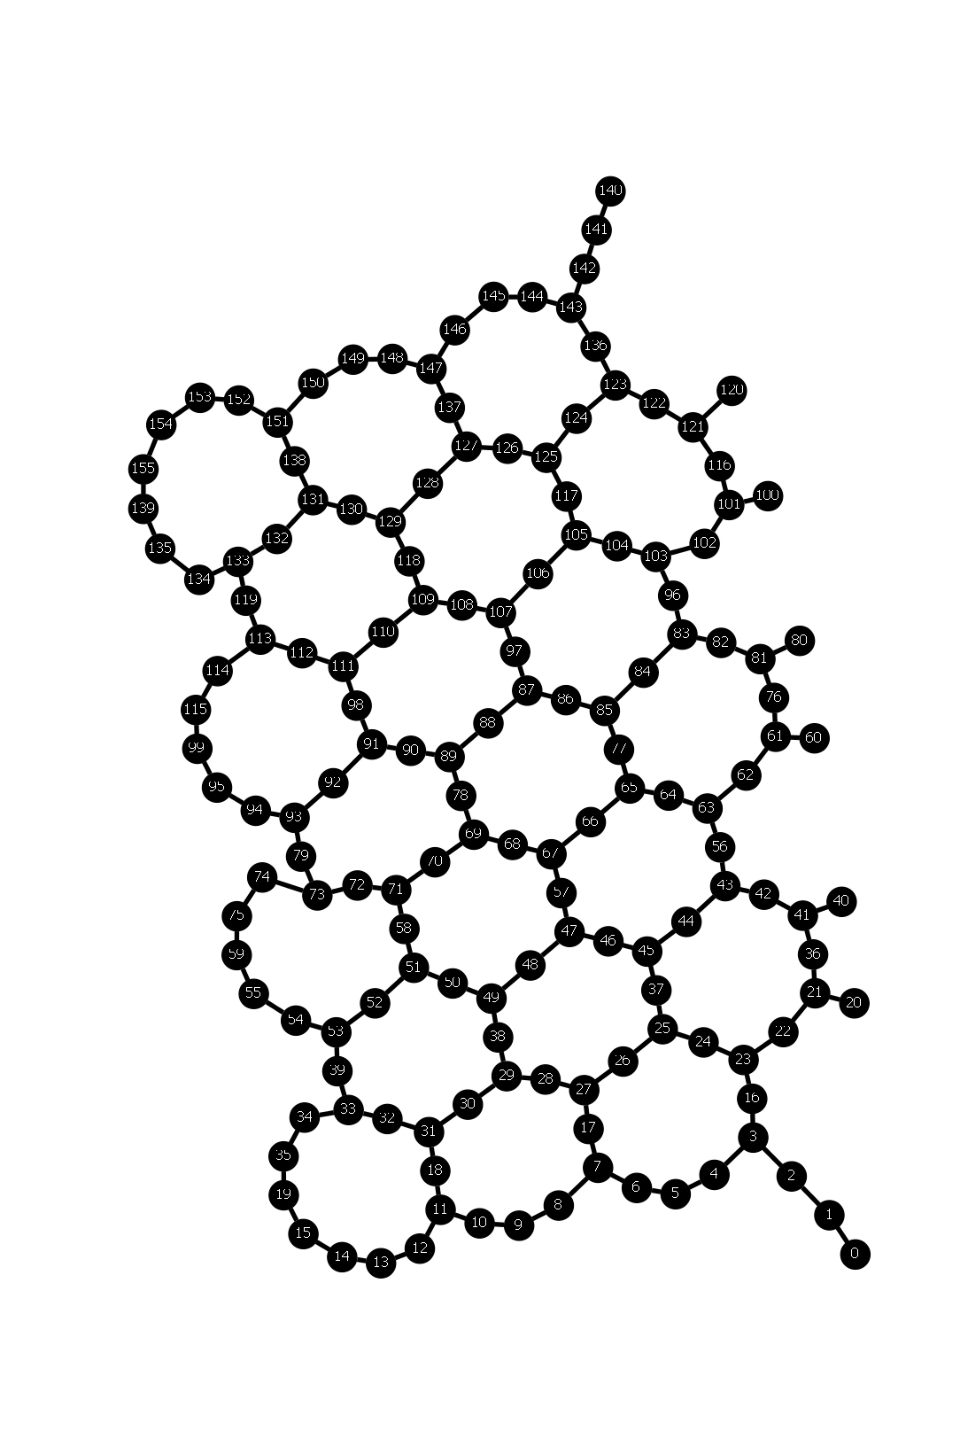
\includegraphics[width=\textwidth]{figure13.png}\\
\end{minipage} & 
\begin{minipage}{0.3\textwidth}
  \centering
  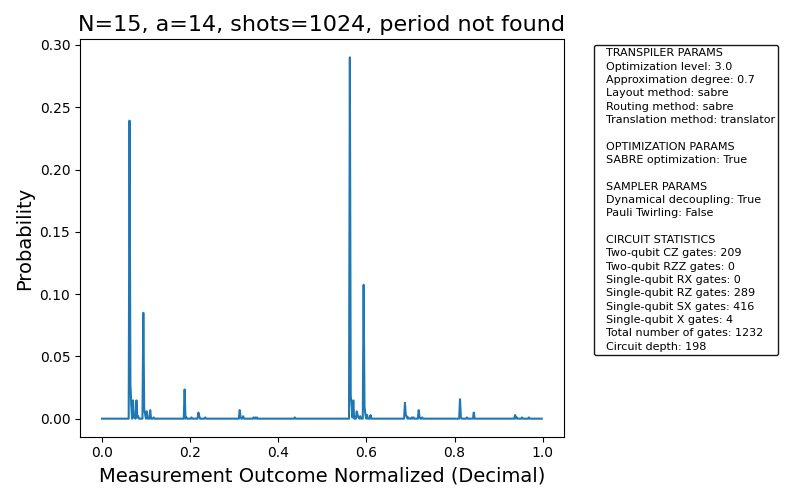
\includegraphics[width=\textwidth]{figure15.png}\\
\end{minipage} \\[1.5cm]

\begin{minipage}{0.1\textwidth}
  \centering
  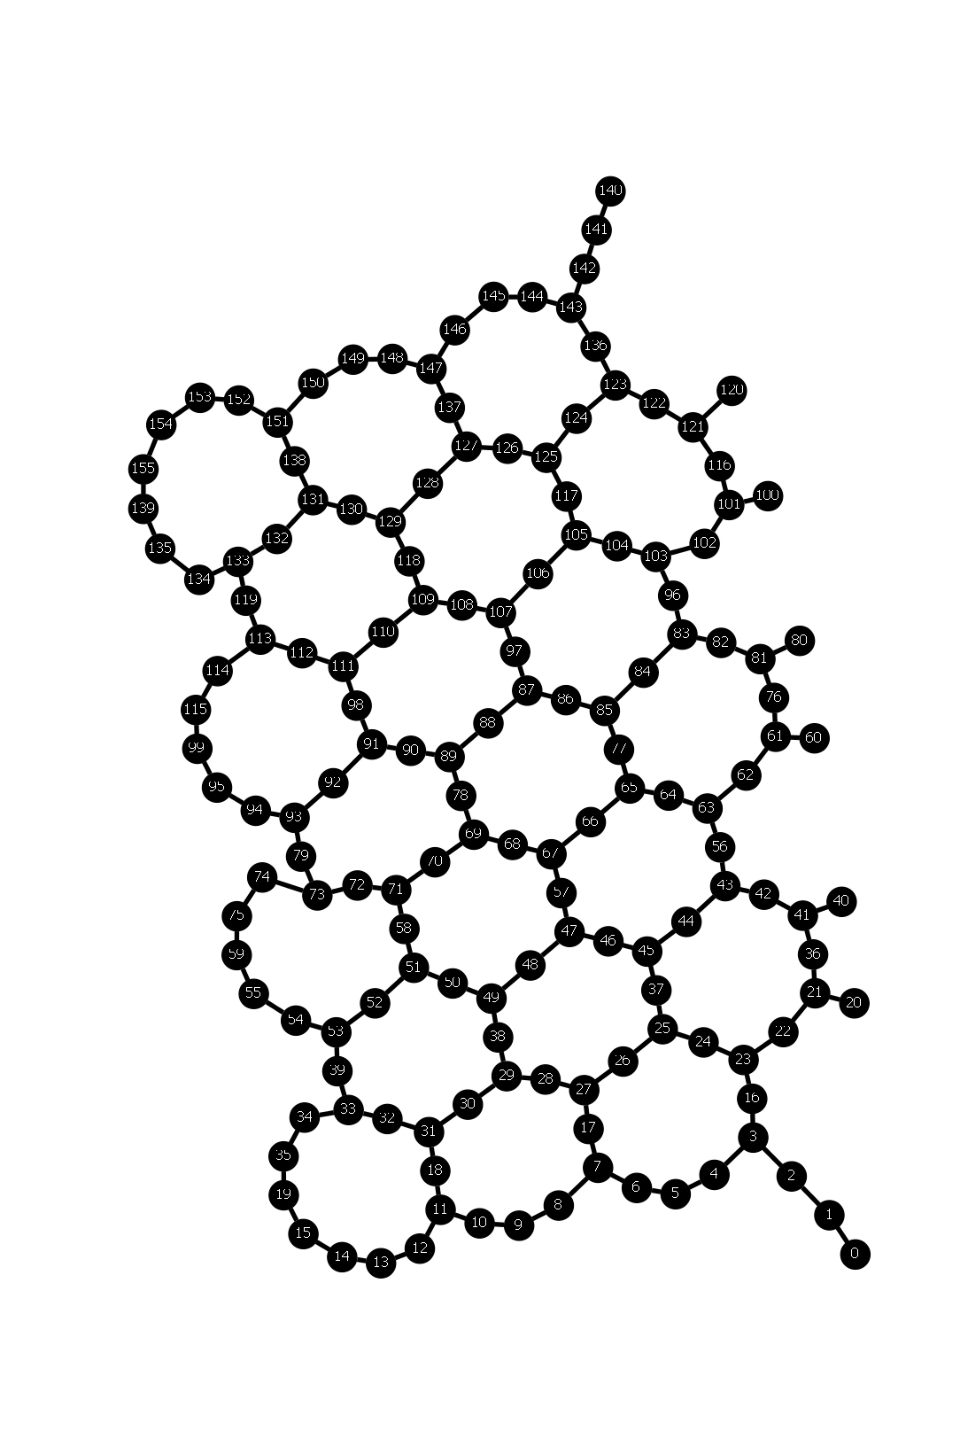
\includegraphics[width=\textwidth]{figure16b.png}\\
  \small (f)
\end{minipage} & 
\begin{minipage}{0.3\textwidth}
  \centering
  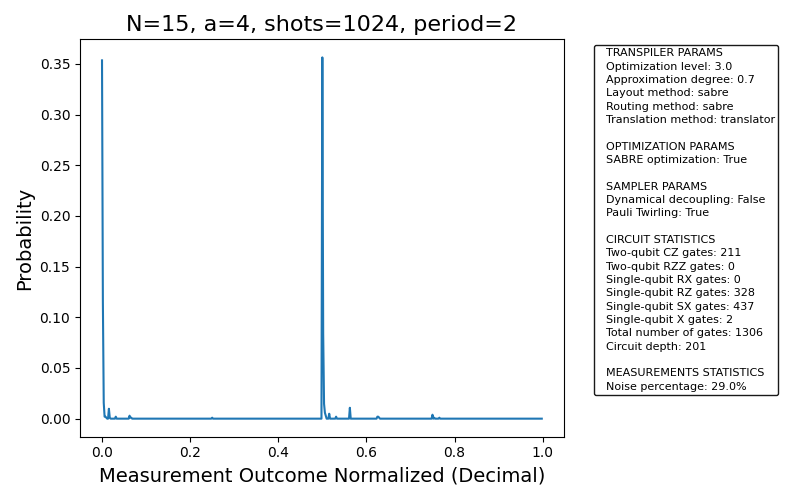
\includegraphics[width=\textwidth]{figure18b.png}\\
\end{minipage} & 
\begin{minipage}{0.1\textwidth}
  \centering
  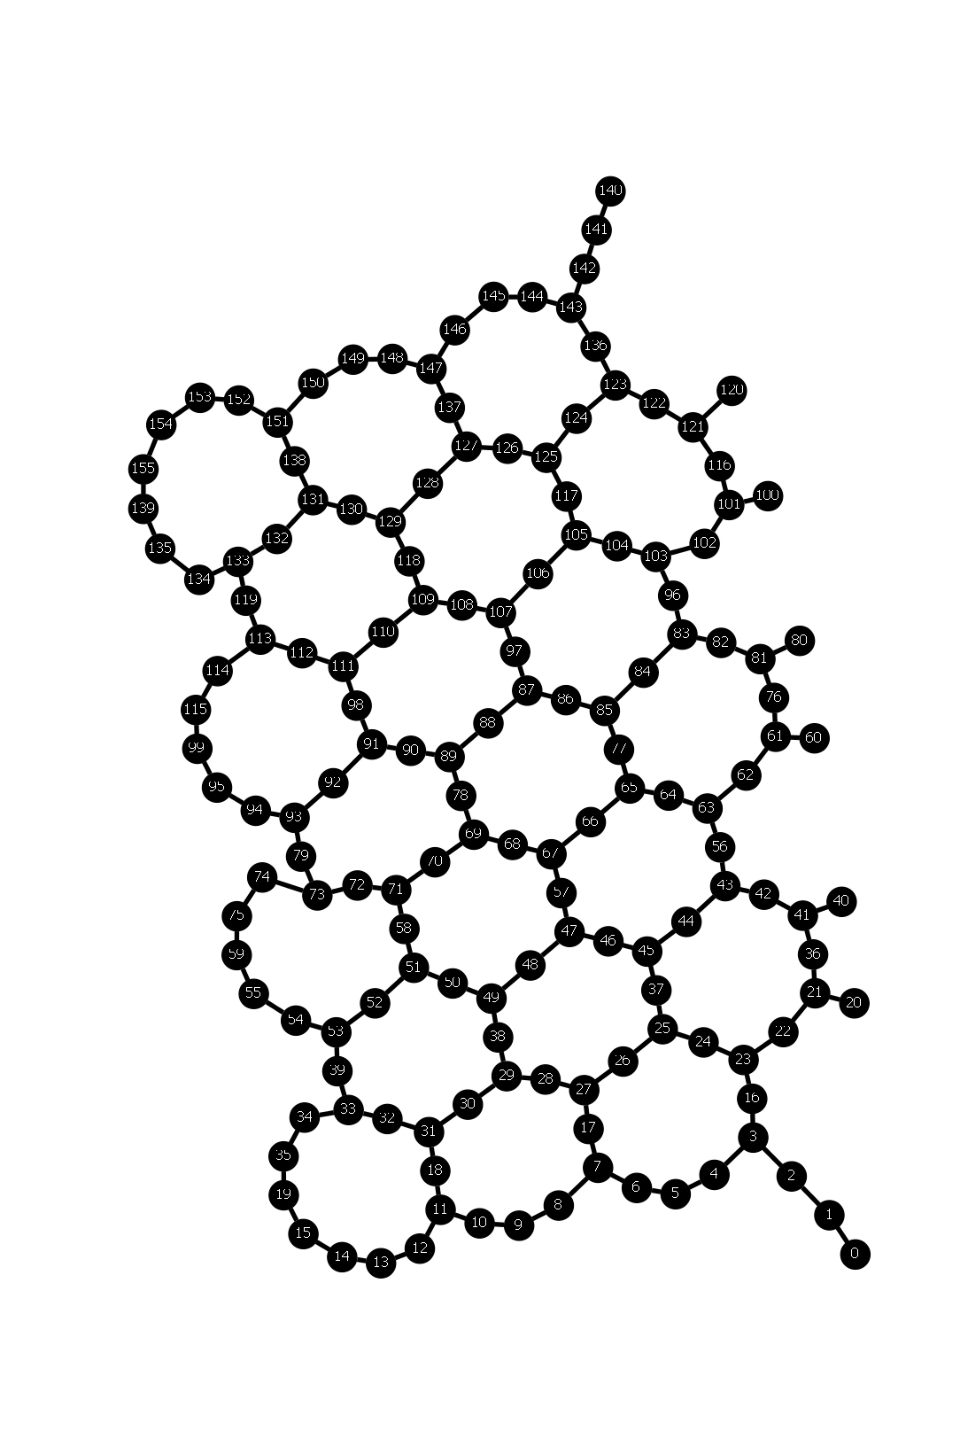
\includegraphics[width=\textwidth]{figure16.png}\\
\end{minipage} & 
\begin{minipage}{0.3\textwidth}
  \centering
  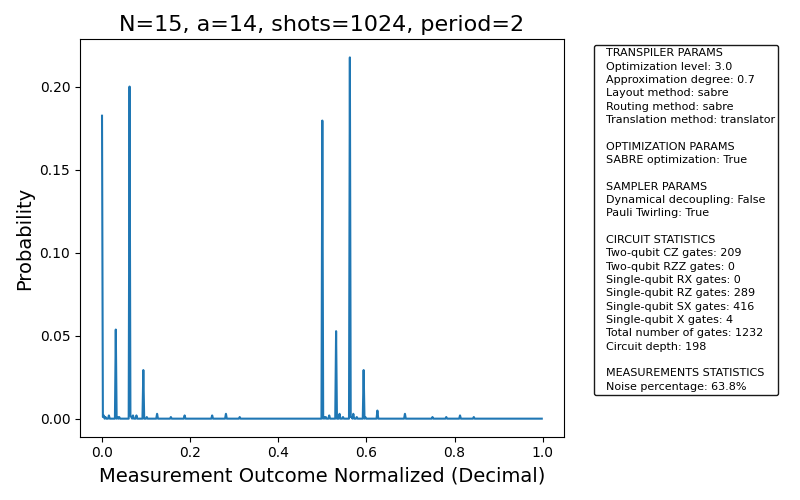
\includegraphics[width=\textwidth]{figure18.png}\\
\end{minipage} \\[1.5cm]

\begin{minipage}{0.1\textwidth}
  \centering
  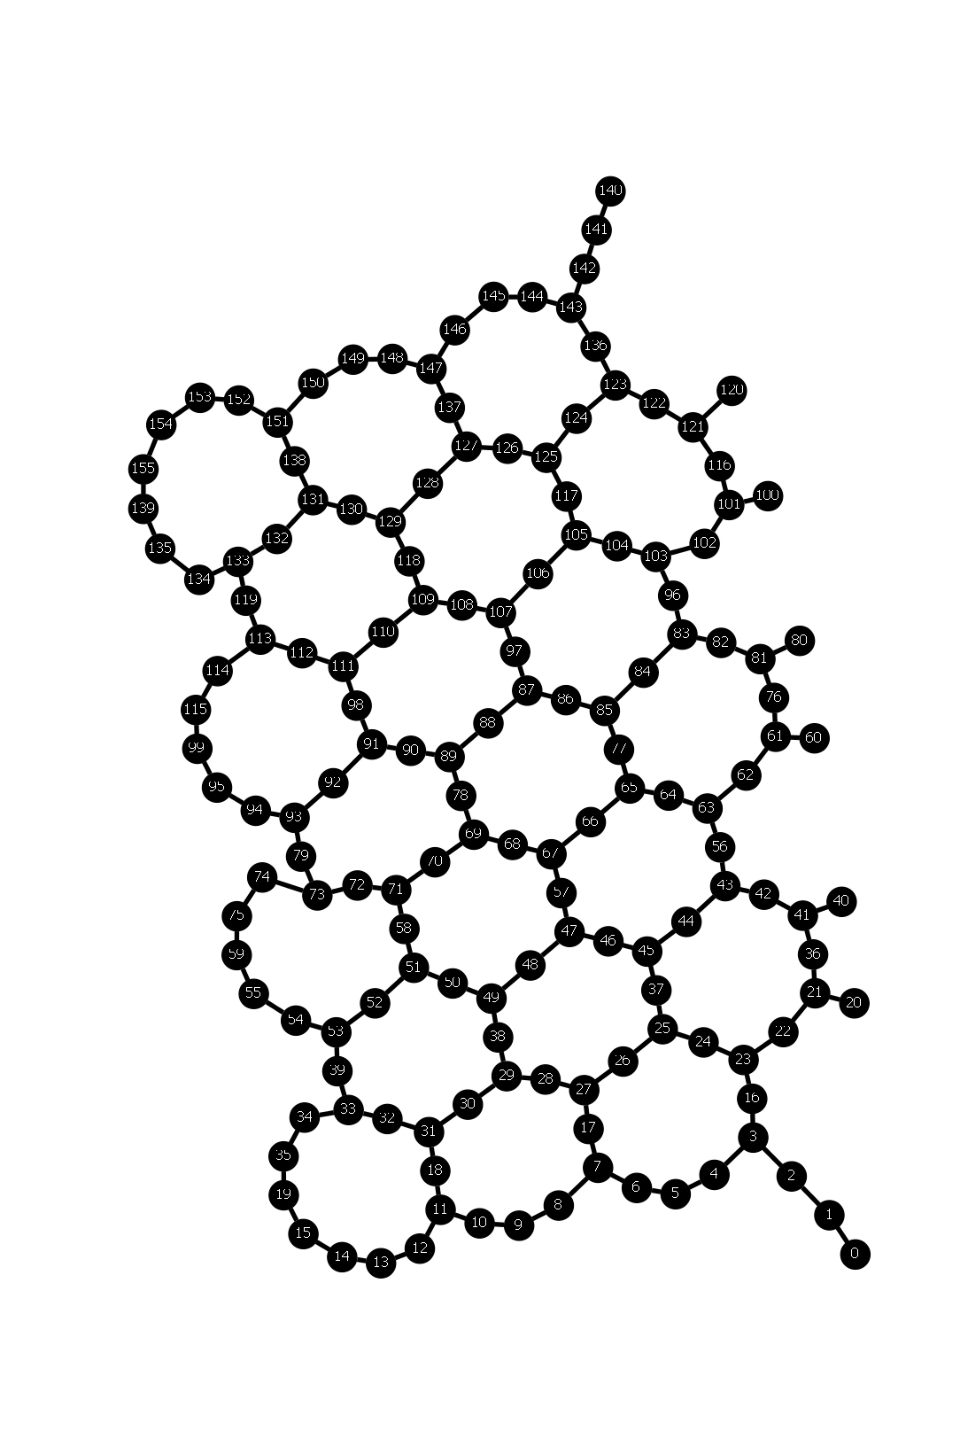
\includegraphics[width=\textwidth]{figure19b.png}\\
  \small (g)
\end{minipage} & 
\begin{minipage}{0.3\textwidth}
  \centering
  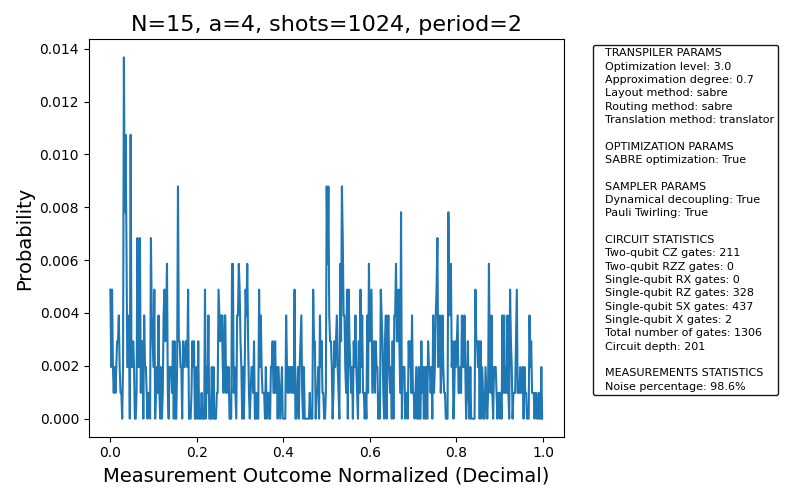
\includegraphics[width=\textwidth]{figure21b.png}\\
\end{minipage} & 
\begin{minipage}{0.1\textwidth}
  \centering
  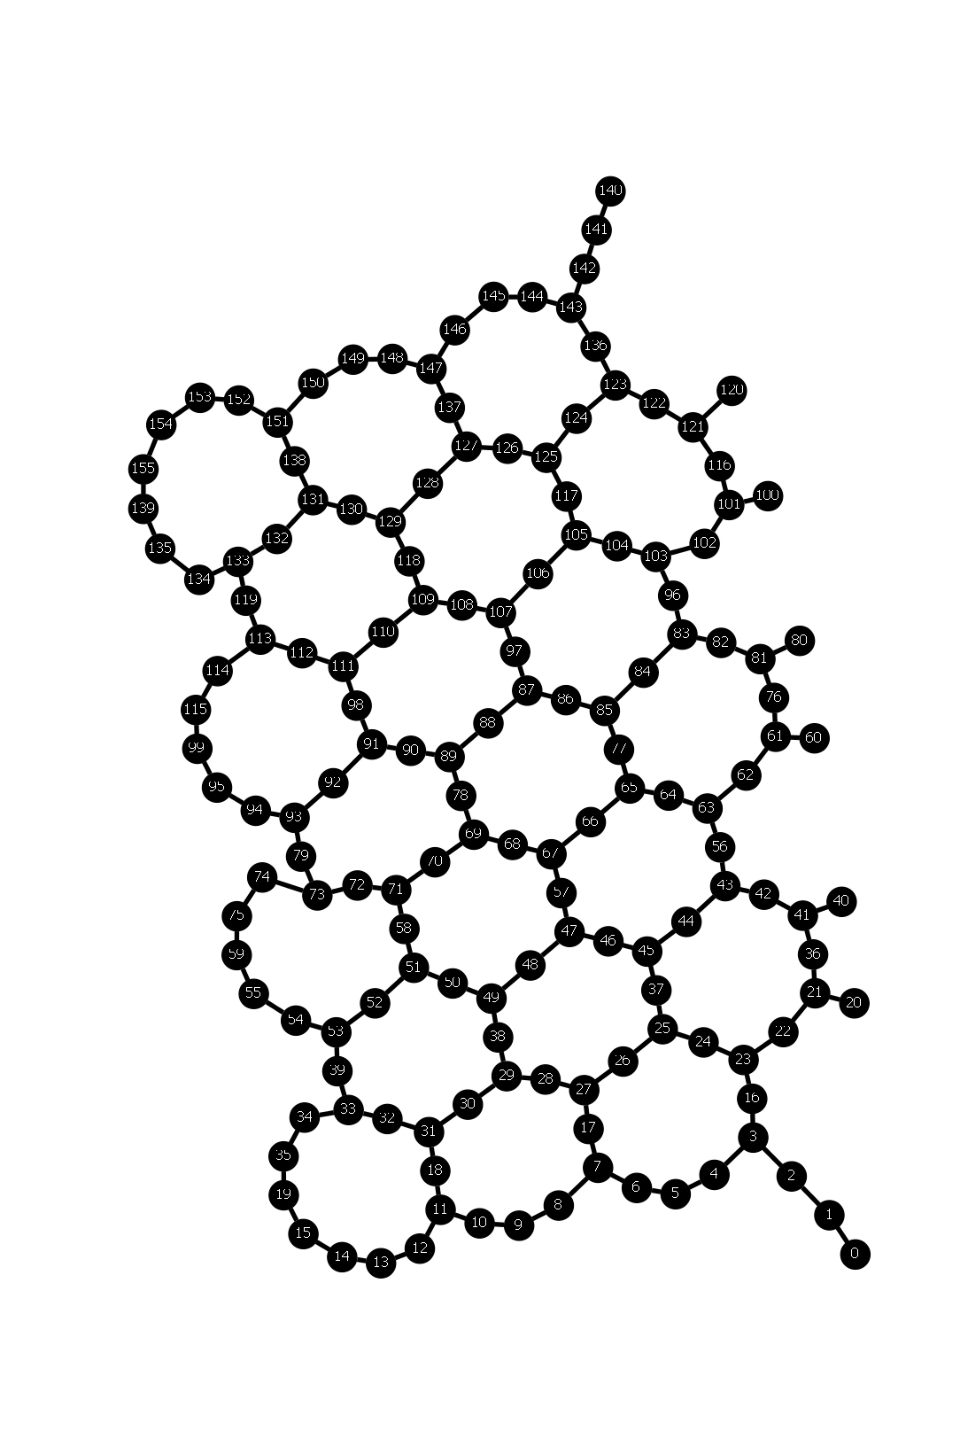
\includegraphics[width=\textwidth]{figure19.png}\\
\end{minipage} & 
\begin{minipage}{0.3\textwidth}
  \centering
  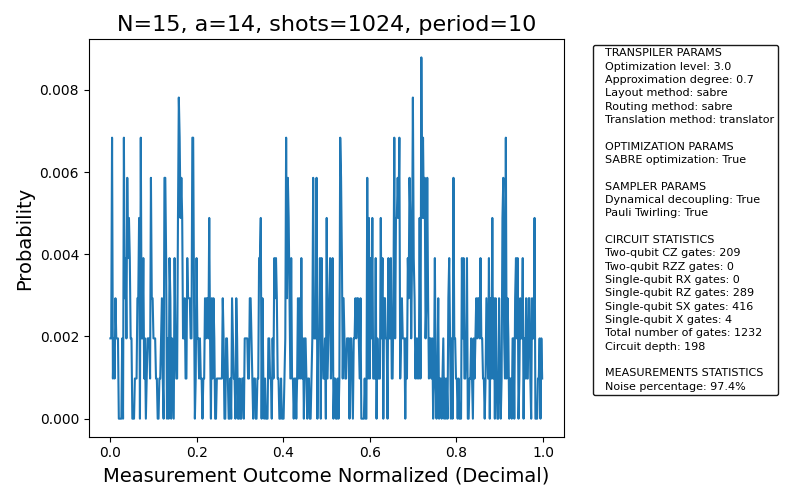
\includegraphics[width=\textwidth]{figure21.png}\\
\end{minipage} \\[1.5cm]

\bottomrule
\end{tabular*}
\caption{Summary Table of Optimization and Error Mitigation Results (see text for details)}
\label{tab:wide_table}
\end{figure*}

\\


\subsubsection{Exploring the maximum value of $N$ that can be factored - Part I }

In this section, we explore the maximum values of $N$ that can be factored, which are much larger than the academic case of $N=15$ used in previous sections to understand the influence of different parameters. At the time of writing this report, with optimization level = 0 and approximation degree = 1, we successfully factored up to $N=26$ transpiling and executing the circuits for all values of $a$ coprime of $N$, and finding the correct period $r$ for at least one value of $a$\footnote{Note: Shor's algorithm doesn't need to work for all values of $a$ - it only needs to work for a sufficient fraction of them to be practical. When factoring an integer $N$, a random value of $a$ coprime to $N$ has to be selected and we have to try to find the period of the function \(f(x) = a^x \ mod \ N\). The algorithm succeeds in factoring $N$ when this period $r$ is \textbf{even} and \(a^{r/2} ≢ ±1 (mod N) \), because then \(gcd(a^{r/2} ± 1, N) \) gives a non-trivial factor. The crucial theoretical result is that for any odd composite $N$ that is not a prime power, at least half of the values of $a$ coprime to $N$ will yield a period that leads to successful factoring. This means that there are at least a 50\% chance of success on each attempt. In practice, if one choice of a fails, another random $a$ is selected and the process is repeated. The expected number of attempts is at most 2, and with high probability it will succeed in a few tries.}.

The use of identical optimization parameters (optimization level 3, approximation factor 0.7, and Pauli Twirling) allows us to isolate the effects of problem size on quantum circuit complexity and performance. Using these parameters, we also successfully factored $N=51$, $N=55$, $N=57$, and $N=65$, by searching at least a value of $a$ among all the coprimes of $N$, for which the correct period $r$ is found, as suggested in Shor's algorithm. In the next sections a more efficient approach is presented that allows to factor even larger $N$'s.

 For $N=51$ all values of $a$ coprime of $N$ lead to feasible circuits. Results are shown in Table \ref{tab:QC_statistics_N=51_all_a}. We believe this is due to the fact that all values of $r$ are powers of 2. For larger values of $N$ the fraction of the total number of circuits that can be transpiled rapidly decreases. Results for for $N=55$, $N=57$, and $N=65$ are presented in Tables \ref{tab:QC_statistics_N=55_all_a}, \ref{tab:QC_statistics_N=57_all_a}, and \ref{tab:QC_statistics_N=65_all_a}. Figures \ref{tab:Factoring_N=55}, \ref{tab:Factoring_N=57}, and \ref{tab:Factoring_N=65} present the actual circuit layouts and their probability distributions, respectively. 

\begin{itemize}
    \item \textbf{Circuit Feasibility and Scaling}: The transition from $N=55$ to $N=65$ reveals significant scaling challenges in quantum factoring. For $N=55$, 7 out of 40 coprime values ($a = 12, 21, 23, 32, 34, 43, 54$) produced feasible circuits that could be transpiled and executed successfully, requiring between 14,819 and 81,641 total gates and circuit depths between 2,708 and 14,708. For $N=57$, only 3 out of 36 coprimes ($a = 20, 37, 56$) were feasible, with gate counts between 29,938 and 40,428 and depths between 5,723 and 7,494. For $N=65$, only 2 out of 47 coprimes ($a = 14, 51$) were feasible, with gate counts of 161,286 and 166,981, and circuit depths of 29,280 and 30,129, respectively. Non-feasible cases for $N>65$ required over 2 million gates, a $\sim$13--15$\times$ increase over feasible cases, highlighting a bimodal distribution and extreme dependence on the choice of $a$.

    \item \textbf{Gate Distribution Patterns}: For $N=55$, RZ and CZ gates dominated complexity, with no RX or RZZ gates. For $N=57$, SX gates were prominent alongside CZ gates. For $N=65$, a stark shift occurred: no RZ or SX gates were used, with CZ gates (e.g., 62348 for $a=14$, 64816 for $a=51$) and RX gates (e.g., 29627 for $a=14$, 30524 for $a=51$) dominating, indicating a change in circuit synthesis strategy or basis gate decomposition on the \texttt{ibm\_aachen} QPU.

    \item \textbf{Circuit Depth Analysis}: Circuit depths for $N=55$ ranged from 2,708 to 14,708 (average $\sim$11,600), while $N=57$ feasible cases had lower depths (5,723--7,494). For $N=65$, feasible cases had significantly higher depths (29,280 for $a=14$, 30,129 for $a=51$), reflecting increased circuit complexity despite fewer feasible cases, possibly due to larger modular exponentiation requirements.

    \item \textbf{Noise Performance Comparison}: Histogram noise levels for $N=55$ varied widely (10.3\%--55.2\%), while $N=57$ feasible cases showed better consistency (13.7\%--19.3\%). For $N=65$, noise levels were higher (56.3\% for $a=14$, 55.3\% for $a=51$), suggesting that larger $N$ values increase susceptibility to decoherence and gate errors, even in feasible cases, likely due to deeper circuits.

    \item \textbf{Success Rate}: Success rates decreased with increasing $N$: 17.5\% (7/40) for $N=55$, 8.3\% (3/36) for $N=57$, and only 4.3\% (2/47) for $N=65$. The consistent $r=2$ period finding in successful $N=57$ and $N=65$ cases, compared to mixed $r=2$ and $r=4$ for $N=55$, suggests that shorter periods produce more favorable quantum interference patterns, which will be used later to optimize the overall algorithm, although the reduced number of feasible $a$ values for $N=65$ indicates tighter constraints. 
\end{itemize}

These results highlight the exponential scaling challenges in near-term quantum factoring. The drastic reduction in feasible cases from $N=55$ to $N=57$ and $N=65$ confirms current hardware limitations, with $N=65$ pushing the boundaries of what is achievable running Shor's algorithm\footnote{Recall that the largest value of $N$ that has been factorized in an IBM NISQ is $N=21$ \citep*{Karamlou2021}. }. The sensitivity to $a$ could be leveraged by developing classical pre-processing to identify tractable cases before transpilation, as explored in later sections. This fact and further tunning of the circuit optimizations will show how to beat this record much further.

\begin{table}[h]
\centering
\caption{Quantum Circuit Statistics for $N=51$ and all $a$ Coefficients, transpiled and successfully executed in an \texttt{ibm\_aachen} QPU with Optimization Degree = 3, Approximation Factor = 0.7, and Pauli Twirling. Number of RX, RZ, SX, X, CZ, and RZZ gates not shown for the sake of simplificy.}
\label{tab:QC_statistics_N=51_all_a}
\begin{tabular}{c c c c c}
\toprule
\textbf{$a$} & \textbf{$r$} & \textbf{Total Gates} & \textbf{Circuit Depth} & \textbf{Histogram Noise (\%)} \\
\midrule
2 & 4 & 120545 & 21999 & 56.0\% \\
4 & 4 & 7993 & 14377 & 54.1\% \\
5 & 16 & 159739 & 28752 & 54.0\% \\
7 & 16 & 167981 & 30384 & 10.4\% \\
8 & 8 & 125261 & 22862 & 12.3\% \\
10 & 16 & 165820 & 29740 & 50.8\% \\
11 & 16 & 162097 & 29364 & 8.5\% \\
13 & 4 & 83114 & 15222 & 55.7\% \\
14 & 16 & 165516 & 30046 & 17.4\% \\
16 & 2 & 40912 & 22464 & 15.6\% \\
20 & 8 & 124846 & 22762 & 20.5\% \\
22 & 16 & 168841 & 30405 & 11.0\% \\
23 & 16 & 165424 & 30063 & 6.8\% \\
25 & 8 & 121014 & 21991 & 53.1\% \\
26 & 8 & 120188 & 21737 & 13.8\% \\
28 & 16 & 168554 & 30523 & 12.3\% \\
29 & 16 & 163706 & 29340 & 7.9\% \\
31 & 16 & 167359 & 30516 & 15.3\% \\
32 & 8 & 119874 & 21498 & 17.3\% \\
35 & 2 & 36800 & 6641 & 19.8\% \\
37 & 16 & 163522 & 29621 & 8.6\% \\
38 & 4 & 78433 & 14041 & 13.8\% \\
40 & 16 & 164321 & 29704 & 15.9\% \\
41 & 16 & 159830 & 28623 & 13.7\% \\
43 & 8 & 124186 & 22325 & 9.8\% \\
44 & 16 & 169469 & 30758 & 16.0\% \\
46 & 16 & 162817 & 29426 & 5.0\% \\
47 & 4 & 81351 & 14835 & 16.0\% \\
49 & 8 & 122173 & 21871 & 9.4\% \\
50 & 2 & 22227 & 4001 & 22.4\% \\
\bottomrule
\end{tabular}
\end{table}


\begin{table*}[h]
\centering
\caption{Quantum Circuit Statistics for $N=55$ and Different $a$ Coefficients, transpiled and successfully executed in an \texttt{ibm\_aachen} QPU with Optimization Degree = 3, Approximation Factor = 0.7, and Pauli Twirling}
\label{tab:QC_statistics_N=55_all_a}
\begin{tabular}{rrrrrrrrrrr}
\toprule
$a$ & r & RX Gates & RZ Gates & SX Gates & X Gates & CZ Gates & RZZ Gates & Total Gates & Circuit Depth & Histogram Noise\\
\midrule
2 & 20 & 0  & 157208 & 207123 & 1520  & 99718  & 0  & 540867 & 97577 & -- \\
3 & 20 & 0  & 128448 & 168759 & 1241  & 82130  & 0  & 443273 & 80240 & --   \\
4 & 10 & 0  & 157776 & 207743 & 1470  & 99736  & 0  & 541719 & 97416 & --   \\
6 & 10 & 0  & 160202 & 210171 & 1365  & 100747 & 0  & 548277 & 98428 & --   \\
7 & 20 & 0  & 157059 & 205616 & 1432  & 98474  & 0  & 536858 & 96030 & --   \\
8 & 20 & 0  & 160987 & 211291 & 1505  & 101461 & 0  & 551608 & 99152 & --   \\
9 & 10 & 0  & 160953 & 209666 & 1505  & 100006 & 0  & 547208 & 97585 & --   \\
12 & 4 & 0  & 22424  & 29764  & 220   & 14317  & 0  & 77707  & 13983 & 55.2 \%   \\
13 & 20 & 0  & 160229 & 210390 & 1473  & 101030 & 0  & 549068 & 98727 & --   \\
14 & 10 & 0  & 158188 & 208378 & 1448  & 100295 & 0  & 543846 & 97913 & --   \\
16 & 5 & 0  & 158489 & 209443 & 1436  & 100980 & 0  & 546469 & 98659 & --   \\
17 & 20 & 0  & 157520 & 207896 & 1534  & 100343 & 0  & 543092 & 98110 & --   \\
18 & 20 & 0  & 161023 & 211001 & 1547  & 101239 & 0  & 550867 & 98830 & --   \\
19 & 10 & 0  & 161848 & 212553 & 1484  & 102212 & 0  & 554871 & 99942 & --   \\
\textbf{21} & \textbf{2} & \textbf{0} & \textbf{11768} & \textbf{15836}  & \textbf{95} & \textbf{7710}   & \textbf{0}  & \textbf{41350}  & \textbf{7548}  & \textbf{11.5 \%}   \\
23 & 4 & 0  & 23708  & 31171  & 216   & 15029  & 0  & 81641  & 14708 & 10.3 \%   \\
24 & 10 & 0  & 159993 & 210273 & 1403  & 100882 & 0  & 548393 & 98516 & --   \\
26 & 5 & 0  & 161906 & 211698 & 1444  & 101325 & 0  & 552441 & 98839 & --   \\
27 & 20 & 0  & 157804 & 207533 & 1484  & 99893  & 0  & 542094 & 97536 & --   \\
28 & 20 & 0  & 163940 & 214697 & 1360  & 102870 & 0  & 559992 & 100490& --   \\
29 & 10 & 0  & 161899 & 212874 & 1442  & 102197 & 0  & 555055 & 99831 & --   \\
31 & 5 & 0  & 161352 & 210506 & 1560  & 100813 & 0  & 549877 & 98352 & --   \\
32 & 4 & 0  & 23998  & 31624  & 225   & 15157  & 0  & 82603  & 14827 & 11.5 \%   \\
\textbf{34} & \textbf{2} & \textbf{0}  & \textbf{10919}  & \textbf{14591}  & \textbf{139}   & \textbf{7086}   & \textbf{0}  & \textbf{38299}  & \textbf{6943}  & \textbf{17.4 \%}   \\
36 & 5 & 0  & 160071 & 211031 & 1521  & 101569 & 0  & 550640 & 99207 & --   \\
37 & 20 & 0  & 158598 & 207544 & 1456  & 99212  & 0  & 541350 & 96694 & --   \\
38 & 20 & 0  & 159748 & 210176 & 1505  & 101262 & 0  & 548950 & 98929 & --   \\
39 & 10 & 0  & 158917 & 207965 & 1533  & 99688  & 0  & 543025 & 97373 & --   \\
41 & 10 & 0  & 158216 & 209086 & 1391  & 100759 & 0  & 545424 & 98472 & --   \\
42 & 20 & 0  & 158271 & 207320 & 1432  & 99373  & 0  & 541137 & 96949 & --   \\
43 & 4 & 0  & 23479  & 31035  & 213   & 14947  & 0  & 81098  & 14658 & 55.0 \%   \\
46 & 10 & 0  & 162943 & 214242 & 1395  & 102824 & 0  & 558556 & 100490& --   \\
47 & 20 & 0  & 161462 & 212062 & 1455  & 101386 & 0  & 552435 & 98950 & --   \\
48 & 20 & 0  & 159982 & 210329 & 1403  & 100979 & 0  & 548605 & 98605 & --   \\
49 & 10 & 0  & 163255 & 213794 & 1479  & 102408 & 0  & 557557 & 99896 & --   \\
51 & 10 & 0  & 165191 & 215721 & 1427  & 103214 & 0  & 562688 & 100643& --   \\
52 & 20 & 0  & 158870 & 209726 & 1443  & 100878 & 0  & 546876 & 98600 & --   \\
53 & 20 & 0  & 163249 & 213981 & 1459  & 102752 & 0  & 558234 & 100354& --   \\
\textbf{54} & \textbf{2} & \textbf{0}  & \textbf{4170}   & \textbf{5612}   & \textbf{31}    & \textbf{2793}   & \textbf{0}  & \textbf{14819}  & \textbf{2708}  & \textbf{17.3 \%}   \\
\bottomrule
\end{tabular}
\end{table*}

\begin{figure}[!htbp]
\centering
\begin{tabular}{p{0.45\textwidth}}
\toprule
\begin{minipage}{0.15\textwidth}
  \centering
  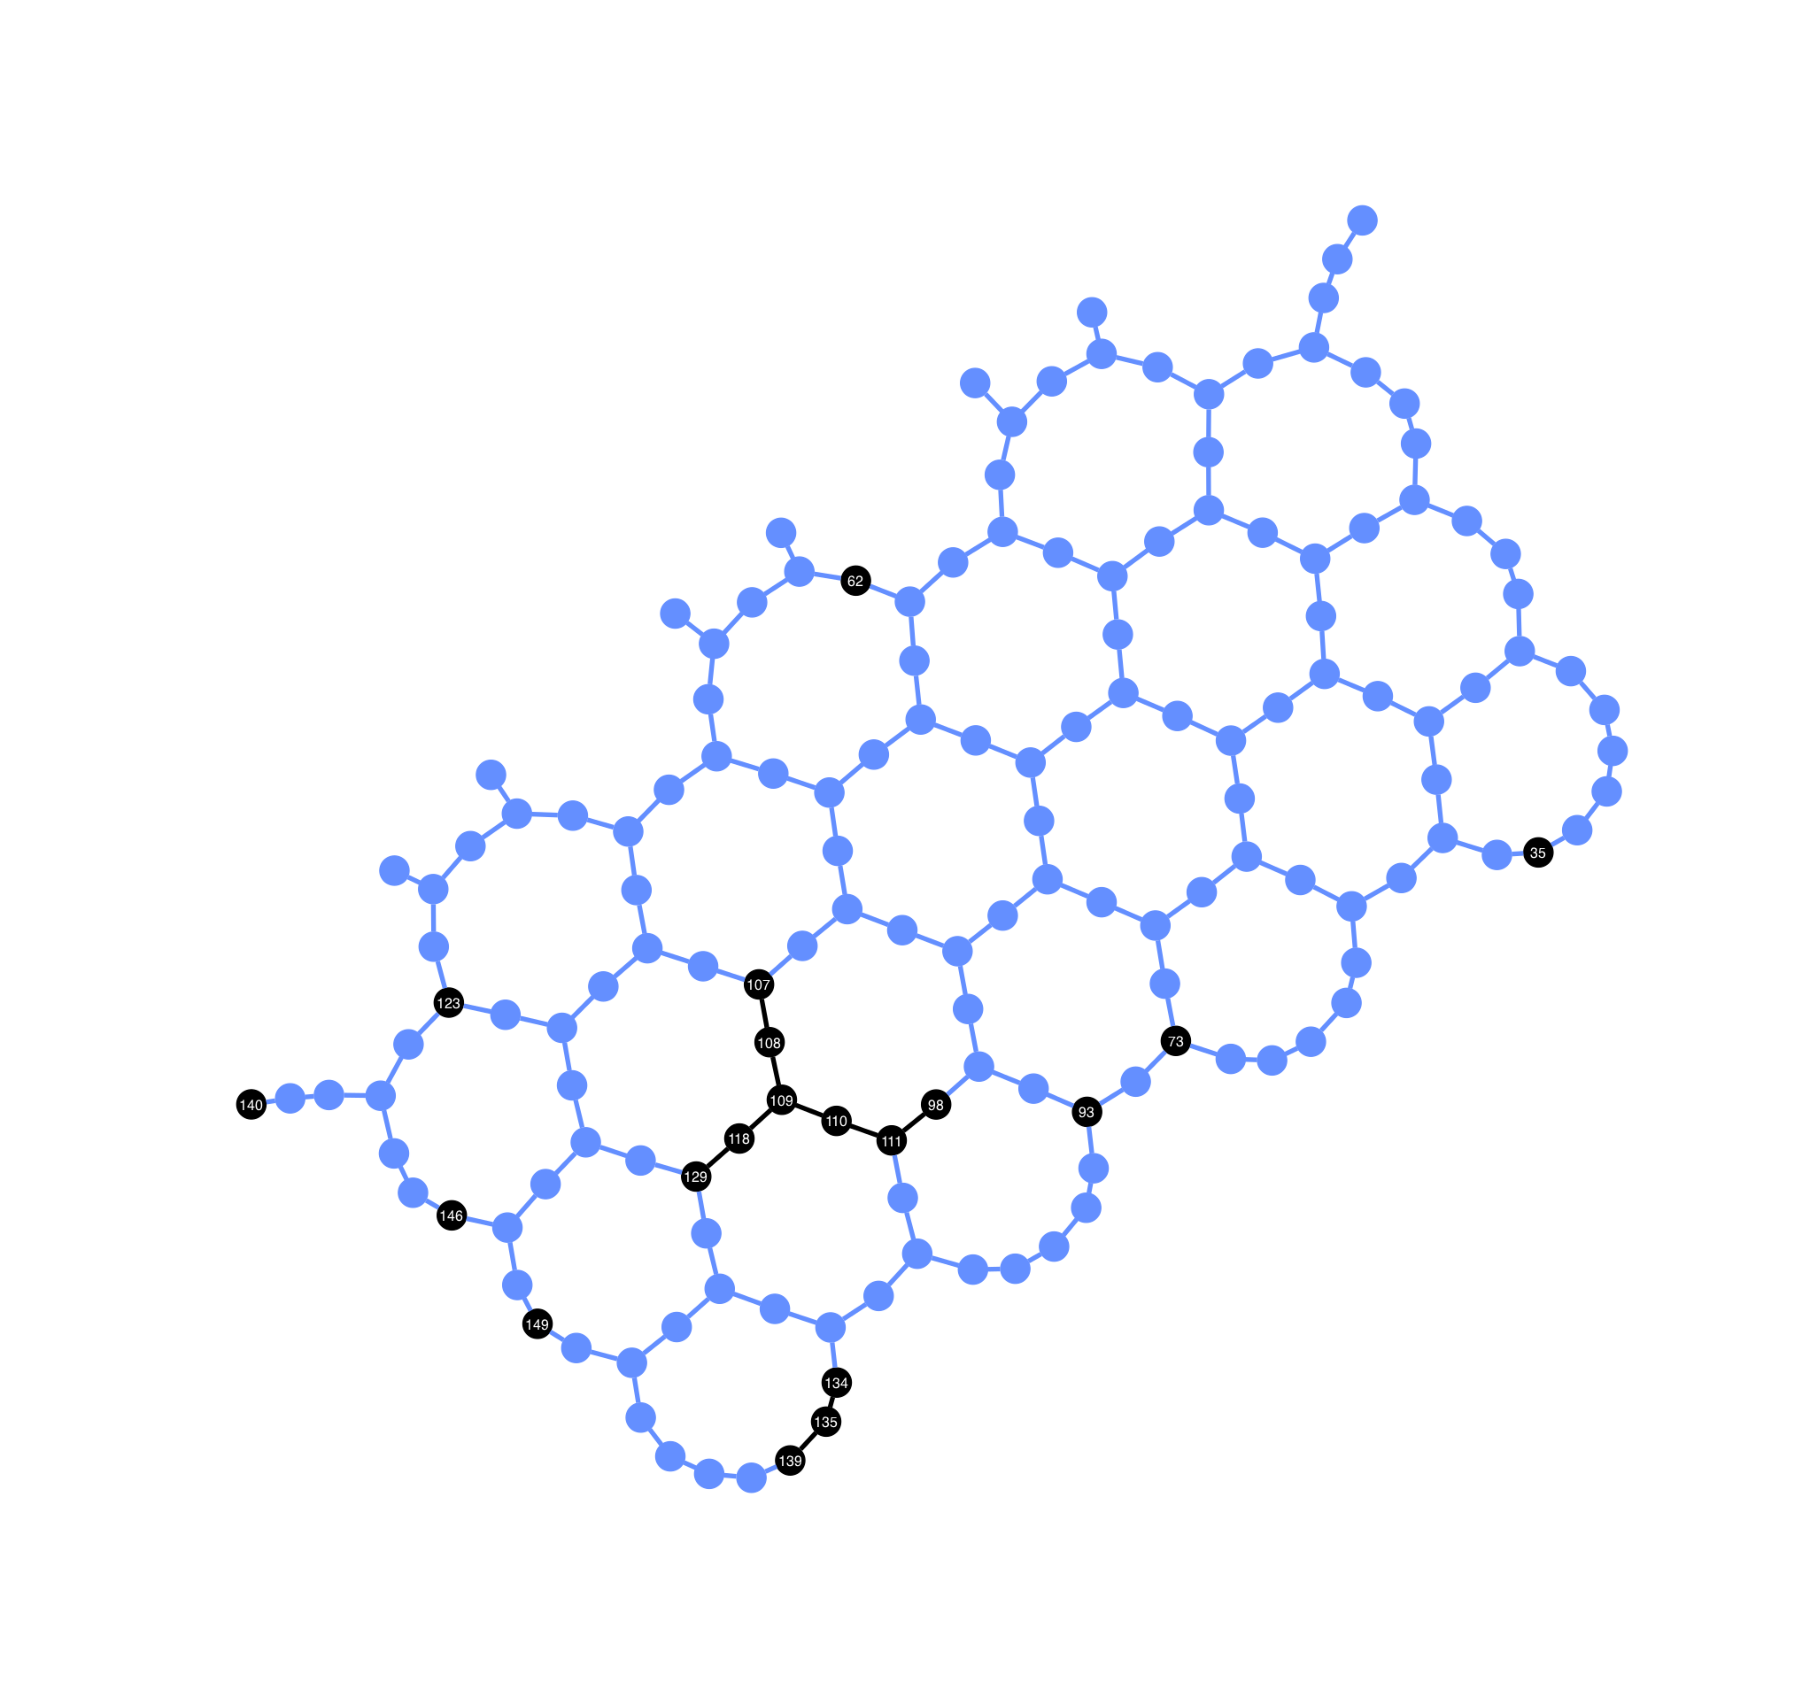
\includegraphics[width=\textwidth]{ibm_aachen_physical_circuit_layout_N55_a12.png} \\
  \small (a) $N=55$, $a=12$
\end{minipage} 
\begin{minipage}{0.3\textwidth}
  \centering
  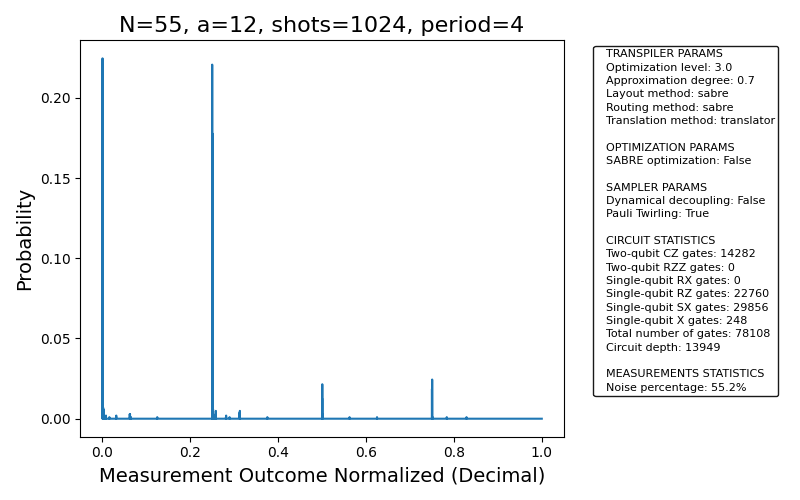
\includegraphics[width=\textwidth]{prob_dist_N55_a12_backend_ibmqpu.png} \\
\end{minipage} \\
\begin{minipage}{0.15\textwidth}
  \centering
  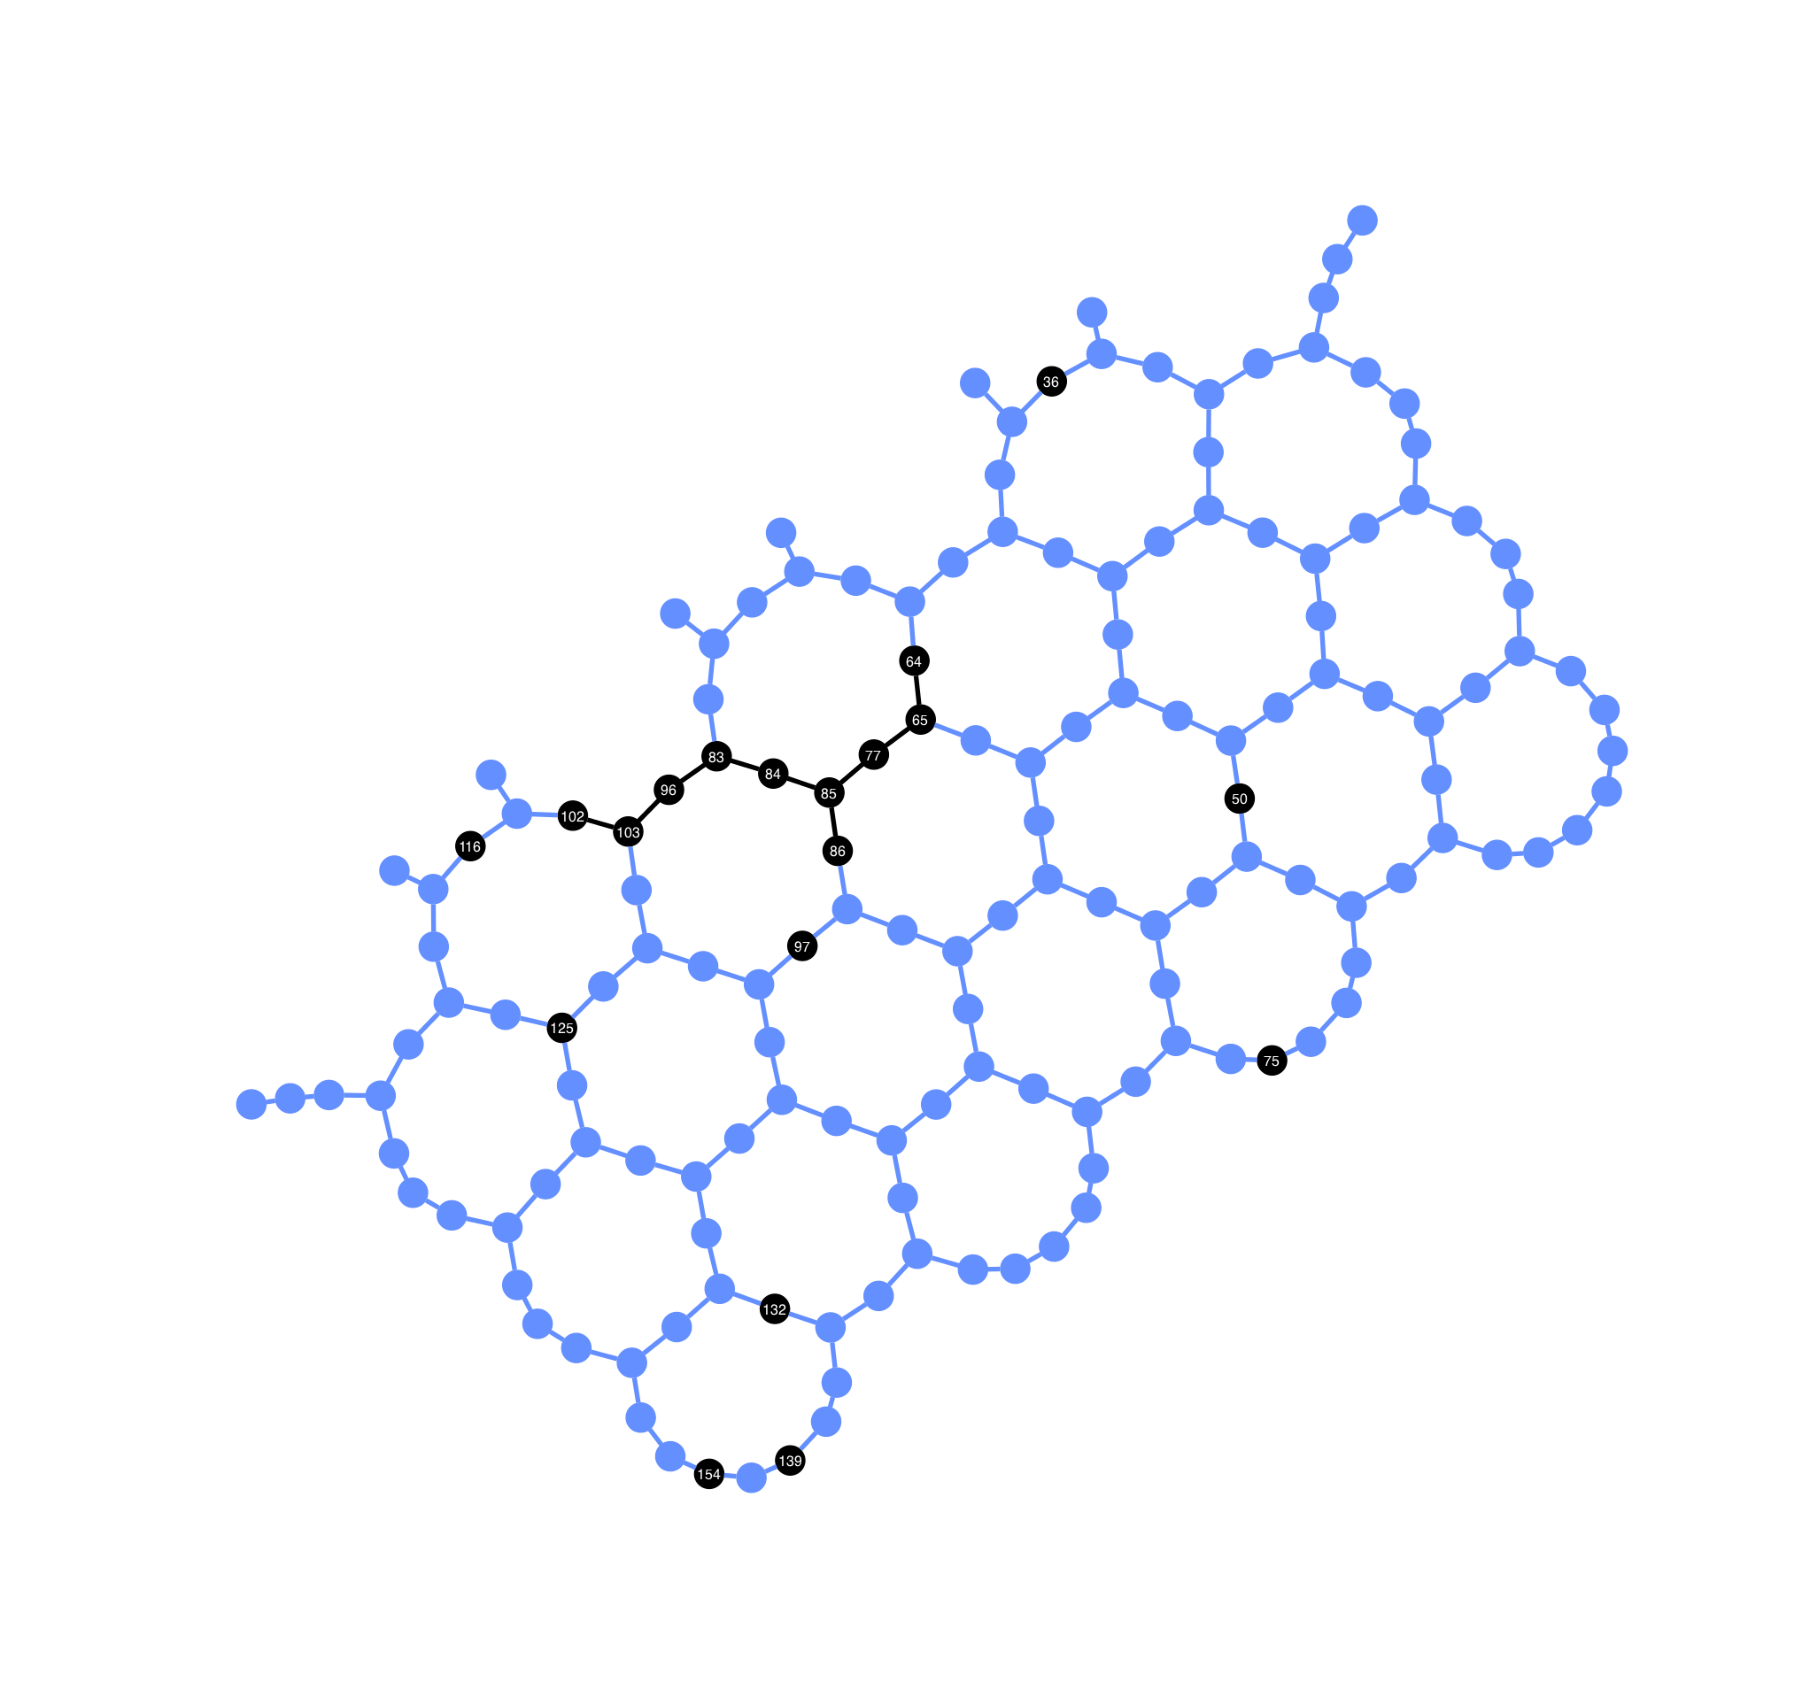
\includegraphics[width=\textwidth]{ibm_aachen_physical_circuit_layout_N55_a21.png} \\
  \small (a) $N=55$, $a=21$
\end{minipage} 
\begin{minipage}{0.3\textwidth}
  \centering
  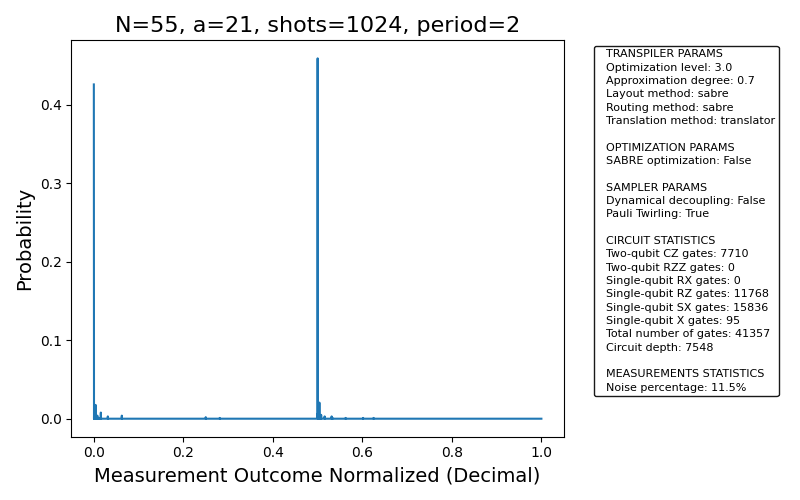
\includegraphics[width=\textwidth]{prob_dist_N55_a21_backend_ibmqpu.png} \\
\end{minipage} \\
\begin{minipage}{0.15\textwidth}
  \centering
  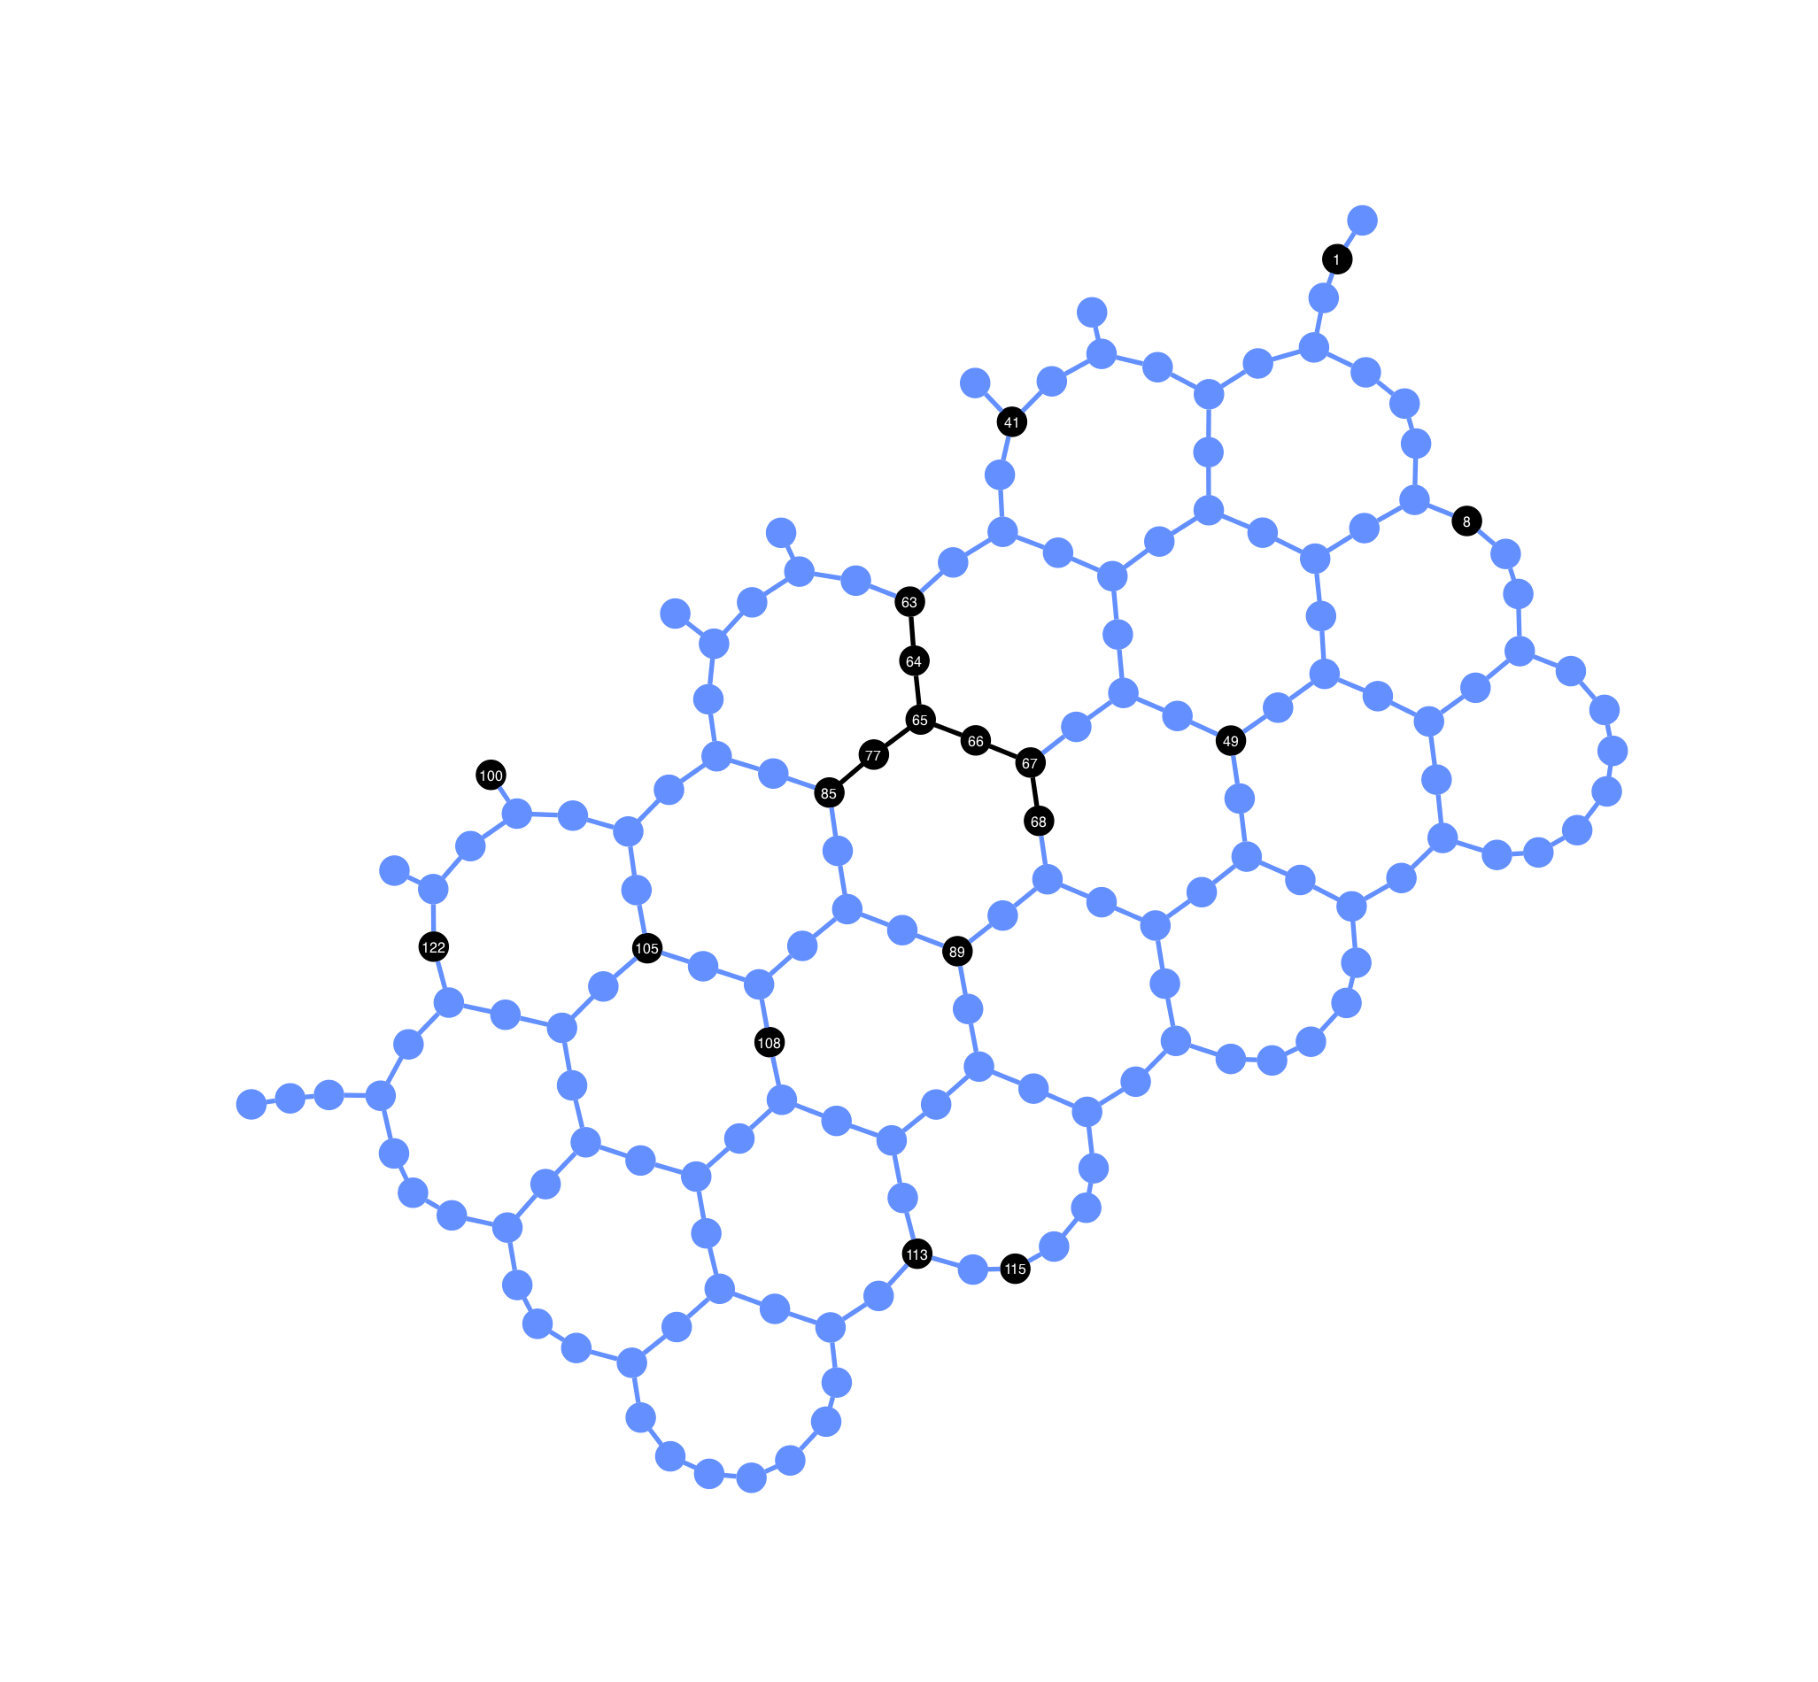
\includegraphics[width=\textwidth]{ibm_aachen_physical_circuit_layout_N55_a23.png} \\
  \small (a) $N=55$, $a=23$
\end{minipage} 
\begin{minipage}{0.3\textwidth}
  \centering
  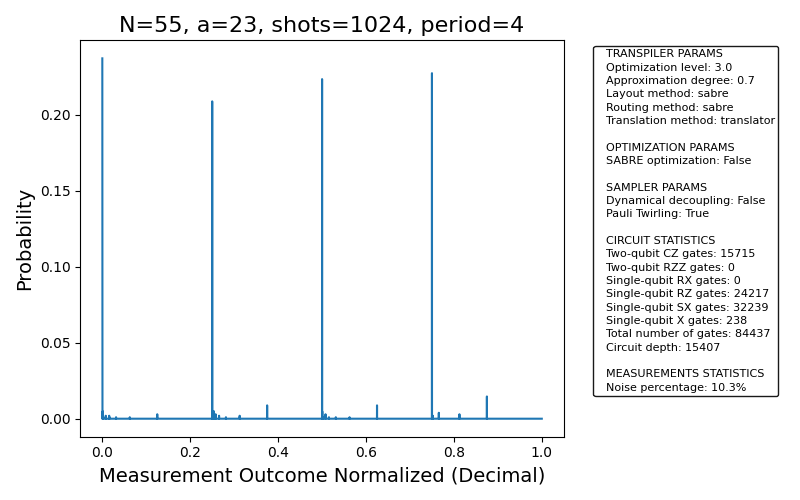
\includegraphics[width=\textwidth]{prob_dist_N55_a23_backend_ibmqpu.png} \\
\end{minipage} \\
\begin{minipage}{0.15\textwidth}
  \centering
  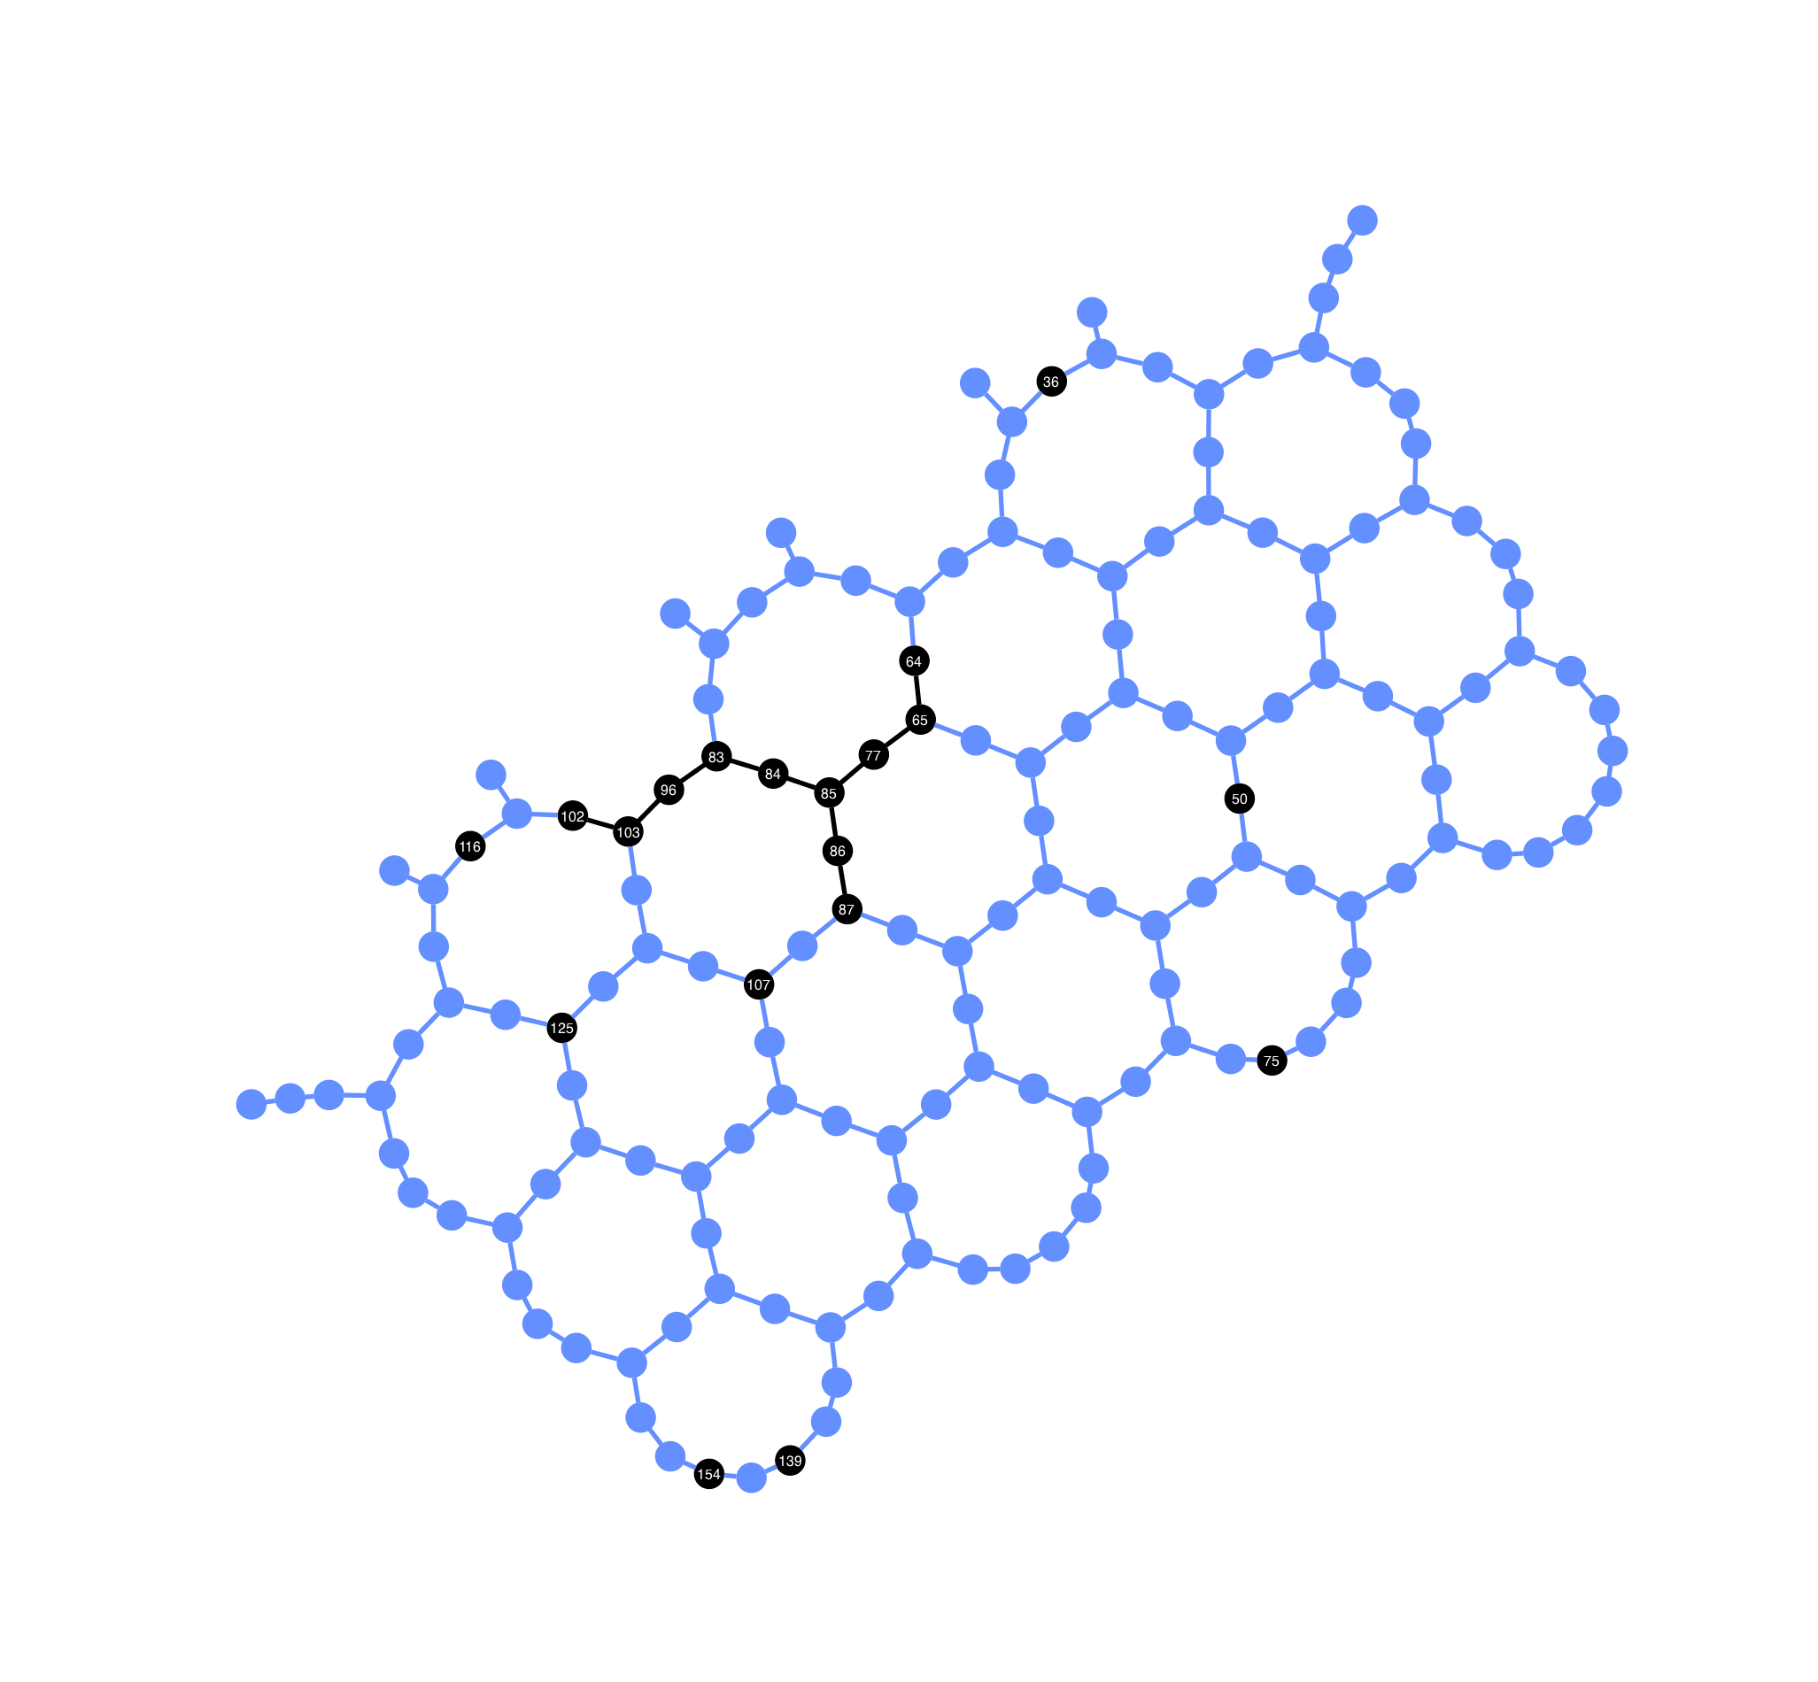
\includegraphics[width=\textwidth]{ibm_aachen_physical_circuit_layout_N55_a32.png} \\
  \small (a) $N=55$, $a=32$
\end{minipage} 
\begin{minipage}{0.3\textwidth}
  \centering
  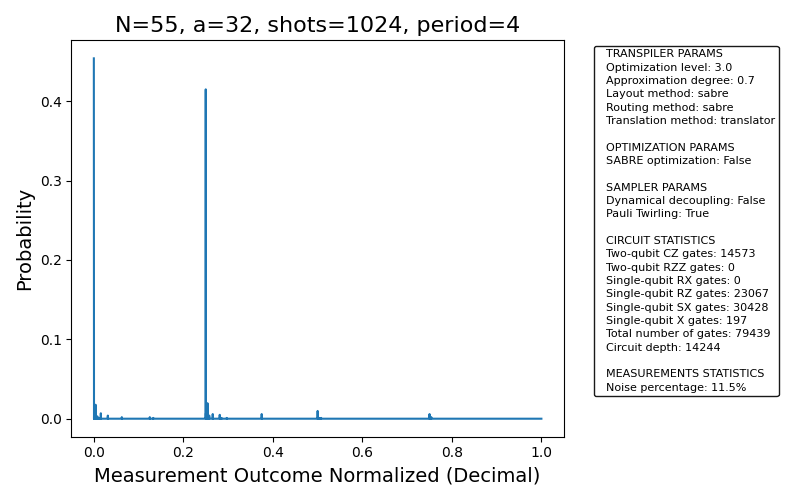
\includegraphics[width=\textwidth]{prob_dist_N55_a32_backend_ibmqpu.png} \\
\end{minipage} \\
\begin{minipage}{0.15\textwidth}
  \centering
  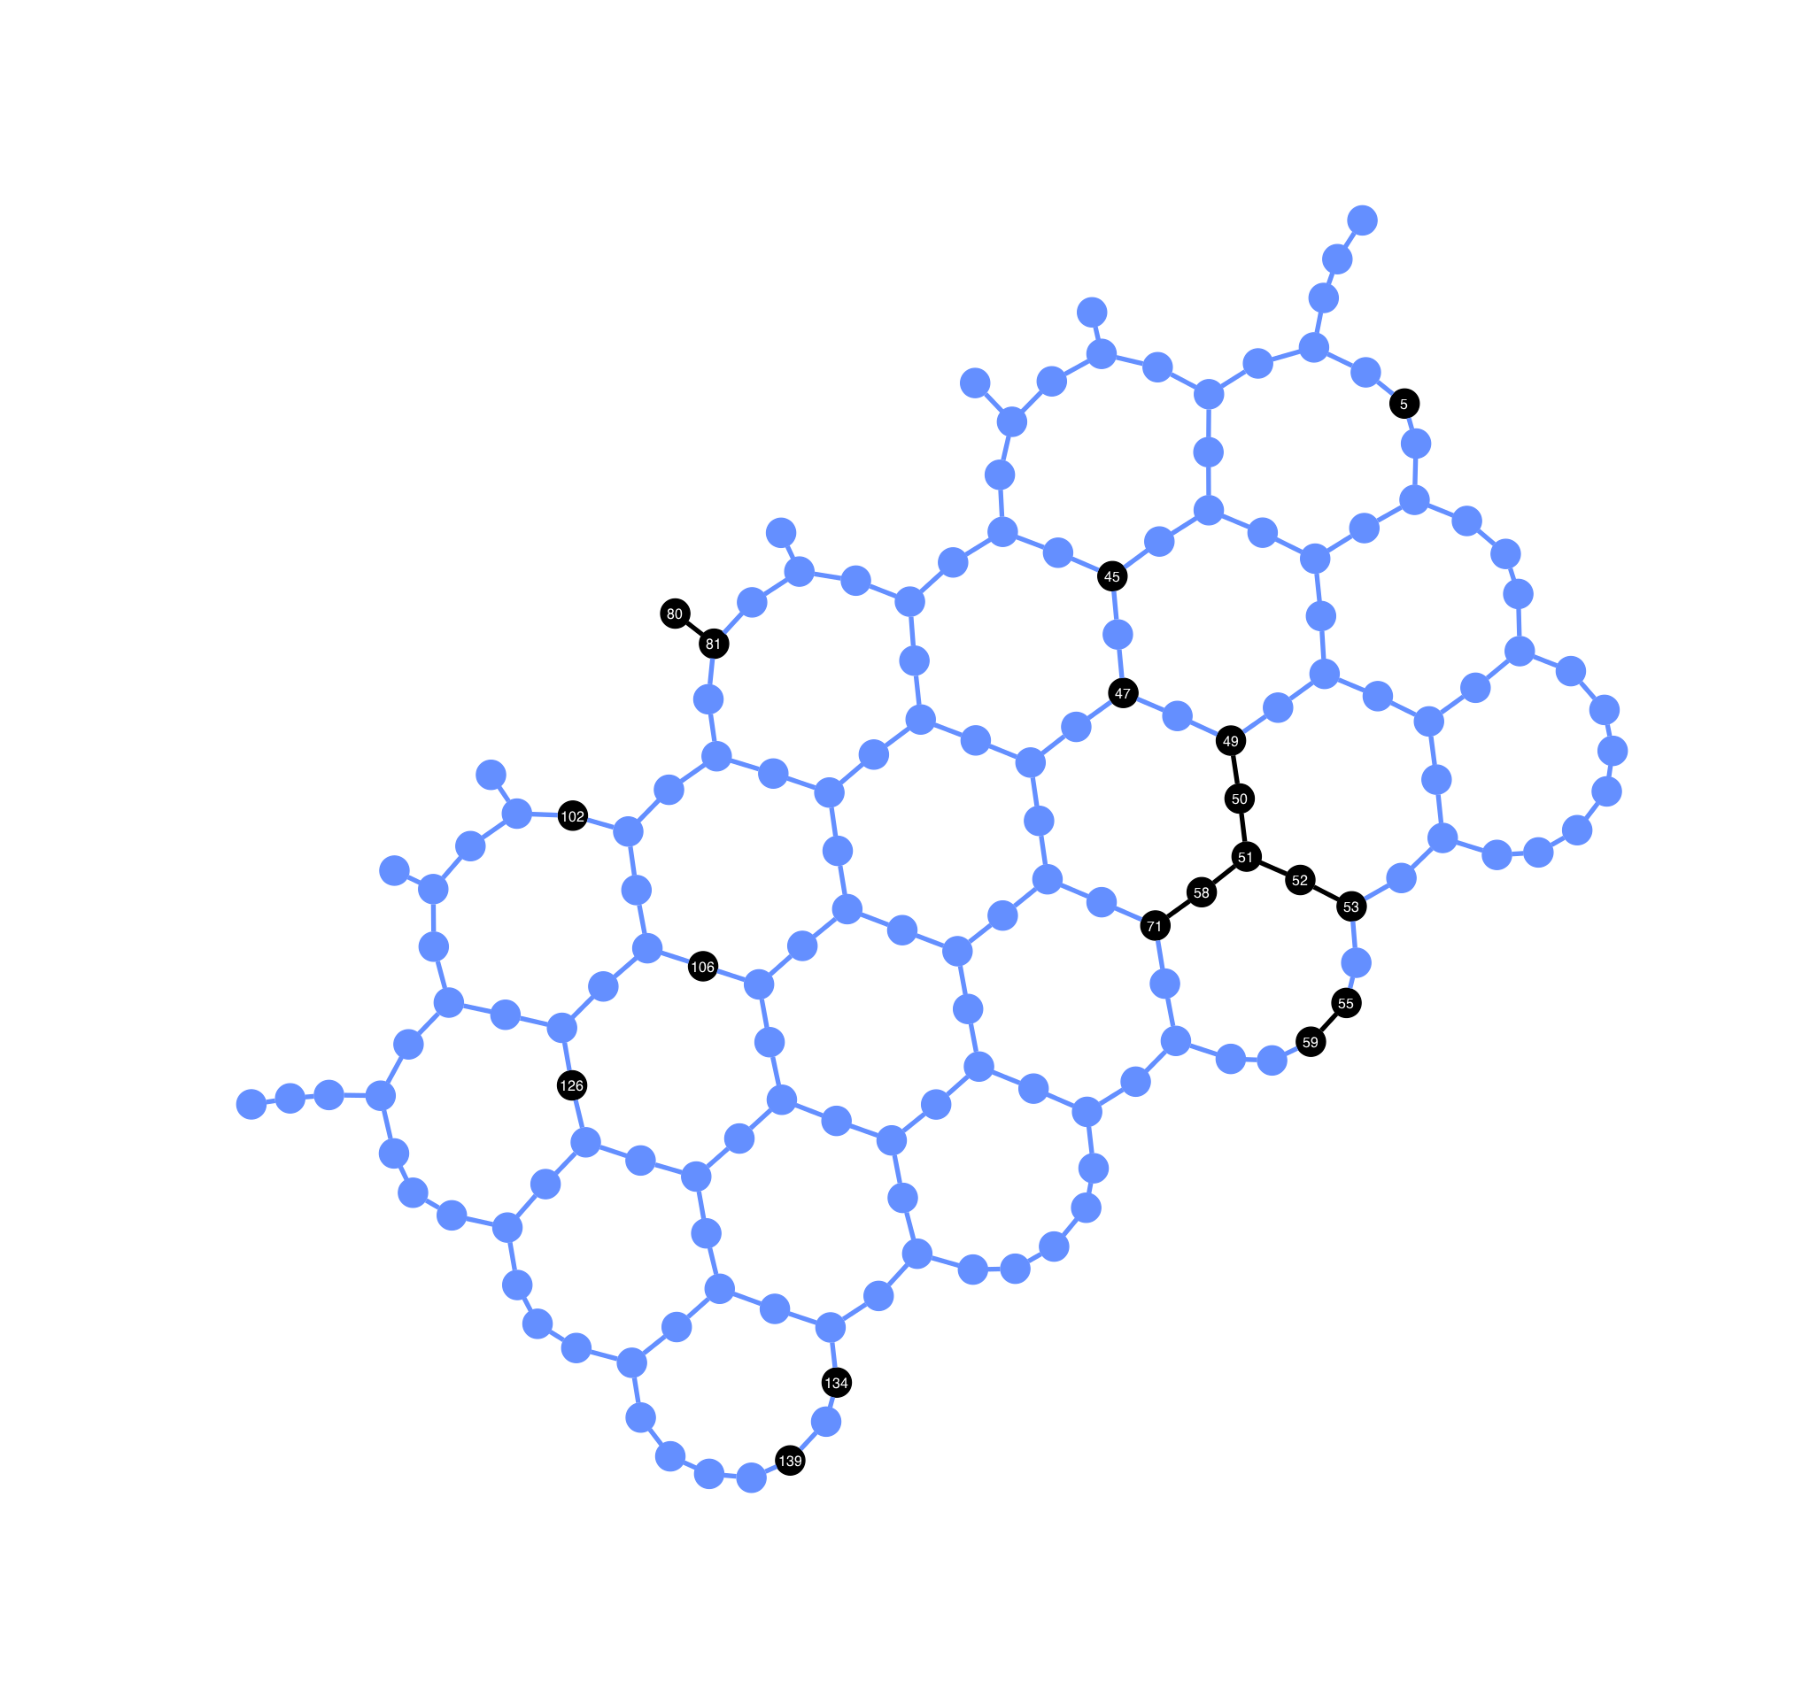
\includegraphics[width=\textwidth]{ibm_aachen_physical_circuit_layout_N55_a34.png} \\
  \small (a) $N=55$, $a=34$
\end{minipage} 
\begin{minipage}{0.3\textwidth}
  \centering
  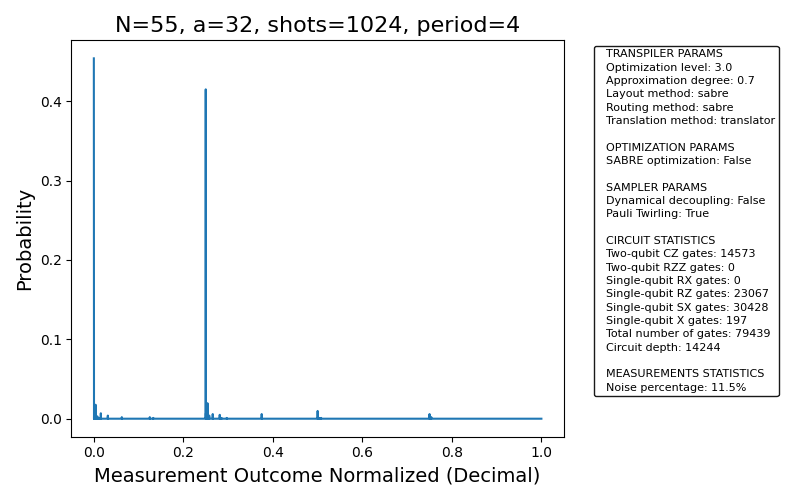
\includegraphics[width=\textwidth]{prob_dist_N55_a32_backend_ibmqpu.png} \\
\end{minipage} \\
\begin{minipage}{0.15\textwidth}
  \centering
  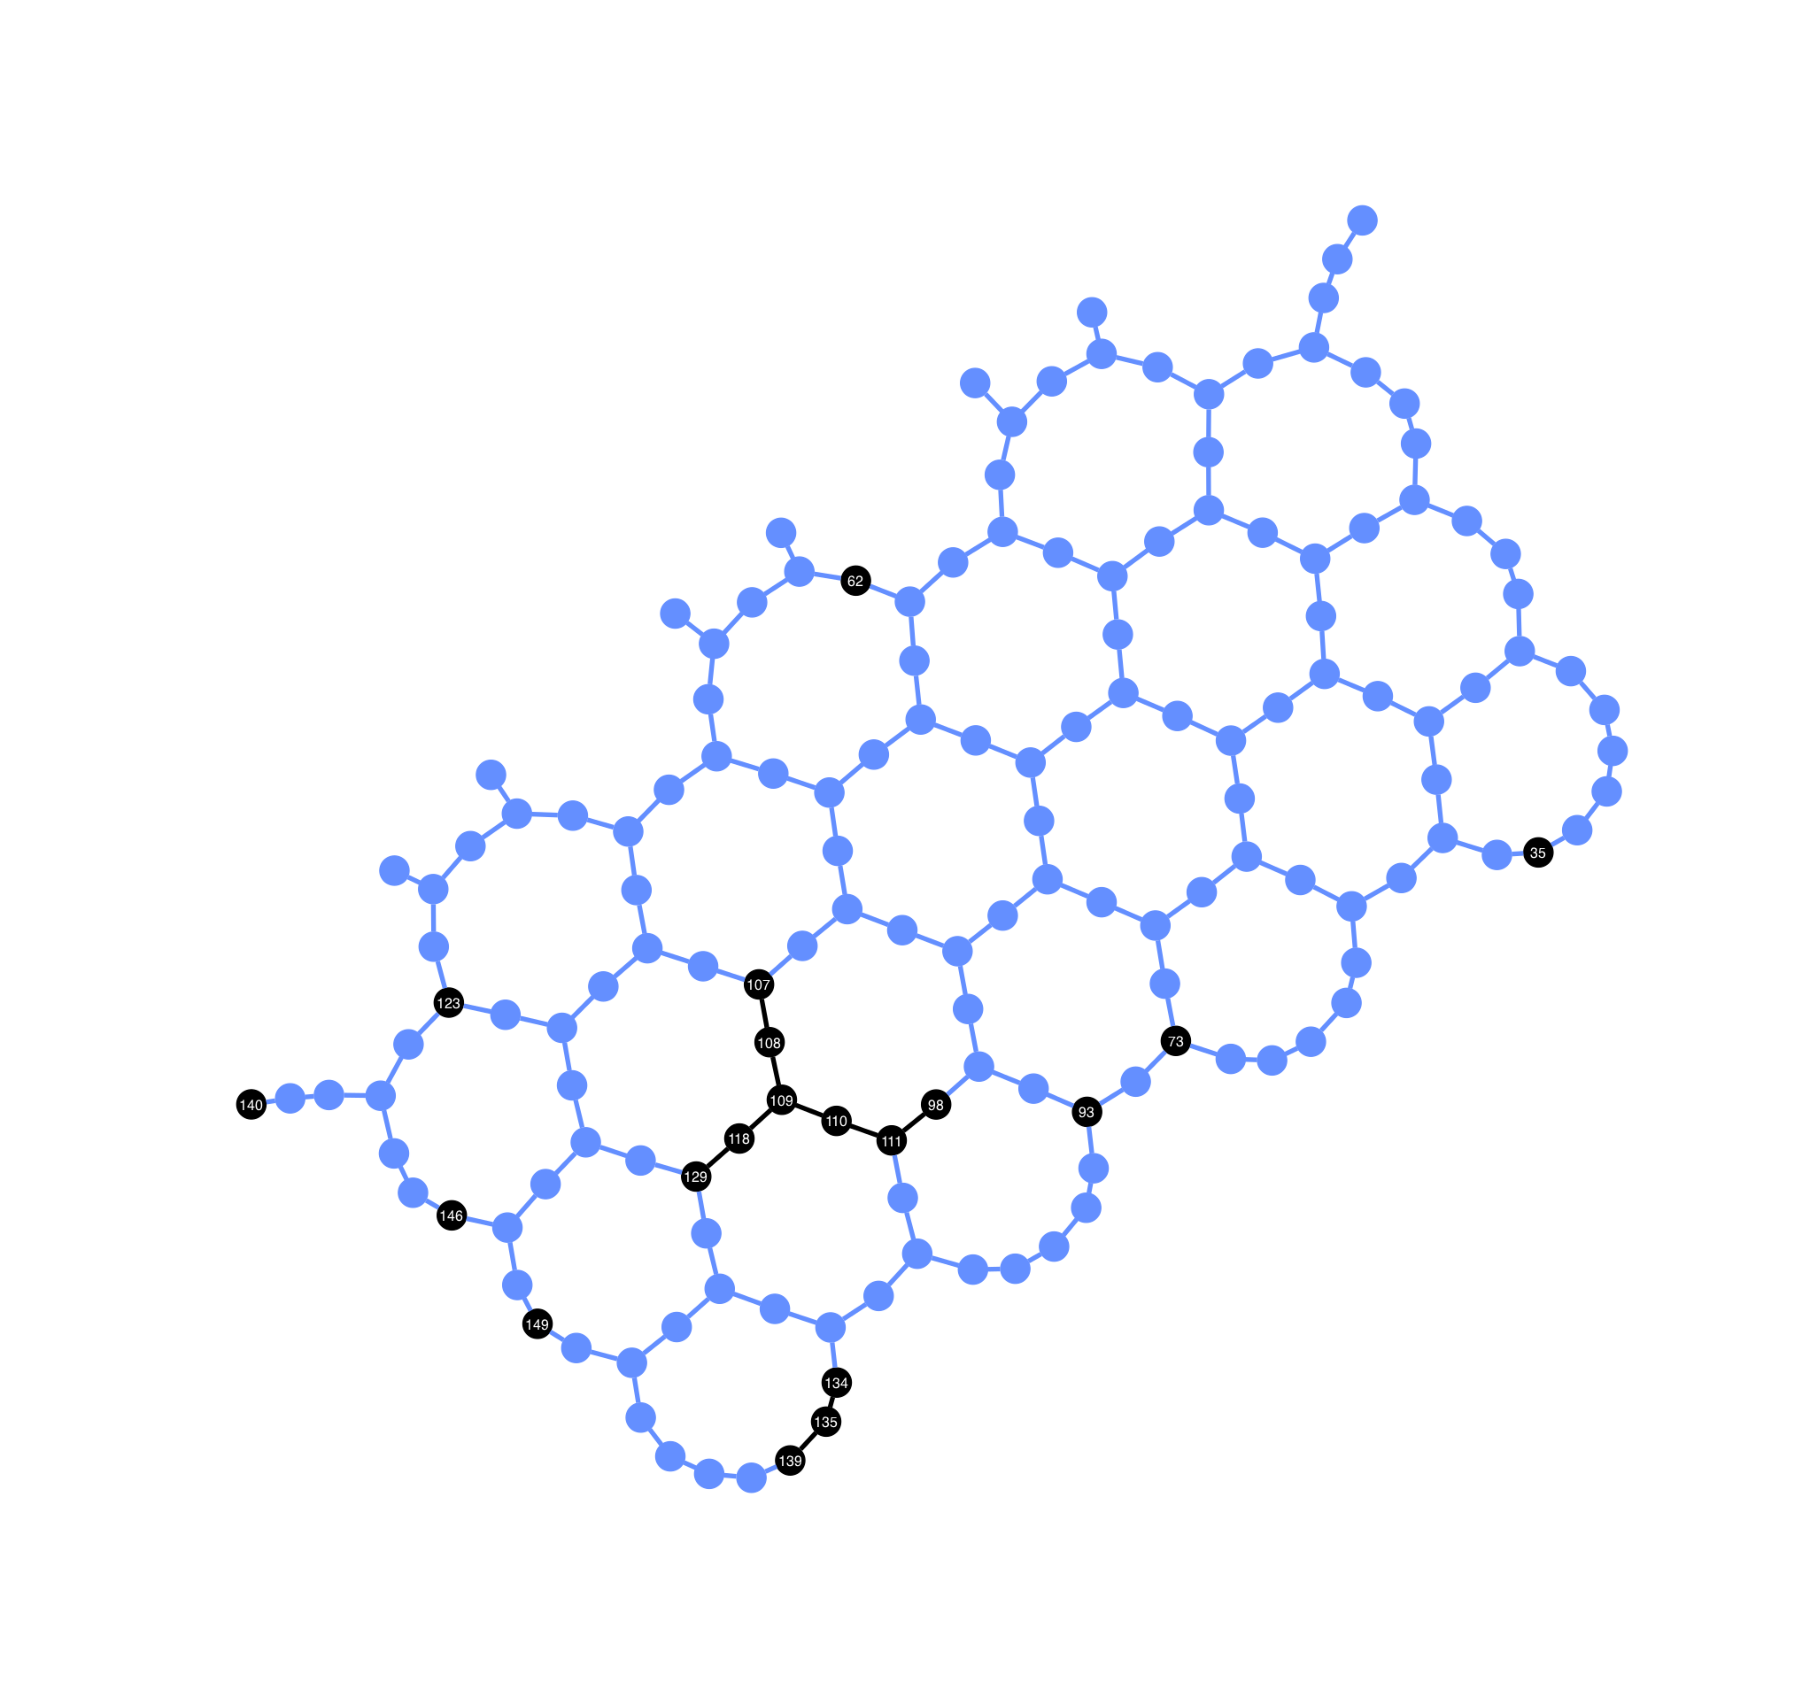
\includegraphics[width=\textwidth]{ibm_aachen_physical_circuit_layout_N55_a43.png} \\
  \small (b) $N=55$, $a=43$
\end{minipage} 
\begin{minipage}{0.3\textwidth}
  \centering
  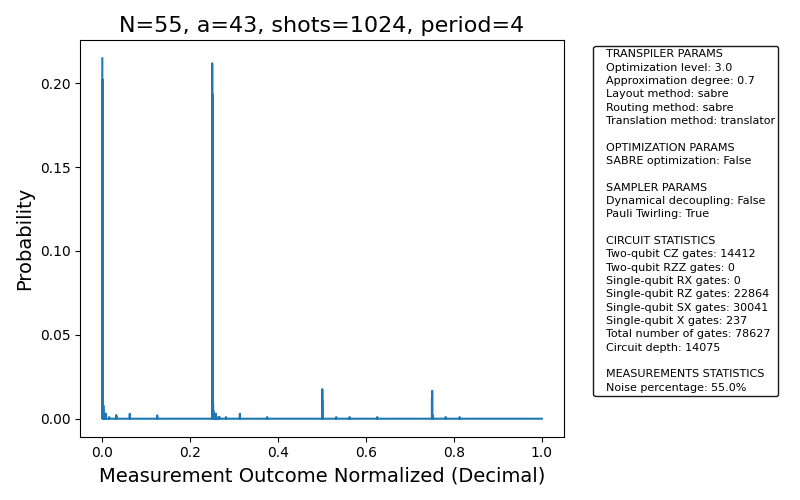
\includegraphics[width=\textwidth]{prob_dist_N55_a43_backend_ibmqpu.png} \\
\end{minipage} \\
\begin{minipage}{0.15\textwidth}
  \centering
  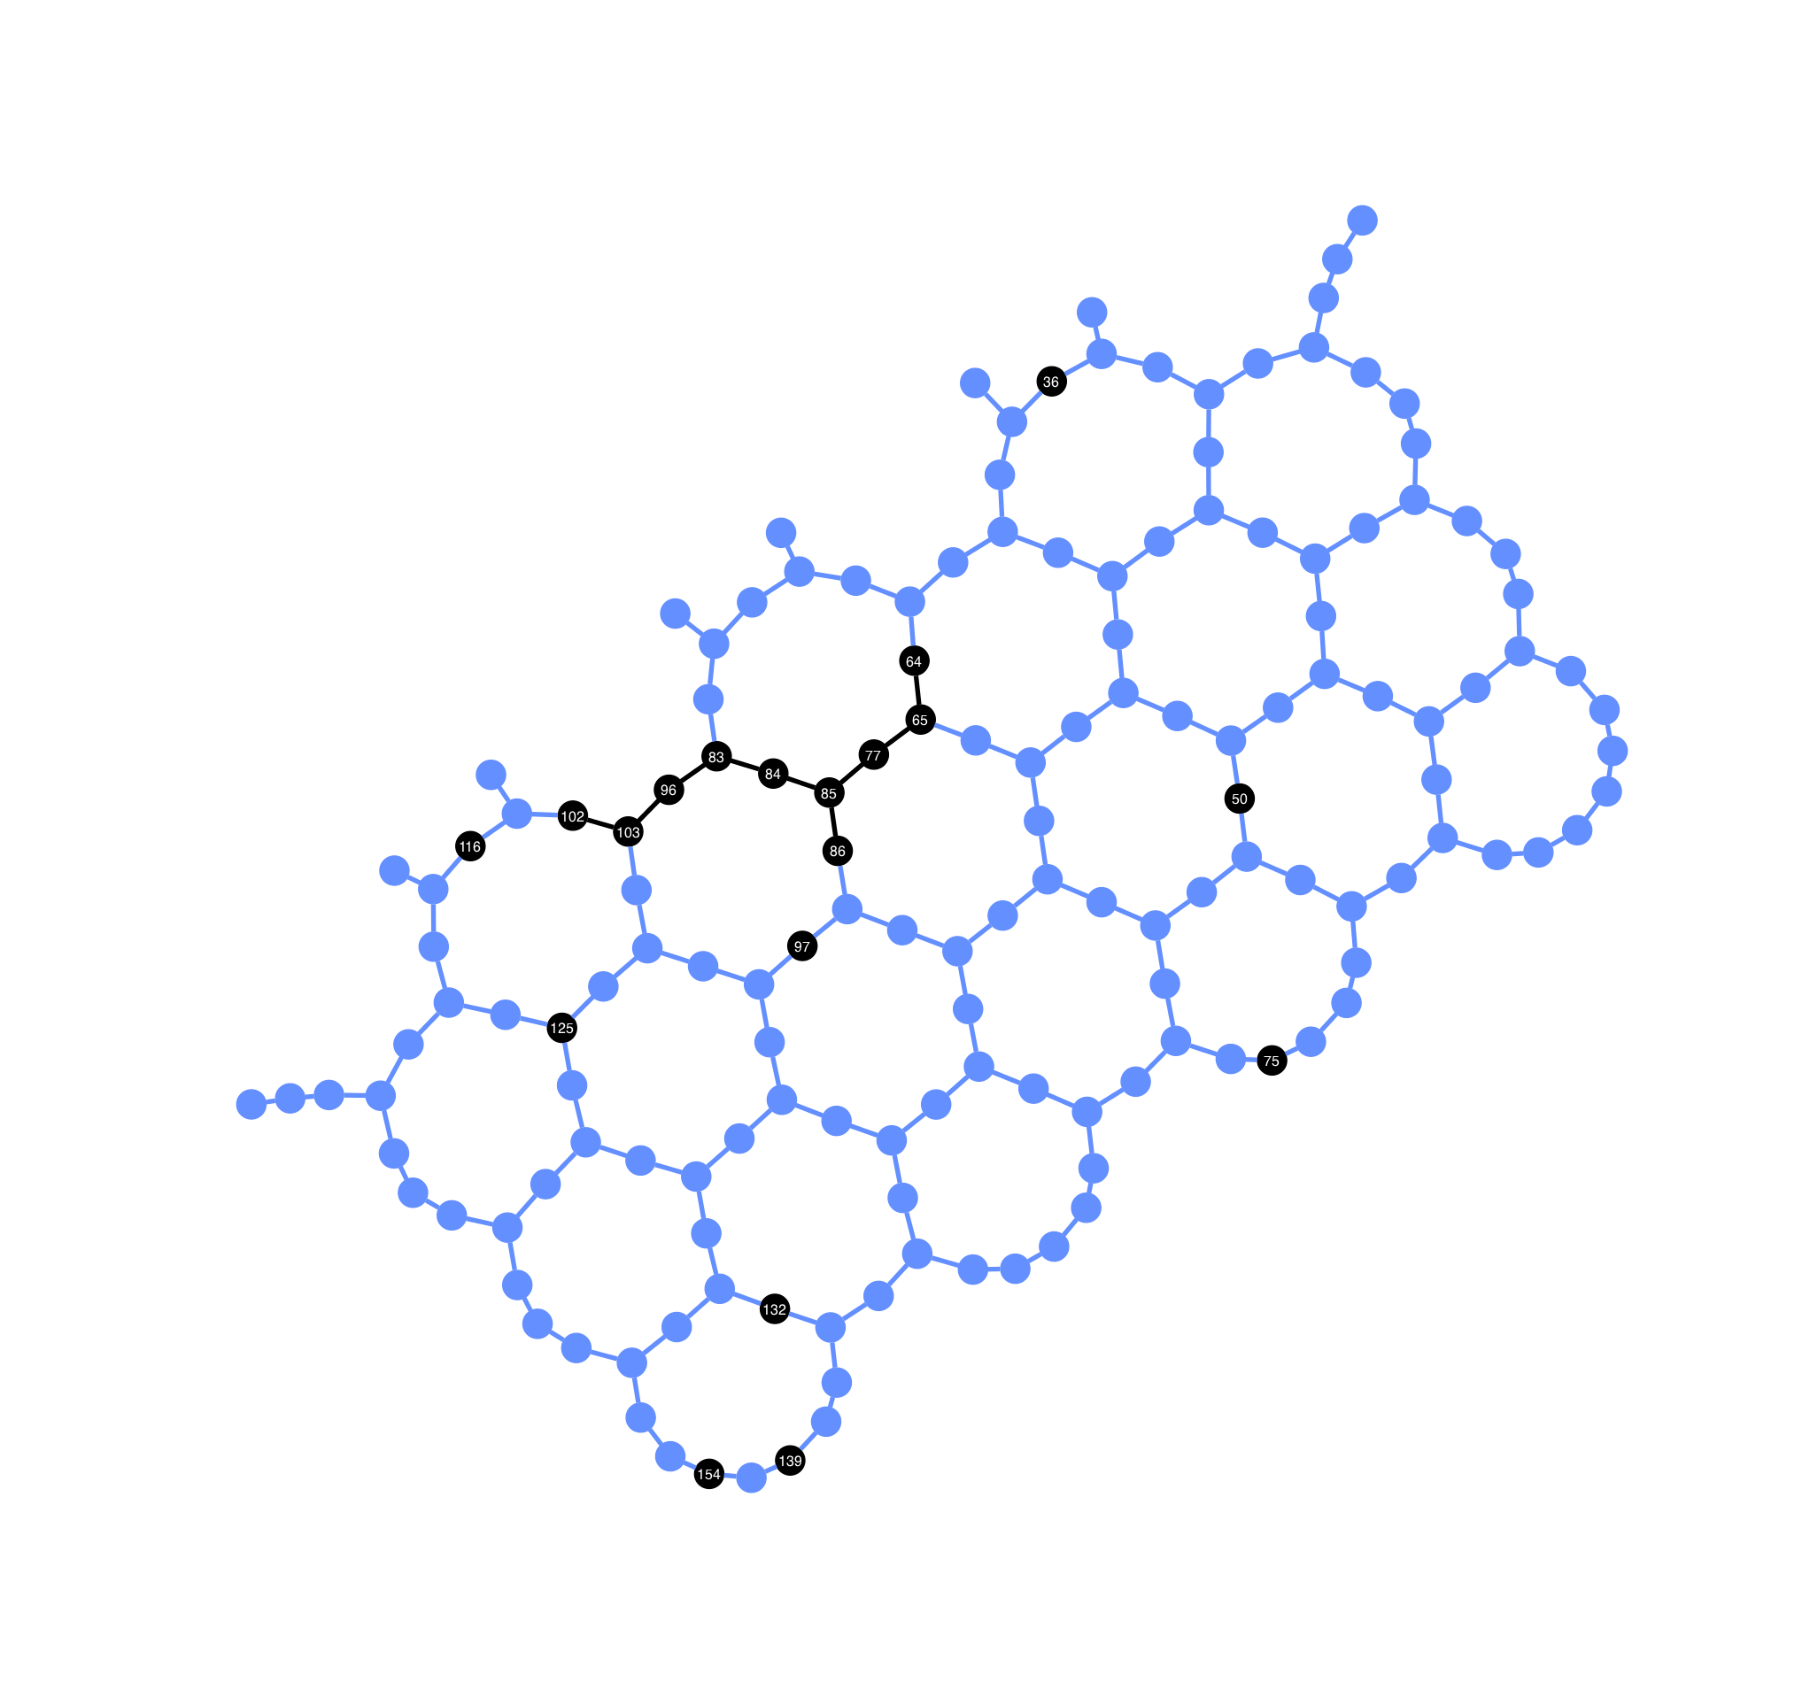
\includegraphics[width=\textwidth]{ibm_aachen_physical_circuit_layout_N55_a54.png} \\
  \small (c) $N=55$, $a=54$
\end{minipage} 
\begin{minipage}{0.3\textwidth}
  \centering
  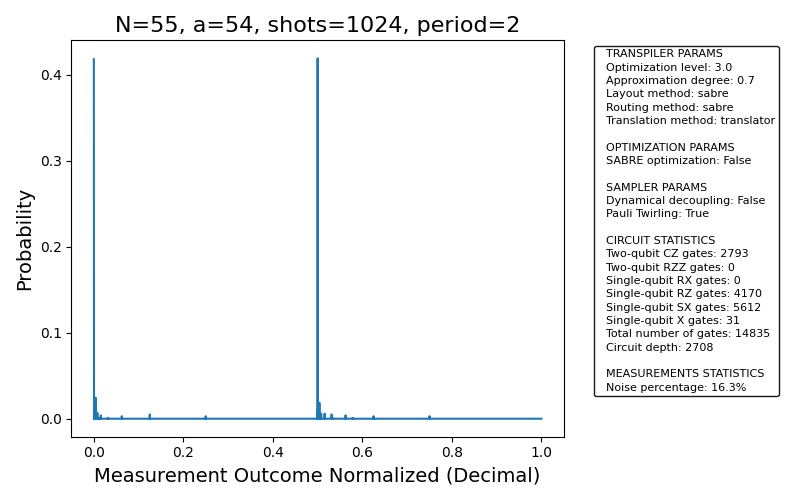
\includegraphics[width=\textwidth]{prob_dist_N55_a54_backend_ibmqpu.png} \\
\end{minipage} \\
\bottomrule
\end{tabular}
\caption{Summary Table of Probability Distributions for $N=55$ and a) $a=12$, b) $a=21$, c) $a=23$, d) $a=32$, e) $a=34$, f) $a=43$, and g) $a=54$, the only 7 $a$'s for which the total number of gates is \< 50,000 gates. $r=4$ in all cases, except $r=2$ for $a=21$ and $a=54$. For $a=54$ the correct non-trivial factors were found}
\label{tab:Factoring_N=55}
\end{figure}

% Creating the table for quantum circuit statistics
\begin{table*}[h]
\centering
\caption{Quantum Circuit Statistics for $N=57$ and Different $a$ Coefficients, transpiled and successfully executed in an \texttt{ibm\_aachen} QPU with Optimization Degree = 3, Approximation Factor = 0.7, and Pauli Twirling}
\label{tab:QC_statistics_N=57_all_a}
\begin{tabular}{rrrrrrrrrrr}
\toprule
{$a$} & r & {RX Gates} & {RZ Gates} & {SX Gates} & {X Gates} & {CZ Gates} & {RZZ Gates} & {Total Gates} & {Circuit Depth} & {Histogram Noise} \\
\midrule
2 & 18 & 0 & 150058 & 210092 & 1511 & 100605 & 0 & 537899 & 98288 & -- \\
4 &  9 & 0 & 155039 & 216480 & 1468 & 103706 & 0 & 554437 & 101234 & --  \\
5 &  18 & 0 & 154044 & 214057 & 1415 & 102035 & 0 & 547789 & 99487 & --  \\
7 &  3 & 0 & 125055 & 174430 & 1836 & 84400  & 0 & 450081 & 82001 & --  \\
8 &  6 & 0 & 147436 & 207160 & 1639 & 99530  & 0 & 529853 & 97120 & --  \\
10 &  18 & 0 & 145709 & 202668 & 1556 & 96995  & 0 & 520263 & 94657 & -- \\
11 &  6 & 0 & 145428 & 205146 & 1480 & 99044  & 0 & 525190 & 96693 & -- \\
13 & 18  & 0 & 153616 & 214271 & 1421 & 102386 & 0 & 548300 & 99927 & -- \\
14 & 18  & 0 & 154590 & 215664 & 1461 & 103191 & 0 & 552086 & 100785 & -- \\
16 & 9  & 0 & 155217 & 216668 & 1494 & 103521 & 0 & 554360 & 101081 & -- \\
17 & 18  & 0 & 151090 & 211148 & 1372 & 100937 & 0 & 540289 & 98420 & -- \\
\textbf{20} & \textbf{2} & \textbf{0} & \textbf{9929}   & \textbf{14399}  & \textbf{96}   & \textbf{7117}   & \textbf{0} & \textbf{37146}  & \textbf{6992} & \textbf{19.3\%} \\
22 &  18 & 0 & 153095 & 213698 & 1552 & 102085 & 0 & 546836 & 99608 & -- \\
23 &  18 & 0 & 153045 & 213893 & 1470 & 102406 & 0 & 547592 & 99954 & -- \\
25 &  9 & 0 & 151890 & 210513 & 1431 & 100419 & 0 & 539544 & 97885 & -- \\
26 & 6 & 0 & 146254 & 205214 & 1466 & 98969  & 0 & 525805 & 96445 & -- \\
28 & 9  & 0 & 150352 & 210133 & 1413 & 100494 & 0 & 537867 & 98127 & -- \\
29 &  18 & 0 & 151741 & 211981 & 1372 & 101196 & 0 & 542085 & 98696 & -- \\
31 & 6  & 0 & 148426 & 209586 & 1595 & 101553 & 0 & 536955 & 99212 & -- \\
32 &  18 & 0 & 152732 & 214500 & 1487 & 102834 & 0 & 548719 & 100417 & -- \\
34 &  18 & 0 & 152184 & 211835 & 1351 & 100990 & 0 & 542202 & 98520 & -- \\
35 &  18 & 0 & 135616 & 188128 & 1701 & 90164  & 0 & 484400 & 87693 & -- \\
\textbf{37} & \textbf{2} & \textbf{0} & \textbf{11007}  & \textbf{15716}  & \textbf{112}  & \textbf{7649}   & \textbf{0} & \textbf{40428}  & \textbf{7494} & \textbf{17.0\%}  \\
40 &  18 & 0 & 150210 & 211526 & 1509 & 101733 & 0 & 541489 & 99411 & -- \\
41 & 18  & 0 & 153221 & 213952 & 1483 & 102328 & 0 & 547624 & 99900 & -- \\
43 &  9 & 0 & 150764 & 211621 & 1456 & 101718 & 0 & 542089 & 99494 & -- \\
44 & 18 & 0 & 149231 & 209170 & 1478 & 100117 & 0 & 535248 & 97709 & -- \\
46 & 6 & 0 & 144019 & 203294 & 1592 & 98177  & 0 & 520511 & 95809 & -- \\
47 & 18  & 0 & 153145 & 214086 & 1469 & 102691 & 0 & 548423 & 100290 & -- \\
49 & 3  & 0 & 149566 & 210474 & 1469 & 101475 & 0 & 538484 & 99012 & -- \\
50 & 6  & 0 & 149295 & 209577 & 1558 & 101115 & 0 & 536870 & 98706 & -- \\
52 &  18 & 0 & 151506 & 212377 & 1533 & 101885 & 0 & 543779 & 99671 & -- \\
53 & 18  & 0 & 152997 & 214160 & 1495 & 102465 & 0 & 547775 & 99938 & -- \\
55 &  9 & 0 & 149761 & 211135 & 1626 & 101400 & 0 & 540333 & 99115 & -- \\
\textbf{56} &\textbf{2} & \textbf{0} & \textbf{7840}   & \textbf{11695}  & \textbf{61}   & \textbf{5839}   & \textbf{0} & \textbf{29938}  & \textbf{5723} & \textbf{13.7\%}  \\
\bottomrule
\end{tabular}
\end{table*}


\begin{figure}[h]
\centering
\begin{tabular}{p{0.45\textwidth}}
\toprule
\begin{minipage}{0.1\textwidth}
  \centering
  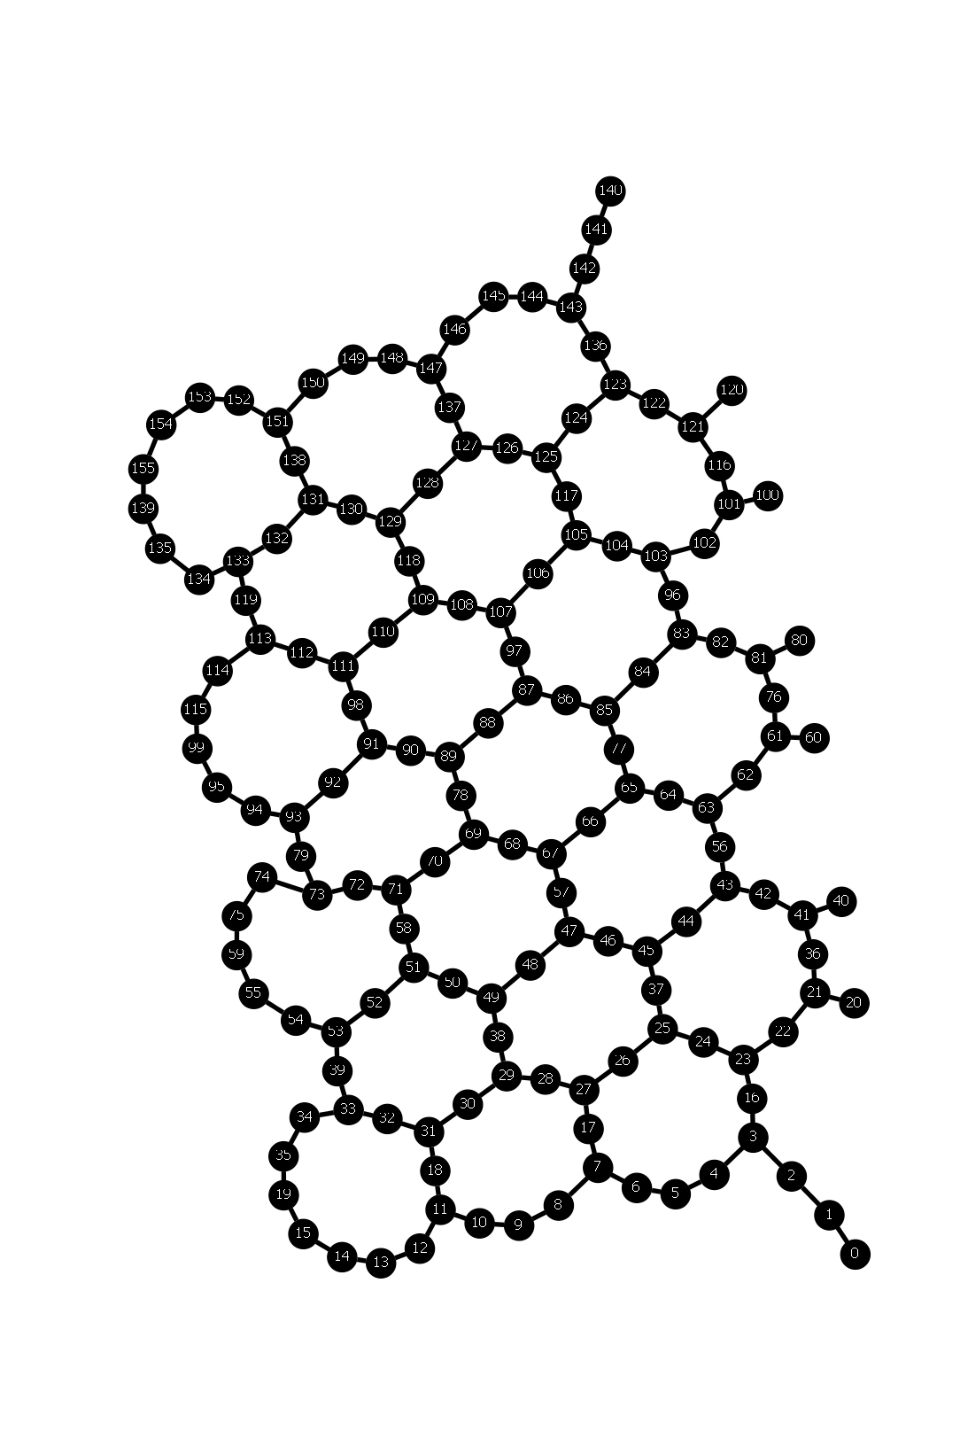
\includegraphics[width=\textwidth]{ibm_aachen_physical_circuit_layout_N57_a20.png} \\
  \small (a) $N=57$, $a=20$
\end{minipage} 
\begin{minipage}{0.3\textwidth}
  \centering
  \includegraphics[width=\textwidth]{prob_dist_N57_a20_backend_ibmqpu.png} \\
\end{minipage} \\
\begin{minipage}{0.1\textwidth}
  \centering
  \includegraphics[width=\textwidth]{ibm_aachen_physical_circuit_layout_N57_a37.png} \\
  \small (b) $N=57$, $a=37$
\end{minipage} 
\begin{minipage}{0.3\textwidth}
  \centering
  \includegraphics[width=\textwidth]{prob_dist_N57_a37_backend_ibmqpu.png} \\
\end{minipage} \\
\begin{minipage}{0.1\textwidth}
  \centering
  \includegraphics[width=\textwidth]{ibm_aachen_physical_circuit_layout_N57_a56.png} \\
  \small (c) $N=57$, $a=56$
\end{minipage} 
\begin{minipage}{0.3\textwidth}
  \centering
  \includegraphics[width=\textwidth]{prob_dist_N57_a56_backend_ibmqpu.png} \\
\end{minipage} \\
\bottomrule
\end{tabular}
\caption{Circuit layout and Probability Distributions for $N=57$ and a) $a=20$, b) $a=37$, and c) $a=56$.}
\label{tab:Factoring_N=57}
\end{figure}

\begin{table*}[!htbp]
\centering
\caption{Quantum Circuit Statistics for $N=65$ and Different $a$ Coefficients, transpiled and successfully executed in an \texttt{ibm\_aachen} QPU with Optimization Degree = 3, Approximation Factor = 0.7, and Pauli Twirling}
\label{tab:QC_statistics_N=65_all_a}
\begin{tabular}{rrrrrrrrrrr}
\toprule
$a$ & r & RX Gates & RZ Gates & SX Gates & X Gates & CZ Gates & RZZ Gates & Total Gates & Circuit Depth & Histogram Noise\\
\midrule
2 &  12 & 501779 & 0 & 0 & 801352 & 1067092 & 3814 & 2745207 & 494956& -- \\
3 &  12 & 493606 & 0 & 0 & 790288 & 1051119 & 3712 & 2702897 & 486471& -- \\
4 &  6 & 500675 & 0 & 0 & 801224 & 1064951 & 3557 & 2740934 & 493856& -- \\
6 &  12 & 494715 & 0 & 0 & 790745 & 1052929 & 3690 & 2707979 & 488012& -- \\
7 &  12 & 388444 & 0 & 0 & 622867 & 821824 & 5455 & 2133977 & 380830& -- \\
8 &  4 & 62192 & 0 & 0 & 98891 & 131754 & 448 & 339705 & 61398& -- \\
9 &  6 & 494455 & 0 & 0 & 790234 & 1051727 & 3722 & 2706468 & 487558& -- \\
11 & 12  & 493703 & 0 & 0 & 786674 & 1048440 & 3528 & 2698068 & 486934& -- \\
12 &  4 & 60169 & 0 & 0 & 94070 & 126971 & 472 & 326722 & 59410& -- \\
\textbf{14} & \textbf{2}  & \textbf{29627} & \textbf{0} & \textbf{0} & \textbf{46570} & \textbf{62348} & \textbf{255} & \textbf{161286} & \textbf{29280} & \textbf{56.3 \%} \\
16 &  3 & 499119 & 0 & 0 & 801622 & 1063634 & 3707 & 2737053 & 492187& -- \\
17 &  12 & 490198 & 0 & 0 & 785547 & 1043214 & 3586 & 2684924 & 483500& -- \\
18 & 4  & 59563 & 0 & 0 & 94725 & 126267 & 481 & 325607 & 58805& -- \\
19 & 12  & 492384 & 0 & 0 & 788748 & 1047422 & 3739 & 2697183 & 485807& -- \\
21 &  4 & 62024 & 0 & 0 & 98082 & 131503 & 502 & 338739 & 61248& -- \\
22 & 12  & 487345 & 0 & 0 & 774785 & 1020404 & 4780 & 2648215 & 480529& -- \\
23 &  12 & 483761 & 0 & 0 & 765402 & 1010165 & 4824 & 2623290 & 477198& -- \\
24 &  12 & 493646 & 0 & 0 & 778364 & 1030721 & 4825 & 2673210 & 486868& -- \\
27 & 4  & 59479 & 0 & 0 & 91739 & 122869 & 586 & 319407 & 58768& -- \\
28 &  12 & 488873 & 0 & 0 & 771352 & 1021096 & 4715 & 2648383 & 482237& -- \\
29 & 6  & 491283 & 0 & 0 & 779478 & 1028541 & 4639 & 2667700 & 484345& -- \\
31 &  4 & 60512 & 0 & 0 & 93209 & 125114 & 528 & 324487 & 59770& -- \\
32 & 12  & 408765 & 0 & 0 & 650431 & 853605 & 5862 & 2227898 & 401711& -- \\
33 &  12 & 488508 & 0 & 0 & 772836 & 1020430 & 4684 & 2648578 & 481685& -- \\
34 &  4 & 60920 & 0 & 0 & 96113 & 126928 & 596 & 329928 & 60047& -- \\
36 & 6  & 498448 & 0 & 0 & 791834 & 1043665 & 5019 & 2707576 & 491257& -- \\
37 & 12  & 502659 & 0 & 0 & 799816 & 1053434 & 4853 & 2732195 & 495348& -- \\
38 & 4  & 59175 & 0 & 0 & 92340 & 122867 & 613 & 319439 & 58476& -- \\
41 & 12  & 500031 & 0 & 0 & 794740 & 1048339 & 4698 & 2717560 & 492778& -- \\
42 & 12  & 493457 & 0 & 0 & 784074 & 1033628 & 4836 & 2680857 & 486533& -- \\
43 &  12 & 498278 & 0 & 0 & 794292 & 1059431 & 3758 & 2724257 & 491618& -- \\
44 & 4  & 61510 & 0 & 0 & 97481 & 130095 & 463 & 335401 & 60707& -- \\
46 &  12 & 488687 & 0 & 0 & 782823 & 1040982 & 3638 & 2678352 & 481904& -- \\
47 & 4  & 58237 & 0 & 0 & 92234 & 123235 & 516 & 317657 & 57527& -- \\
48 & 12  & 496332 & 0 & 0 & 794592 & 1057297 & 3639 & 2718189 & 489201& -- \\
49 & 6  & 489532 & 0 & 0 & 783312 & 1042643 & 3556 & 2681457 & 482625& -- \\
\textbf{51} & \textbf{2} & \textbf{30524} & \textbf{0} & \textbf{0} & \textbf{48562} & \textbf{64816} & \textbf{211} & \textbf{166981} & \textbf{30129} & \textbf{55.3\%} \\
53 &  4 & 59830 & 0 & 0 & 94526 & 126313 & 549 & 326108 & 59108& -- \\
54 & 12  & 490829 & 0 & 0 & 776372 & 1025957 & 4816 & 2661871 & 484122& -- \\
56 & 6  & 496250 & 0 & 0 & 785113 & 1037350 & 4851 & 2691157 & 489460& -- \\
57 &  4 & 60684 & 0 & 0 & 93657 & 125149 & 515 & 325409 & 59921& -- \\
58 & 12  & 489736 & 0 & 0 & 768783 & 1020456 & 4908 & 2647082 & 483212& -- \\
59 &  12 & 490126 & 0 & 0 & 777376 & 1026004 & 4789 & 2661668 & 483385& -- \\
61 & 3  & 498438 & 0 & 0 & 795187 & 1045814 & 4761 & 2712417 & 491412& -- \\
62 & 12  & 493043 & 0 & 0 & 781927 & 1031655 & 4775 & 2676686 & 486280& -- \\
63 & 12  & 497617 & 0 & 0 & 791111 & 1042877 & 4781 & 2704992 & 490742& -- \\
\textbf{64} &  \textbf{2} & \textbf{29012} & \textbf{0} & \textbf{0} & \textbf{45589} & \textbf{60240} & \textbf{262} & \textbf{157026} &\textbf{ 28587}& -- \\
\bottomrule
\end{tabular}
\end{table*}

\begin{figure}[!htbp]
\begin{tabular}
\centering
\begin{minipage}{0.1\textwidth}
  \centering
  \includegraphics[width=\textwidth]{ibm_aachen_physical_circuit_layout_N65_a14.png} \\
  \small (a) $N=65$, $a=14$
\end{minipage} 
\begin{minipage}{0.3\textwidth}
  \centering
  \includegraphics[width=\textwidth]{prob_dist_N65_a14_backend_ibmqpu.png} \\
\end{minipage} \\
\begin{minipage}{0.1\textwidth}
  \centering
  \includegraphics[width=\textwidth]{ibm_aachen_physical_circuit_layout_N65_a51.png} \\
  \small (b) $N=65$, $a=51$
\end{minipage} 
\begin{minipage}{0.3\textwidth}
  \centering
  \includegraphics[width=\textwidth]{prob_dist_N65_a51_backend_ibmqpu.png} \\
\end{minipage} \\
\bottomrule
\end{tabular}
\caption{Circuit layout and Probability Distributions for $N=65$ and a) $a=14$, and b) $a=51$.}
\label{tab:Factoring_N=65}
\end{figure}


\subsubsection{Circuit Performance Dependence on the particular QPU}

We started performing most of our studies with IBM Kyiv QPU, having achieved already the capability to factorize $N=51$ (see Fig. \ref{fig:Kyivs_reincarnation}). However, on March 18th, 2025, the machine was no longer available, and we had to use other machines. Unfortunately, despite having similar specifications and theoretical performance, it was not possible to reproduce the results. It was hypothesized that this was due to less noisy qubits, or mapping into the circuit layout, but the coherence times are very similar. 
To address this issue, \texttt{ibm\_Kyiv}'s circuit layout was literally "implanted" in four other computers (\texttt{ibm\_Brisbane}, \texttt{ibm\_Sherbrooke}, \texttt{ibm\_Brussels} and \texttt{ibm\_Strasbourg}), which means that the circuit topology was exactly the same. Despite this, results were dramatically different (Table \ref{Kyiv_reincarnation} ). 

\texttt{ibm\_Kyiv}'s depth of 5,309 is approximately five times smaller than the others (25,325--25,326), which are nearly identical. This suggests that \texttt{ibm\_Kyiv}'s circuit was optimized through a far more efficient transpilation, reduced swap gate insertion, or a topology-aligned qubit mapping. The uniformity among the other QPUs indicates a more standardized compilation approach, with minor variations possibly due to QPU-specific connectivity.

In terms of the total number of gates \texttt{ibm\_Kyiv}'s 46,447 gates are significantly lower than \texttt{ibm\_Strasbourg}'s 189,416 to \texttt{ibm\_Brisbane}'s 209,487. The 10--15\% variation among the other QPUs suggests differences in transpilation or routing overhead. RZ gates dominate (\~40\% of the total), followed by SX (~25--30\%), ECR (~12--15\%), and X (\< 5\%) gates, reflecting the structure of Shor's algorithm, which relies heavily on quantum Fourier transforms and modular arithmetic.

All QPUs use the Eagle r3 architecture with the basis gate set \{ecr, id, rz, sx, x\}. Thus, differences arise from transpilation, and are not due to the  set of native gates.

In terms of the error rates \texttt{ibm\_Sherbrooke} and \texttt{ibm\_Brisbane} have the lowest error rates, while \texttt{ibm\_Strasbourg} has the highest. \texttt{ibm\_Kyiv}'s moderate errors do not explain either its compact circuit. Among the others, \texttt{ibm\_Sherbrooke}'s lower layered error may reduce its gate count by minimizing swap gates. \texttt{ibm\_Strasbourg}'s higher errors may increase routing overhead, but its has a lower gate count which suggests that transpilation dominates.

Coherence times and number of qubits are pretty uniform (100--150 \si{\micro\second}) and number of qubit is the same (127), so they cannot contribute to observed differences either.

CLOPS ranges from 150K to 220K, with Kyiv's having a moderate CLOPS (200K). Therefore it does not explain either its efficiency.

After all these analyses, we discard all possible causes except that \texttt{ibm\_Kyiv}'s more compact circuit may be likely due to a very optimized transpilation. This highlights the importance of transpilation with NISQ and shows directions to  enhance circuit efficiency.

\begin{table*}[h]
\centering
\caption{Comparison of Circuit Parameters Across Different QPUs For $N=51$, and $a=4$}
\label{Kyiv_reincarnation}
\resizebox{\textwidth}{!}{%
\begin{tabular}{@{} l *{6}{S[table-format=5.0]} @{}}
\toprule
\textbf{QPU} & \textbf{Two-qubit ECR Gates} & \textbf{Single-qubit RZ Gates} & \textbf{Single-qubit SX Gates} & \textbf{Single-qubit X Gates} & \textbf{Total Gates} & \textbf{Circuit Depth} \\
\midrule
Kyiv         & 5502  & 21554 & 14155 & 621   & 46447  & 5309  \\
Brisbane     & 25741 & 95992 & 61864 & 4710  & 209487 & 25326 \\
Sherbrooke   & 25743 & 91728 & 59566 & 5897  & 204124 & 25326 \\
Brussels     & 25740 & 96312 & 59777 & 6296  & 209298 & 25325 \\
Strasbourg  & 25743 & 81894 & 49707 & 10896 & 189416 & 25326 \\
\bottomrule
\end{tabular}%
}
\end{table*}

\begin{figure}[!htbp]
\centering
\begin{tabular}{p{0.45\textwidth}}
\toprule
\begin{minipage}{0.15\textwidth}
  \centering
  \includegraphics[width=\textwidth]{ibm_kyiv_physical_circuit_layout.png} \\
  \small (a) $N=51$, $a=4$
\end{minipage} 
\begin{minipage}{0.3\textwidth}
  \centering
  \includegraphics[width=\textwidth]{prob_dist_N51_a4_backend_ibmqpu.png} \\
\end{minipage} \\
\bottomrule
\end{tabular}
\caption{Circuit layout and Probability Distributions for $N=51$ and a) $a=4$ in Kyiv QPU. Same circuit layout was implanted in Brisbane, Sherbrooke, Brussels and Strasbourg QPUs, but it did not work.}
\label{fig:Kyivs_reincarnation}
\end{figure}

\subsubsection{Optimizing of Shor’s Algorithm for Real Quantum Hardware: Classical Preprocessing for Maximum Factorable N, the Optima $a$ Values}

In this section, our primary objective is to investigate how far we could extend the factorization capabilities of Shor’s algorithm beyond the brute force approach of trying $a$ values randomly. To do this we use the most powerful QPU available to us \texttt{ibm\_aachen}'s quantum processor, which features 156 qubits and employs a Heron r2-type QPU. 
Ideally, when executed on quantum hardware, Shor’s algorithm would randomly test multiple values of $a$ until it identifies one that yields a useful period, ideally, the smallest possible period ($r=2$). However, due to current hardware limitations, this approach is highly time-consuming and impractical.
In the previous sections, we adopted a methodological approach: for each value of $N$ to be factored, we generated all coprime values of $N$, and transpiled each of them in the corresponding quantum circuit. Once we identified the $a$ that produced the lowest circuit depth number, we executed that circuit on the real \texttt{ibm\_aachen} quantum processor.
However, as $N$ increased, the process became extremely time-consuming. For example, when factoring $N=57$, we evaluated 35 coprime values of $a$, specifically (2, 4, 5, 7, 8, 10, 11, 13, 14, 16, 17, 20, 22, 23, 25, 26, 28, 29, 31, 32, 34, 35, 37, 40, 41, 43, 44, 46, 47, 49, 50, 52, 53, 55, 56). On average, each transpilation required approximately two hours, resulting in a total of nearly 70 hours to identify the optimal $a$.
This exhaustive process becomes increasingly unsustainable for larger numbers, particularly given current hardware constraints. Despite working with a 156-qubit machine, the practical limitations of circuit depth and gate fidelity meant that we remained restricted to relatively small integers, far below those relevant to real-world cryptographic applications.
To overcome this bottleneck, based on our previous experience of transpiling all the admissible values of $a$, we realized that when searching for the $a$ that produces the lowest circuit depth a pattern appeared. As you can observe in tables \ref{tab:QC_statistics_N=55_all_a}, \ref{tab:QC_statistics_N=57_all_a}, and \ref{tab:QC_statistics_N=65_all_a}, the bolded lines mark the transpiled circuits that possess the lowest circuit depth, and for those the corresponding $r$ value is always \textbf{2}. So our objective was come up with a way to know in advance those $a$ values that produce periods (r) equal to 2, and that as a consequence generate circuits with the lowest circuit depth. To achieve this, we developed a classical pre-processing algorithm designed to identify values of $a$ that are more likely to yield the smallest possible period ($r = 2$). Specifically, the script computes the order $r$, the smallest positive integer such that \( a^r \equiv 1 \mod N \), for all values of a that are coprime to a given N. For example, when factoring $N = 111$, the algorithm identified three values of a (38, 73, and 110) that yielded the minimal period $r = 2.$ These values were then prioritized for circuit transpilation and execution. 
% Pseudocode
The pseudocode 4 outlines the steps of the $Order \ Finding  \ Algorithm$.

\begin{algorithm}
\caption{Order Finding Algorithm}
\begin{algorithmic}[]
\State \textbf{Input}: Integer \( N \), base \( a \)
\State \textbf{Output}: Order \( r \) or None

\For{\( a \) from 2 to \( N \)}
    \If{\( \gcd(a, N) = 1 \) (check if \( a \), \( N \) coprime)}
        \State \( v = 1 \)
        \For{\( r \) from 1 to \( N \)}
            \State \( v = (v \times a) \mod N \) (update \( v \) with mod mult)
            \If{\( v = 1 \) (detect order)}
                \State \textbf{Return}: \( r \)
            \Else (no order yet)
                \State \textbf{Return}: None
            \EndIf
            \If{\( r \neq \text{None} \) (process valid \( r \))}
                \If{\( r < r_{\text{min}} \) (find smallest order)}
                    \State \( r_{\text{min}} = r \)
                    \State \( p = [(a, r)] \)
                \Else (handle other orders)
                    \State \( r = r_{\text{min}} \)
                    \State \( p.\text{append}((a, r)) \)
                \EndIf
            \EndIf
        \EndFor
    \EndIf
\EndFor
\State \textbf{Return}: Failure (no order found)
\end{algorithmic}
\end{algorithm}


This optimization significantly reduced the number of quantum circuits that needed to be transpiled and executed. As a result, we were able to factor larger numbers, such as 111, 115, 123, directly on the hardware, demonstrating a more scalable and efficient approach to implement Shor’s algorithm within current technological limits. It is worth mentioning that for these values of $N$, SABRE optimization had to be activated in order to potentially reduce the circuit depth.

Using the above technique, Fig. \ref{fig:Factoring_N=123} shows the quantum circuit, circuit layout, and the probability distributions for the maximum value of $N$ we have been able to factor $N = 123$ for $a = 40$ and $a=80$ with and without Pauli Twirling and with and without SABRE optimization. 
\\
An interesting fact that has been observed in all the optimum circuits analyzed is that all the exponentiation blocks except the first one are equal to $[1 mod N]$ (e.g. Fig. \ref{fig:Factoring_N=123} (a) ) which is probably the reason of the significantly smaller number of gates, and significantly improved performance.

\begin{figure*}[!htbp]
    \centering

    % Primera fila con 3 subfiguras
    \begin{subfigure}{0.12\textwidth}
        \centering
        \includegraphics[width=\textwidth]{ibm_aachen_physical_circuit_layout_N123_a40_PT1_SO0.png}
        \caption{$N=123$, $a=40$}
    \end{subfigure}
    \hfill
    \begin{subfigure}{0.2\textwidth}
        \centering
        \includegraphics[width=\textwidth]{ibm_aachen_physical_circuit_layout_N123_a83_PT1_SO0.png}
        \caption{$N=123$, $a=83$}
    \end{subfigure}
    \hfill
    \begin{subfigure}{0.45\textwidth}
        \centering
        \includegraphics[width=\textwidth]{ibm_aachen_quantum_circuit_N123_a40.png}
        \caption{Quantum circuit $N=123$, $a=40$ (for $a=83$ only $1^{st}$ exponentiation block changes) }
    \end{subfigure}

    \vspace{0pt} % Espacio vertical entre filas

    % Segunda fila con 2 subfiguras
    \begin{subfigure}{0.37\textwidth}
        \centering
        \includegraphics[width=\textwidth]{prob_dist_N123_a40_backend_ibmqpu_PT1_SO1.png}
        \caption{$a=40$, Pauli Twirling, SABRE Optimization}
    \end{subfigure}
    \hfill
    \begin{subfigure}{0.37\textwidth}
        \centering
        \includegraphics[width=\textwidth]{prob_dist_N123_a83_backend_ibmqpu_PT1_SO1.png}
        \caption{$a=83$, Pauli Twirling, SABRE Optimization}
    \end{subfigure}

    \vspace{0pt}

    % Tercera fila con 2 subfiguras
    \begin{subfigure}{0.37\textwidth}
        \centering
        \includegraphics[width=\textwidth]{prob_dist_N123_a40_backend_ibmqpu_PT0_SO0.png}
        \caption{$a=40$, No Pauli Twirling, No SABRE Optimization}
    \end{subfigure}
    \hfill
    \begin{subfigure}{0.37\textwidth}
        \centering
        \includegraphics[width=\textwidth]{prob_dist_N123_a83_backend_ibmqpu_PT0_SO0.png}
        \caption{$a=83$, No Pauli Twirling, No SABRE Optimization}
    \end{subfigure}

    \vspace{0pt}

    % Cuarta fila con 2 subfiguras
    \begin{subfigure}{0.37\textwidth}
        \centering
        \includegraphics[width=\textwidth]{prob_dist_N123_a40_backend_ibmqpu_PT1_SO0.png}
        \caption{$a=40$, Pauli Twirling, No SABRE Optimization}
    \end{subfigure}
    \hfill
    \begin{subfigure}{0.37\textwidth}
        \centering
        \includegraphics[width=\textwidth]{prob_dist_N123_a83_backend_ibmqpu_PT1_SO0.png}
        \caption{$a=83$, Pauli Twirling, No SABRE Optimization}
    \end{subfigure}

    \vspace{0pt}

    % Quinta fila con 2 subfiguras
    \begin{subfigure}{0.37\textwidth}
        \centering
        \includegraphics[width=\textwidth]{prob_dist_N123_a40_backend_ibmqpu_PT0_SO1.png}
        \caption{$a=40$, No Pauli Twirling, SABRE Optimization}
    \end{subfigure}
    \hfill
    \begin{subfigure}{0.37\textwidth}
        \centering
        \includegraphics[width=\textwidth]{prob_dist_N123_a83_backend_ibmqpu_PT0_SO1.png}
        \caption{$a=83$, No Pauli Twirling, SABRE Optimization}
    \end{subfigure}

    \caption{Quantum circuit (top), and probability distributions for $N=123$ and $a=40$ (left column) and $a=83$ (right column): a-b) with PT and SO, c-d) without PT, without SO, e-f) with PT and without SO, and g-h) without PT and with SO.}
    \label{fig:Factoring_N=123}
\end{figure*}

\section{Discussion}

The implementation and evaluation of Shor’s algorithm presented in this report illustrates its theoretical power and its current practical limitations. While Shor’s algorithm promises exponential speedup over classical algorithms for integer factorization —in principle a direct threat to RSA-based cryptographic systems— our study shows how far current quantum hardware remains from making this promise true.

\subsection{Practical Feasibility on Current Quantum Hardware}
Factoring "small" numbers, such as $N=15$, $N=51$, and up to $N=123$, serves as a practical benchmark for assessing quantum circuit performance on NISQ devices. Our experiments across IBM quantum processors (\texttt{ibm\_brisbane}, \texttt{ibm\_torino}, \texttt{ibm\_aachen}, and \texttt{ibm\_kyiv}) reveal significant variations in circuit performance due to differences in hardware architecture, qubit connectivity, and transpilation efficiency. Notably, the Heron-based \texttt{ibm\_aachen} processor consistently outperformed Eagle-based processors (e.g. \texttt{ibm\_brisbane}, \texttt{ibm\_torino}) due to lower gate error rates (0.375\% for CZ gates), improved coherence times (up to 450 $\mu$s with dynamical decoupling), and enhanced qubit connectivity. For instance, \texttt{ibm\_aachen} achieved successful factorization of $N=123$ with $a=40$ and $a=83$, as shown in Fig. ~\ref{fig:Factoring_N=123}, with circuit depths around 100,000 and total gate counts exceeding 500,000, even with optimizations like SABRE and error mitigation technique like Pauli Twirling. 

In terms of noise, it is worth noting the the best performance are achieved for $a=40$ when neither Pauli Twirling, nor SABRE optimization are used (2.6\%), and for $a=83$ when only SABRE optimization is used (4.1\%). The combined effect of both leads to high noise levels (22.2\% and 45.6\%). SABRE Optimization does not seem to show a consistent correlation with lower noise, i.e. the lowest noise (2.6\%) occurs without SABRE (Fig. ~\ref{fig:Factoring_N=123}f), while higher noise levels (80.6\%) also appear without it (Fig. ~\ref{fig:Factoring_N=123}i), suggesting SABRE's impact on noise is context-dependent. With respect to the case when Pauli Twirling is used, the lowest noise -although not the lowest absolute value- is 13.5\% (Fig. ~\ref{fig:Factoring_N=123}h), but also the highest one 80.6\% (Fig. ~\ref{fig:Factoring_N=123}i), so its potential noise mitigation effects may be arguable in this case. This highlights that it is difficult to infer general rules for circuit optimization in terms of noise.

Circuit depths remain a critical limitation, and even for small $N$, circuits often exceed 50,000 in depth and include tens of thousands of gates, pushing the coherence limits of current hardware (100--150 $ \mu $ s). Error mitigation techniques, such as Pauli Twirling and Dynamical Decoupling, improved success rates (e.g., 17.5\% for $N=55$, 8.3\% for $N=57$, 4.3\% for $N=65$), but were insufficient for fault-tolerant execution. The \texttt{ibm\_kyiv} QPU, before its retirement on March 18, 2025, demonstrated superior performance for $N=51$ with a circuit depth of 1,383 and 14,256 gates, likely due to highly optimized transpilation and topology-aligned qubit mapping. Replicating this circuit layout on other QPUs (\texttt{ibm\_brisbane}, \texttt{ibm\_sherbrooke}, \texttt{ibm\_strasbourg}, and \texttt{ibm\_brussels}) resulted in significantly higher depths (around 25,326) and gate counts (189,416--209,487), underscoring the critical role of transpilation in performance. The best configurations on \texttt{ibm\_aachen} QPU (e.g., $a = 14$ for $N=15$, although it leads to the trivial factorization) still yielded more than 1000 gates, indicating that fault-tolerant quantum computing is essential to progress beyond small $N$.

\subsection{Optimization Trade-Offs and Algorithm Tuning}

Our transpilation benchmarking reveals that optimization level and approximation degree significantly impact circuit complexity. Studies on dynamical decoupling and pulse-level optimizations on IBM quantum computers, as explored in \citep*{niu2022}, provide further insights into these effects. Higher optimization levels (e.g., level 3) reduced circuit depth by up to 40\%, while an approximation degree of 0.7 decreased gate counts by approximately 25\%. However, these optimizations often compromise fidelity, as seen in cases where extreme approximations led to unrealistic circuit depths (e.g., circuit depth=0). The choice of the base $a$ also affects significantly the performance. For $N=123$, values like $a=40$ and $a=83$ yielded circuits with minimal periods ($r=2$), reducing modular exponentiation complexity and improving success rates. Our classical pre-processing algorithm, outlined in Algorithm 4, identifies such optimal $a$ values by computing the order $r$ for coprime $a$, significantly reducing the number of quantum circuits needed. This enabled successful factorization of larger numbers like $N=111$, $N=115$, and even $N=123$ on 156-qubit hardware.

SABRE optimization proved particularly effective for larger $N$, reducing histogram noise (e.g., 10.7\% with SABRE vs. 69.0\% without for $N=123$, $a=40$). Pauli Twirling was essential for increasing maximum circuit depth, though,  for smaller circuits, SABRE Optimization introduced a minor overhead in terms of number of gates. These findings highlight the delicate balance between circuit depth, gate fidelity, and success probability, necessitating careful tuning for NISQ devices.

\subsection{Scalability Limitations and Requirements}

 For cryptographically significant integers (e.g., 2048-bit RSA keys), Shor’s algorithm would require millions of gates, thousands of qubits, and long coherence times, all of which exceed current NISQ capabilities by far. Even with the best IBM QPU (\texttt{ibm\_aachen}), we are orders of magnitude away from such requirements. The exponential models fitted to our transpilation benchmarking data predict that even a small increase in $N$ or less favorable choices of $a$ will dramatically increase circuit requirements. This reinforces the need for significant improvements in fault-tolerant QC, quantum error correction (e.g., surface codes), hardware improvements in qubit connectivity and fidelity, etc. Our theoretical analysis in Appendix III estimates maximum circuit depths of 97--119 for IBM QPUs under optimistic error tolerances (50\% over 100 layers), yet observed depths were much higher. This suggests undocumented error mitigation or higher tolerances in IBM systems.

The modular exponentiation step remains the primary bottleneck, contributing the majority of gates and depth due to its $O((\log_2 N)^3)$ complexity. Optimizations like precomputing $a^{2^j} \bmod N$ and approximate QFT reduce complexity, but cannot bridge the gap to cryptographic scales without fault-tolerant quantum computing. Surface codes, requiring thousands of physical qubits per logical qubit, are currently infeasible on 127--156-qubit systems.

\section{Conclusions and Future Research Lines}

This study has successfully implemented Shor's algorithm on IBM quantum hardware for small integers up to $N=123$, demonstrating its theoretical feasibility on NISQ devices while highlighting significant practical limitations. The Heron-based \texttt{ibm\_aachen} QPU outperformed Eagle-based processors due to lower error rates, longer coherence times, and better connectivity, achieving factorizations like $N=123$ with optimized $a$ values ($a=40, 83$). However, the algorithm's scalability is severely constrained by circuit depth, gate count, and noise, with modular exponentiation identified as the primary bottleneck due to its cubic complexity in $\log_2 N$.

Key findings include the critical role of transpilation and optimization techniques. SABRE optimization and Pauli Twirling significantly reduced noise and improved success rates, particularly for larger $N$, while classical pre-processing to select optimal $a$ values minimized circuit complexity, enabling factorization of $N=111$, $N=115$, and $N=123$. Despite these advancements, current hardware remains orders of magnitude away from factoring cryptographically relevant numbers (e.g., 2048-bit RSA keys), which would require millions of gates and thousands of error-corrected qubits. The \texttt{ibm\_kyiv} QPU's exceptional performance for $N=51$ suggests that highly optimized transpilation and topology alignment are crucial for maximizing NISQ performance.

The implementation and benchmarking of Shor's algorithm on current quantum hardware have revealed critical insights into its practical execution and limitations. The following recommendations and key observations are derived from our study to guide future implementations and optimizations of Shor's algorithm on NISQ devices:

\begin{itemize}
    \item \textbf{Circuit Depth and Gate Count Constraints}: Empirical analysis indicates that quantum circuits for Shor's algorithm perform reliably only when the circuit depth is $\leq 100,000$ and the total gate count is $\leq 500,000$. These thresholds reflect the coherence time and gate fidelity limitations of current NISQ hardware, necessitating careful circuit optimization to remain within these bounds.
    
    \item \textbf{Error Mitigation and Optimization Strategies}: Pauli Twirling is essential to extend the maximum achievable circuit depth by mitigating coherent errors, particularly for larger circuits. SABRE optimization significantly reduces noise in large circuits, as evidenced by a reduction in histogram noise from 69.0\% to 10.7\% for $N=123$ with $a=40$. However, for smaller circuits, SABRE introduces a minor overhead, suggesting that its application should be tailored based on circuit size and hardware constraints.
    
    \item \textbf{Optimizing Period Finding}: Successful period finding requires the period $r$ to be a power of 2, which simplifies the Quantum Fourier Transform (QFT) output and enhances convergence in classical post-processing. The base $a$ must be coprime to $N$, and among these coprime values, those that minimize circuit depth can be analytically determined. Pre-computing optimal $a$ values through classical algorithms, as demonstrated with $N=123$, significantly reduces quantum circuit complexity and improves success rates.
    
    \item \textbf{Hybrid Classical-Quantum Approaches}: To enhance scalability, classical pre-processing should be leveraged to identify optimal $a$ values that yield minimal periods (e.g., $r=2$). This approach, as implemented for $N=123$, $N=115$, and $N=123$, reduces the number of quantum circuits requiring transpilation and execution, making Shor's algorithm more feasible within current hardware limitations.
    
    \item \textbf{Managing Exponentiation Bounds}: The maximum value of the modular exponentiation function, $a^x \mod N$ is $\max(a^x) = (N-1)^{N-1}$. This values must not exceed the representational limits of the computational system. In IEEE 754 double-precision (64-bit) arithmetic, the maximum representable value is approximately $1.8 \times 10^{308}$, which is reached for $N=144$. For IEEE 754 quad-precision (128-bit) arithmetic, the limit is approximately $1.2 \times 10^{4932}$, reached for $N=1215$. Careful selection of $a$ is essential to avoid numerical overflow in classical pre-processing or quantum circuit simulations, and smaller values of $a$ are preferred because of improved numerical stability.
    
    \item \textbf{Limitations on number of Control Qubits in the Period Finding}: Increasing the number of control qubits beyond the required $n_1 = 2\lceil \log_2 N \rceil + 1$ does not improve the success rate of period finding (tested, not shown in this report). This suggests that circuit design should prioritize optimal qubit allocation to balance computational accuracy and resource constraints, avoiding unnecessary increases in quantum register size.
\end{itemize}

These recommendations underscore the importance of balancing quantum and classical resources, optimizing circuit design, and employing error mitigation techniques to maximize the performance of Shor's algorithm on NISQ devices. 

Future work should focus on refining these strategies and developing fault-tolerant quantum systems to enable factorization of cryptographically significant numbers. Future research directions include:

\begin{itemize}
    \item \textbf{Advanced Error Correction}: Developing scalable quantum error correction codes, such as surface codes, to enable fault-tolerant execution for larger $N$.
    \item \textbf{Hybrid Classical-Quantum Algorithms}: Enhancing classical pre-processing to further optimize $a$ selection and reduce quantum circuit complexity, potentially integrating machine learning for pattern identification.
    \item \textbf{Hardware Improvements}: Leveraging advancements in qubit coherence, gate fidelity, and connectivity in next-generation QPUs to support deeper circuits.
    \item \textbf{Post-Quantum Cryptography}: Accelerating the development and adoption of quantum-resistant cryptographic algorithms to prepare for future quantum capabilities.
\end{itemize}

The results confirm that Shor's algorithm poses no immediate threat to RSA-based cryptography due to hardware limitations, but its long-term potential necessitates proactive measures. 
\\
Having said this, at the time of starting this work, to author's knowledge, the maximum value of $N$ that had been factored in an IBM NISQ was $N=21$ in 2021 \citep*{Karamlou2021}. We are happy and proud to report, that not only using the original Shor's algorithm (i.e. random search of $a$) we have successfully factored up to $N=26$, but by applying our new method to find a priori the optimum values of $a$ that lead to $r=2$, we have managed to successfully factorize $N=1003$, with $a=237$. Results are presented in Fig. ~\ref{fig:RECORD}. In this case, we have used two different transpiler translation methods a) \texttt{translate} and b) \texttt{ibm\_fractional}\footnote{\texttt{translate} transpilation is a hardware-agnostic decomposition approach and \texttt{ibm\_fractional} transpiler is translation method tailored for IBM’s quantum hardware that uses fractional rotations or parameterized gates (e.g., $ RZ(\theta) $) to approximate complex gates with higher fidelity or with fewer gates than standard decomposition methods}. In the second case, the number of gates,  circuit depth, and noise decrease\footnote{Results: \texttt{translate}: 80674 cz, 124171 rz, 118373 sx, 11548 x, 414502 total gates, circuit depth 59289, and noise level = 31.2\% vs. \texttt{ibm\_fractional}: 51505 cz, 54463 rx, 58205 rz, 5409 sx, 3535 x, 223972 total gates, circuit depth 34702 and noise level = 12.6\%}. It is also worth noting that \textbf{the total number of qubits used was 31, barely a 20\% of the total number of qubits in \texttt{ibm\_aachen} (156), which confirms that today's limit is given by the coherence time of the qubits, and not by the number of qubits itself.}

\section*{Acknowledgments}
The authors are thankful to our tutor Dr. Joseph Schindler for his comments and insights, and the interesting discussions we have had during these months. The authors are also thankful to the Fundació Politècnica de Catalunya for granting us access to the pay per use IBM QPUs.

\begin{figure*}[!htbp]
\centering
\begin{tabular}{p{1\textwidth}}
\toprule
\begin{minipage}{0.28\textwidth}
  \centering
  \includegraphics[width=\textwidth]{ibm_aachen_physical_circuit_layout_N1003_a237.png} \\
  \small (a) Translation method: translator. Circuit layout: $N=1003$, $a=237$ 
\end{minipage} 
\begin{minipage}{0.65\textwidth}
  \centering
  \includegraphics[width=\textwidth]{prob_dist_N1003_a237_backend_ibmqpu.png} 
  \small Probability distribution\\
\end{minipage} \\
\begin{minipage}{0.28\textwidth}
  \centering
  \includegraphics[width=\textwidth]{ibm_aachen_physical_circuit_layout_N1003_a237.png} \\
  \small (b) Translation method: ibm\_fractional.\\ Circuit layout: $N=1003$, $a=237$
\end{minipage} 
\begin{minipage}{0.65\textwidth}
  \centering
  \includegraphics[width=\textwidth]{prob_dist_N1003_a237_backend_ibmqpu_ibm_fractional.png} 
  \small Probability distribution\\
\end{minipage} \\
\bottomrule
\end{tabular}
\caption{Circuit layout and Probability Distributions for $N=1003$ and $a=237$ in Aachen QPU, for Translation method: a) translator, and b) ibm\_fractional.}
\label{fig:RECORD}
\end{figure*}


% Bibliography
\begin{thebibliography}{0,5}
\bibitem{shor1994}
P. W. Shor, (1994). "Algorithms for quantum computation: Discrete logarithms and factoring," in \textit{Proc. 35th Annu. Symp. Found. Comput. Sci.}, pp. 124--134.
\bibitem{Vandersypen2001}
Vandersypen, L. M. K., et al. (2001). "Experimental realization of Shor's quantum factoring algorithm using nuclear magnetic resonance." Nature, 414(6866), 883-887.
\bibitem{Lu2007}
Lu, C. Y., et al. (2007). "Demonstration of a compiled version of Shor's quantum factoring algorithm using photonic qubits." Physical Review Letters, 99(25), 250504.
\bibitem{Martin-Lopez2012}
Martín-López, E., et al. (2012). "Experimental realization of Shor's quantum factoring algorithm using qubit recycling." Nature Photonics, 6(11), 773-776.
\bibitem{Karamlou2021}
Karamlou, A. H., et al. (2021). "Demonstration of Shor's factoring algorithm for $N = 21 $ on IBM quantum processors." - Scientific Reports
\bibitem{Gidney2021}
Gidney, C., & Ekerå, M. (2021). "How to factor 2048 bit RSA integers in 8 hours using 20 million noisy qubits." Quantum, 5, 433. arXiv (2103.02235) DOI: 10.22331/q-2021-04-15-433


\bibitem{nielsen2010}
M. A. Nielsen and I. L. Chuang, \textit{Quantum Computation and Quantum Information}, Cambridge Univ. Press, 2010.
\bibitem{vedral1996}
V. Vedral, A. Barenco, and A. Ekert, ``Quantum networks for elementary arithmetic operations,'' \textit{Phys. Rev. A}, vol. 54, no. 1, pp. 147--153, 1996.
\bibitem{coppersmith1994}
D. Coppersmith, ``An approximate Fourier transform useful in quantum factoring,'' \textit{IBM Research Report RC19642}, 1994.
\bibitem{qiskit2023}
Qiskit Contributors, ``Qiskit: An open-source framework for quantum computing,'' 2023. [Online]. Available: \url{https://qiskit.org}.
\bibitem{commandLineTool}
Shor's Benchmark Tool, ``Command-line tool made in Python for performing Shor's algorithm benchmark,'' 2025. [Online]. Available: \url{https://github.com/jmvd07/quantum-shors-algorithm}.
\bibitem{ibmquantum2025}
IBM Quantum, ``System Specifications and Performance Metrics,'' 2025. [Online]. Available: \url{https://quantum-computing.ibm.com}.
\bibitem{vitali2007}
D. Vitali et al., ``Dynamical decoupling for noise suppression,'' \textit{Phys. Rev. A}, vol. 76, no. 4, 2007.
\bibitem{wallman2016}
J. J. Wallman and J. Emerson, ``Noise tailoring for quantum computation via Pauli twirling,'' \textit{Phys. Rev. A}, vol. 94, no. 5, 2016.
\bibitem{li2019}
G. Li et al., ``SABRE: A stochastic algorithm for quantum Boolean optimization and routing,'' \textit{Quantum}, vol. 3, 2019.
\bibitem{tong2025}
C. Tong, H. Zhang, and B. Pokharel, ''Empirical learning of dynamical decoupling on quantum processors'', \textit{Quantum Physics}, https://doi.org/10.1103/h7pq-s159, 2 Jan 2025  
\bibitem{niu2022}
S. Niu, and A. Todri-Sanial, ``Effects of Dynamical Decoupling and Pulse-level Optimizations on IBM Quantum Computers,'' \textit{IEEE Transaction on Quantum Engineering}, 
https://doi.org/10.1109/TQE.2022.3203153
\bibitem{IBM2025}
IBM documentation, "IBM Processor types," https://docs.quantum.ibm.com/guides/processor-types (last visited June 12, 2025)
\end{thebibliography}



% Appendices
\section*{Appendix 1. Implementation and Optimization of the Modular Exponentiation}
The total gate count for one modular multiplication is \( O(n_2^2) \), as multiplication involves \( n_2 \) additions, each with linear complexity. Since there are \( n_1 = 2 \lceil \log_2 N \rceil  + 1\) controlled multiplications, the overall gate complexity for modular exponentiation is:
\begin{equation}
O(n_1 \cdot n_2^2) \approx O((\log_2 N) \cdot (\log_2 N)^2) = O((\log_2 N)^3).
\end{equation}
This cubic scaling in \( \log_2 N \) is polynomial, ensuring the algorithm's efficiency, but the constant factors are large, making circuit depth a critical concern.

% Optimization techniques
Several optimizations can reduce the circuit depth:
\begin{itemize}
    \item \textbf{Precomputation}: Classically compute \( a^{2^j} \mod N \) for all \( j \), storing them to simplify quantum operations. This shifts complexity to classical preprocessing, feasible for small to medium \( N \).
    \item \textbf{Approximate circuits}: Use approximate modular exponentiation to reduce gate count, trading off accuracy for shallower circuits, suitable for noisy intermediate-scale quantum (NISQ) devices.
    \item \textbf{Parallelization}: Implement parallel modular multiplications where hardware allows, though this increases qubit requirements.
\end{itemize}
However, these optimizations often introduce trade-offs, such as increased classical overhead or reduced success probability, requiring careful consideration for practical implementations.

% Practical challenges on quantum hardware
The depth of the modular exponentiation circuit poses significant challenges on real quantum hardware. Each modular multiplication involves hundreds to thousands of gates (e.g., Toffoli, CNOT, single-qubit rotations), and current quantum computers have gate error rates of \( 10^{-3} \) to \( 10^{-2} \). For a moderate \( N \) (e.g., 2048-bit RSA, requiring \( n_1 \approx 4096 \), \( n_2 \approx 2048 \)), the circuit may require millions of gates, leading to error accumulation that renders the output unreliable without error correction. Additionally, qubit coherence times (typically 50–100 microseconds) limit the executable circuit depth. Quantum error correction, such as surface codes, can mitigate errors but requires thousands of physical qubits per logical qubit, far beyond current hardware capabilities (e.g., IBM’s 127-qubit systems in 2025).

% Conclusion
Modular exponentiation is the bottleneck of Shor's algorithm, driving its computational complexity and hardware requirements\footnote{In an AI implementation of the Schor's algorithm, the modular exponentiation was implemented with a modular multiplication circuit, built from modular addition and shift operations. A single \( n_2 \)-bit modular multiplication involves: \begin{itemize}
    \item \textbf{Addition}: Adding two \( n_2 \)-bit numbers using a ripple-carry adder, requiring \( O(n_2) \) Toffoli and CNOT gates.
    \item \textbf{Modular reduction}: Subtracting multiples of \( N \) to keep the result modulo \( N \), which involves comparison and conditional subtraction, adding \( O(n_2) \) gates.
\end{itemize} }. Advances in quantum hardware, error correction, and circuit optimization are critical to achieve its potential for breaking cryptographic systems like RSA.

\section*{Appendix 2. Implementation and Optimization of the QFT}
% Quantum circuit implementation
The QFT circuit for an \( n_1 \)-qubit register is constructed using Hadamard gates and controlled phase gates. For qubits labeled \( q_0, \ldots, q_{n_1-1} \) (where \( q_0 \) is the least significant bit), the QFT is implemented as follows:
\begin{itemize}
    \item For each qubit \( q_j \) (from \( j = 0 \) to \( n_1-1 \)):
        \begin{itemize}
            \item Apply a Hadamard gate to \( q_j \):
            \[
            H |q_j\rangle = \frac{|0\rangle + (-1)^{q_j} |1\rangle}{\sqrt{2}}.
            \]
            \item Apply controlled phase gates \( R_m \) to \( q_j \), controlled by qubits \( q_{j+1}, \ldots, q_{n_1-1} \), where:
            \[
            R_m = \begin{pmatrix}
            1 & 0 \\
            0 & e^{2\pi i / 2^m}
            \end{pmatrix},
            \]
            and \( m = k - j + 1 \) for control qubit \( q_k \). This introduces phase \( e^{2\pi i x 2^{-(k-j+1)}} \).
        \end{itemize}
    \item Swap qubits to reverse the order (since QFT outputs the most significant bit first).
\end{itemize}
The circuit for an \( n_1 \)-qubit QFT requires:
\begin{itemize}
    \item \( n_1 \) Hadamard gates.
    \item \( \sum_{j=0}^{n_1-1} (n_1 - j - 1) = n_1 (n_1 - 1) / 2 \) controlled phase gates.
    \item \( O(n_1) \) swap gates for qubit reversal.
\end{itemize}
The total gate count is \( O(n_1^2) \approx O((\log_2 N)^2) \), and the circuit depth is \( O(n_1) \approx O(\log_2 N) \) if parallelized, as each qubit’s operations can partially overlap.

% Gate-level details
Each controlled phase gate \( R_m \) is implemented using a controlled-\( U_1 \) gate, where \( U_1(\theta) = \text{diag}(1, e^{i\theta}) \) with \( \theta = 2\pi / 2^m \). For small \( m \), exact phases (e.g., \( \pi/2, \pi/4 \)) simplify implementation, but larger \( m \) requires precise rotations, increasing gate complexity. On universal gate sets (e.g., \{H, CNOT, T\}), a single-qubit rotation is approximated using \( O(\log_2 (1/\epsilon)) \) gates to achieve error \( \epsilon \), contributing to overall circuit error.

% Practical challenges
The QFT’s efficiency (polynomial gate count) contrasts with practical challenges on current quantum hardware (circa 2025). The circuit depth, while \( O(\log_2 N) \), involves precise phase gates, which are sensitive to noise. With gate error rates of \( 10^{-3} \) to \( 10^{-2} \) and coherence times of 50–100 microseconds, even a small QFT (e.g., \( n_1 = 10 \)) accumulates significant errors. For cryptographic \( N \) (e.g., 2048-bit, \( n_1 \approx 4096 \)), the QFT requires thousands of qubits and millions of gates, necessitating fault-tolerant quantum computing with error correction (e.g., surface codes), which demands thousands of physical qubits per logical qubit.

% Optimization strategies
Optimizations for the QFT include:
\begin{itemize}
    \item \textbf{Approximate QFT}: Truncating small-angle phase gates (\( m > \log_2 n_1 \)) reduces gate count with minimal impact on accuracy, suitable for NISQ devices.
    \item \textbf{Parallelization}: Scheduling phase gates to minimize depth, leveraging multi-qubit gate parallelization on advanced hardware.
    \item \textbf{Precompilation}: Hardcoding QFT circuits for specific \( n_1 \), reducing overhead in simulations.
\end{itemize}
These trade-offs balance circuit depth and fidelity, but require careful tuning to maintain Shor's algorithm’s success probability. An approximate QFT, as proposed in \citep{coppersmith1994}, can optimize this step for quantum factoring.

\section*{Appendix 3. Estimation of the number of gates and maximum circuit depth based on QPUs' number of qubits and other physical parameters}

In this section we perform an analysis to try to estimate theoretically the maximum number of gates and circuit depth for the IBM QPUs \texttt{ibm\_brisbane} (127 qubits, Eagle processor), \texttt{ibm\_torino} (133 qubits, Heron r1 processor), and \texttt{ibm\_aachen} (156 qubits, Heron r2 processor) assuming a logical qubit error rate of 0.1\%, dynamic decoupling (DD), Pauli twirling, SABRE optimization, and the following Qiskit transpiler settings: optimization level = 3, and approximation degree = 0.7. For the interested readers, the topology of these three QPUs and their the Calibrations Readout Error CZ maps are included in Figure \ref{fig:calibration_maps}.

\begin{figure}[!htbp]
    \centering
    \begin{subfigure}{\columnwidth}
        \centering
        \includegraphics[width=0.5\columnwidth,keepaspectratio]{ibm_brisbane_calibrations_readout_error_ecr_map_2025-05-25T11_17_00Z.png}\\
        \small{Brisbane QPU Topology (127 qubits)}\\
    \end{subfigure}\\[0pt]
    \begin{subfigure}{\columnwidth}
        \centering
        \includegraphics[width=0.5\columnwidth,keepaspectratio]{ibm_torino_calibrations_readout_error_cz_map_2025-05-25T02_19_58Z.png}\\
        \small{Torino QPU Topology (133 qubits)}\\
    \end{subfigure}\\[0pt]
    \begin{subfigure}{\columnwidth}
        \centering
        \includegraphics[width=0.5\columnwidth,keepaspectratio]{ibm_aachen_calibrations_readout_error_cz_map_2025-05-25T11_46_51Z.png}\\
        \small{Aachen QPU Topology (156 qubits)}\\
    \end{subfigure}
    \caption{Calibrations Readout Error CZ maps for different QPU topologies}
    \label{fig:calibration_maps}
\end{figure}

\subsection{System Specifications}
\begin{itemize}
    \item \textbf{Topology}: Heavy-hex lattice for all
    \item \textbf{Connectivity}: $\sim$3 per qubit (edges: \texttt{ibm\_brisbane},  $\sim$190, \texttt{ibm\_torino}  $\sim$200, \texttt{ibm\_aachen} $\sim$234)
    \item \textbf{Coherence Times} (with DD = 1.5):
    \begin{align*}
    \text{Brisbane:} \quad & 150 \times 1.5 = 225 \, \mu\text{s} \quad T_1_{orig} = 150 \, \mu\text{s}\text{)} \\ 
    \text{Torino:} \quad & 250 \times 1.5 = 375 \, \mu\text{s} \quad  T_1_{orig} = 250 \, \mu\text{s}\text{)} \\
   \text{Aachen:} \quad & 300 \times 1.5 = 450 \, \mu\text{s} \quad  T_1_{orig} = 300 \, \mu\text{s}\text{)}
    \end{align*}
    \item \textbf{Physical Error Rates} (with Pauli twirling, 25\% reduction):
    \begin{itemize}
        \item \text{Brisbane}: 1.125\% (CNOT)
        \item \text{Torino}: 0.375\% (CZ)
        \item \text{Aachen}: 0.375\% (CZ)
    \end{itemize}
    \item \textbf{Logical Error Rate}: 0.1\% per gate (reflecting a distance-3 surface code)
    \item \textbf{Transpiler Settings}:
    \begin{itemize}
        \item Optimization Level = 3, reduces depth by $\sim$40\%
        \item Approximation Degree = 0.7, reduces gate count by $\sim$25\%
    \end{itemize}
    \item \textbf{Parallelization}: 100\% edge utilization (connectivity = 190, 200, 234 parallel gates per layer)
    \item \textbf{SWAP Overhead}: Eliminated (factor 1.0) with SABRE optimization
\end{itemize}

\subsection{Analysis}

\subsubsection{Calculation of the Maximum Number of Two-Qubit Gates}
The number of Coherence-Limited Two-Qubit Gates is determined by the coherence times and the gate time (300 ns for two-qubit gates):
\begin{align*}
\text{Brisbane:} \quad & \frac{225 \mu\text{s} }{300 \text{ns}} = 750 \text{ gates} \\
\text{Torino:} \quad & \frac{375 \mu\text{s}}{300 \text{ns}} = 1,250 \text{ gates} \\
\text{Aachen:} \quad & \frac{450 \mu\text{s}}{300 \text{ns}} = 1,500 \text{ gates}
\end{align*}

\subsubsection{Calculation of the Maximum Number of 1-Qubit Gates}
The number of Coherence-Limited 1-Qubit Gates is determined by the coherence times and the gate time (150 ns for 1-qubit gates):
\begin{align*}
\text{Brisbane:} \quad & \frac{225 \mu\text{s} }{150 \text{ns}} = 1,500 \text{ gates} \\
\text{Torino:} \quad & \frac{375 \mu\text{s} }{150 \text{ns}} = 2,500 \text{ gates} \\
\text{Aachen:} \quad & \frac{450 \mu\text{s} }{150 \text{ns}} = 3,000 \text{ gates}
\end{align*}

\subsubsection{Maximum Number of Error-Limited Gates}
Assuming a 0.1\% logical error rate and a tolerance of 1000\% (10 per layer over 100 layers), the maximum number of gates would be 
\[
\frac{10.0}{0.001} = 10,000 \text{ gates}
\]
Since the number of coherence-limited gates (750--1,500) is lower than the error-limited gates (10,000), the maximum number of two-qubit gates is constrained by coherence unless error correction refreshes states. 

\subsection{Accounting for Transpiler Optimizations}
An approximation degree of 0.7 reduces the gate count by 25\%: \(10,000 \times 0.75 = 7,500 \text{ gates}\). The number of connections of each qubit is typically 2–3, therefore for QPUs with 127, 133, and 156 qubits, the total number of parallel gates per layer is ~ half the number of qubits times the average number of connections, i.e. 159, 166, and 195. Therefore, with 159, 166, or 195 parallel gates per layer, the circuit depth would be:
\begin{align*}
\text{Brisbane:} \quad & \frac{7,500}{159} = 47.2  \approx  47 \\
\text{Torino:} \quad & \frac{7,500}{166}  \approx  45.2 \approx  45 \\
\text{Aachen:} \quad & \frac{7,500}{195} = 38.5 \approx  38
\end{align*}
An optimization level of 3 reduces the circuit depth by 40\% (factor 0.6), then:
\begin{align*}
\text{Brisbane:} \quad & 47 \times 0.6 \approx 28\\
\text{Torino:} \quad & 45 \times 0.6 = 27 \\
\text{Aachen:} \quad & 38 \times 0.6 \approx 23
\end{align*}
These depths (28, 27, 23) are the minimum circuit depths and reflect the natural limits of the circuit. Our simulations show much higher circuit depths, which probably means that our assumptions in terms of connectivity, errors etc. , although derived from figures available in the IBM website, were overly optimistic.




\end{document}
